\documentclass[a4paper,12pt,twoside,openany]{report}
%
% Wzorzec pracy dyplomowej
% J. Starzynski (jstar@iem.pw.edu.pl) na podstawie pracy dyplomowej
% mgr. Błażeja Wincenciaka
% Wersja 3.0 - 10 stycznia 2009
%
\usepackage{polski}
\usepackage[utf8]{inputenc}
\usepackage[pdftex]{graphicx}
\usepackage{tabularx}
\usepackage{array}
\usepackage[polish]{babel}
\usepackage{subfigure}
\usepackage{amsfonts}
\usepackage{verbatim}
\usepackage{indentfirst}
\usepackage[pdftex]{hyperref}

% dodatkowe paczki
\usepackage{mathtools}
\usepackage{textcomp}
\usepackage{siunitx}
\usepackage{listings} % listingi
\lstdefinestyle{customc}{
  language=C,
  basicstyle=\tiny\ttfamily,
  keywordstyle=\color{blue}\ttfamily,
  stringstyle=\color{red}\ttfamily,
  commentstyle=\color{green}\ttfamily,
  morecomment=[l][\color{magenta}]{\#}
}
\lstdefinestyle{customcpp}{
  language=C++,
  basicstyle=\tiny\ttfamily,
  keywordstyle=\color{blue}\ttfamily,
  stringstyle=\color{red}\ttfamily,
  commentstyle=\color{green}\ttfamily,
  morecomment=[l][\color{magenta}]{\#}
}
\lstdefinestyle{customhtml}{
  language=HTML,
  basicstyle=\tiny\ttfamily,
  keywordstyle=\color{blue}\ttfamily,
  stringstyle=\color{red}\ttfamily,
  commentstyle=\color{green}\ttfamily,
  morecomment=[l][\color{magenta}]{\#}
}
\lstdefinestyle{cpp}{basicstyle=\small\ttfamily,keywordstyle=\bfseries,language=[C++]{TeX}}
\lstdefinestyle{html}{basicstyle=\small\ttfamily,keywordstyle=\bfseries,language=[HTML]{TeX}}

% rozmaite polecenia pomocnicze
% gdzie rysunki?
\newcommand{\ImgPath}{.}

% oznaczenie rzeczy do zrobienia/poprawienia
\newcommand{\TODO}{\textbf{TODO}}


% wyroznienie slow kluczowych
\newcommand{\tech}{\texttt}

% na oprawe (1.0cm - 0.7cm)*2 = 0.6cm
% na oprawe (1.1cm - 0.7cm)*2 = 0.8cm
%  oddsidemargin lewy margines na nieparzystych stronach
% evensidemargin lewy margines na parzystych stronach
\def\oprawa{1.05cm}
\addtolength{\oddsidemargin}{\oprawa}
\addtolength{\evensidemargin}{-\oprawa}

% table span multirows
\usepackage{multirow}
\usepackage{enumitem}	% enumitem.pdf
\setlist{listparindent=\parindent, parsep=\parskip} % potrzebuje enumitem

%%%%%%%%%%%%%%% Dodatkowe Pakiety %%%%%%%%%%%%%%%%%
\usepackage{prmag}   % definiuje komendy opieku,nrindeksu, rodzaj pracy, ...



%%%%%%%%%%%%%%% Strona Tytułowa %%%%%%%%%%%%%%%%%
% To trzeba wypelnic swoimi danymi
\title{Dwukołowy robot inspekcyjny}

% autor(zy)
\author{Mateusz Staszków}
\nrindeksu{261006}
% wstawienie zdjecia
\zdjecie{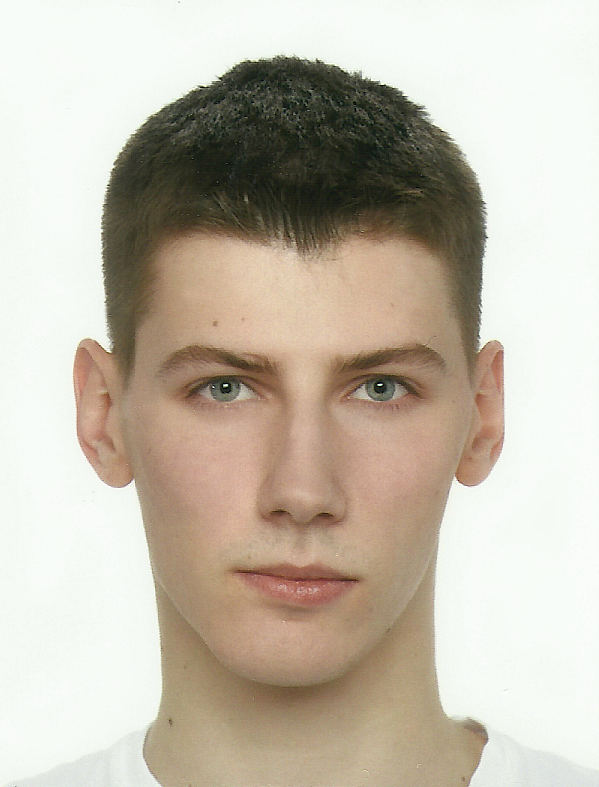
\includegraphics[width=4cm]{\ImgPath/zdjecie-kor.png}}

\opiekun{dr inż. Krzysztof Bieńkowski}
% opcjonalnie: \konsultant{prof. Dzielny Konsultant}
\terminwykonania{11 września 2017} % data złożenia - pokazana na stronie tytułowej
\datawydaniatematu{1 października 2016}
\rokakademicki{2016/2017}

% zakres pracy
\zakres{\begin{enumerate}
 \item Przegląd istniejących rozwiązań
 \item Projekty układu
 \item Budowa robota
 \item Implementacja programów sterujących
 \item Testy i analiza
\end{enumerate}}


% Podziekowanie - opcjonalne
\podziekowania{\noindent
{\Large Podziękowania}
\bigskip

Dziękuję bardzo serdecznie Rodzinie, Wykładowcom, Władzom Politechniki i Promotorowi - dr inż. Krzysztofowi Bieńkowskiemu

\bigskip

{\raggedleft
Mateusz Staszków

}

}

% To sa domyslne wartosci
% - mozna je zmienic, jesli praca jest pisana gdzie indziej niz w ZETiIS
% - mozna je wyrzucic jesli praca jest pisana w ZETiIS
\miasto{Warszawa}
\uczelnia{POLITECHNIKA WARSZAWSKA}
\wydzial{WYDZIAŁ ELEKTRYCZNY}
\instytut{INSTYTUT STEROWANIA \linebreak[1] I~ELEKTRONIKI PRZEMYSŁOWEJ}
\zaklad{ZAKŁAD MASZYN ELEKTRYCZNYCH}
\rodzajpracy{INŻYNIERSKA}
\kierunekstudiow{Automatyka i Robotyka}
%%% koniec od P.W

%\opinie{%
  %\newpage
\begin{center}
 {\large\bf  Opinia} \\
o pracy dyplomowej magisterskiej wykonanej przez dyplomanta\\
{\bf Zdolnego Studenta i Pracowitego Kolegę} \\
 Wydział Elektryczny, kierunek Informatyka,  Politechnika Warszawska\\
Temat pracy\\
\textit{\bf
TYTUŁ PRACY DYPLOMOWEJ
}\\
\end{center}
\medskip
\noindent
Kierownik pracy dyplomowej: {\bf dr inż. Adam Niewymagający}\\
Ocena pracy dyplomowej: {\bf bardzo dobry}

\medskip

\centerline{\bf Treść opinii}
   Celem pracy dyplomowej panów dolnego Studenta i Pracowitego Kolegi  było
opracowanie systemu pozwalającego symulować  i opartego o oprogramowanie o
otwartych źródłach (ang. Open Source). Jak piszą Dyplomanci, starali się opracować
system, który łatwo będzie dostosować do zmieniających się dynamicznie wymagań,
będzie miał niewielkie wymagania sprzętowe i umożliwiał dalszą łatwą rozbudowę oraz
dostosowanie go do potrzeb.
Przedstawiona do recenzji praca składa się z krótkiego wstępu jasno i
wyczerpująco opisującego oraz uzasadniającego cel pracy, trzech rozdziałów (2-4)
zawierających opis istniejących podobnych
rozwiązań, komponentów rozpatrywanychjako kandydaci do
tworzonego systemu i wreszcie zagadnień wydajności wirtualnych
rozwiązań. Piąty rozdział to opis przygotowanego przez
Dyplomantów środowiska obejmujący opis konfiguracji
środowiska oraz przykładowe ćwiczenia laboratoryjne. Ostatni
rozdział pracy to opis możliwości dalszego
rozwoju projektu. W ramach przygotowania pracy Dyplomanci zebrali i przedstawili w
bardzo przejrzysty sposób duży zasób informacji, co świadczy o dobrej orientacji
w nowoczesnej i ciągle intensywnie rozwijanej tematyce stanowiącej
zakres pracy i o umiejętności przejrzystego przedstawienia tych
wyników. Praca zawiera dwa dodatki, z których pierwszy obejmuje wyniki
eksperymentów i badań nad wydajnością, a drugi to źródła
skryptów budujących środowisko.

 Dyplomanci dość
dobrze zrealizowali postawione przed nimi zadanie,
wykazali się więc umiejętnością zastosowania w praktyce wiedzy
przedstawionej w rozdziałach 2-4.  Uważam, że cele postawione w założeniach pracy zostały pomyślnie
zrealizowane. Proponuję ocenę bardzo dobrą (5).

\vskip 1cm
{
\raggedleft
(data, podpis)\kern1cm

}
  %\newpage
  %\newpage
\begin{center}
 {\large\bf  Recenzja } \\
pracy dyplomowej magisterskiej wykonanej przez dyplomanta\\
{\bf Zdolnego Studenta i Pracowitego Kolegę} \\
 Wydział Elektryczny, kierunek Informatyka,  Politechnika Warszawska\\
Temat pracy\\
\textit{\bf
TYTUŁ PRACY DYPLOMOWEJ
}\\
\end{center}
\medskip
\noindent
Recenzent: {\bf prof. nzw. dr hab. inż. Jan Surowy}\\
Ocena pracy dyplomowej: {\bf bardzo dobry}
\medskip


\centerline{\bf Treść recenzji}
   Celem pracy dyplomowej panów dolnego Studenta i Pracowitego Kolegi  było
opracowanie systemu pozwalającego symulować  i opartego o oprogramowanie o
otwartych źródłach (ang. Open Source). Jak piszą Dyplomanci, starali się opracować
system, który łatwo będzie dostosować do zmieniających się dynamicznie wymagań,
będzie miał niewielkie wymagania sprzętowe i umożliwiał dalszą łatwą rozbudowę oraz
dostosowanie go do potrzeb.
Przedstawiona do recenzji praca składa się z krótkiego wstępu jasno i
wyczerpująco opisującego oraz uzasadniającego cel pracy, trzech rozdziałów (2-4)
zawierających bardzo solidny i przejrzysty opis: istniejących podobnych
rozwiązań (rozdz. 2), komponentów rozpatrywanychjako kandydaci do
tworzonego systemu (rozdz. 3) i wreszcie zagadnień wydajności wirtualnych
rozwiązań, zwłaszcza w kontekście współpracy  kilku elementów
 sieci (rozdział 4). Piąty rozdział to opis przygotowanego przez
Dyplomantów środowiska obejmujący opis konfiguracji
środowiska oraz przykładowe ćwiczenia laboratoryjne (5 ćwiczeń). Ostatni, szósty
rozdział pracy to krótkie zakończenie, które wylicza także możliwości dalszego
rozwoju projektu. W ramach przygotowania pracy Dyplomanci zebrali i przedstawili w
bardzo przejrzysty sposób duży zasób informacji o narzędziach, Rozdziały 2, 3 i 4 świadczą o dobrej orientacji
w nowoczesnej i ciągle intensywnie rozwijanej tematyce stanowiącej
zakres pracy i o umiejętności syntetycznego, przejrzystego przedstawienia tych
wyników. Drobne  mankamenty tej części pracy to zbyt skrótowe omawianie
niektórych zagadnień technicznych, zakładające dużą początkową wiedzę czytelnika
i dość niestaranne podejście do powołań na źródła.
Utrudnia to w pewnym stopniu czytanie pracy i zmniejsza jej wartość dydaktyczną
(a ta zdaje się być jednym z celów Autorów), ale jest zrekompensowane zawartością
merytoryczną. Praca zawiera dwa dodatki, z których pierwszy obejmuje wyniki
eksperymentów i badań nad wydajnością, a drugi to źródła
skryptów budujących środowisko. Praca
zawiera niestety dość dużą liczbę drobnych błędów redakcyjnych, ale nie wpływają
one w sposób istotny na na jej czytelność i wartość. W całej pracy przewijają
się samodzielne, zdecydowane wnioski Autorów, które są wynikiem własnych i
oryginalnych badań.  Rozdział 5 i dodatki pracy przekonują mnie, że Dyplomanci dość
dobrze zrealizowali postawione przed nimi zadanie. Pozwala to stwierdzić, że
wykazali się więc także umiejętnością zastosowania w praktyce wiedzy
przedstawionej w rozdziałach 2-4. Kończący pracę rozdział szósty świadczy o
dużym (ale moim zdaniem uzasadnionym) poczuciu własnej wartości i jest
świadectwem własnego, oryginalnego spojrzenia na tematykę przedstawioną w pracy
dyplomowej. Uważam, że cele postawione w założeniach pracy zostały pomyślnie
zrealizowane. Proponuję ocenę bardzo dobrą (5).

\vskip 1cm
{
\raggedleft
(data, podpis)\kern1cm

}
%}


\begin{document}
\maketitle

%-----------------
% Wstęp
%-----------------
\chapter{Wstęp}

  %-----------------
  % Zastosowanie robotów inspekcyjnych
  %-----------------
\section{Zastosowanie robotów inspekcyjnych}

Roboty inspekcyjne znajdują zastosowanie najczęściej w miejscach trudno dostępnych dla człowieka. O wiele mniej popularnym tematem jest wykorzystanie ich do inspekcji korytarzy budynków. Wykorzystanie robota w takim zakresie nie wymaga rozbudowanego systemu monitoringu i osób go nadzorujących w obserwowanym obiekcie. Przewagą poruszającej się maszyny jest przede wszystkim to, że może odwiedzić miejsca, które nie byłyby widoczne bez umieszczenia ogromnej ilości kamer w budynku. Zadaniem robotów inspekcyjnych jest odwiedzenie lub zeskanowanie każdego miejsca i upewnienie się czy wszystko jest zgodne z zaprogramowanym porządkiem. Obecnie jedną z głównych firm zajmujących się produkcją robotów inspekcyjnych jest General Electric \cite{ge}. 

Problem stabilizacji położenia w pionie dotyczy wielu gałęzi przemysłu, na przykład takich jak: produkcja jednoosobowych transportowych pojazdów typu Segway na lotniskach i w centrach handlowych \cite{segway}, układy balansujące na nierównych powierzchniach, czy nawet roboty humanoidalne \cite{humanoid}. 

Konstrukcja dwukołowego robota pozwala zmniejszyć wydatki energetyczne potrzebne na napędzanie robota. Umieszczając środek ciężkości jak najwyżej można sterować maszyną bardzo słabymi impulsami. Niestety w przypadku utraty równowagi konieczne jest zużycie dużej ilości energii, aby przywrócić pozycję pionową, dlatego program sterujący powinien być napisany jak najstaranniej. Dodatkowo taka konstrukcja sprawia, że robot jest bardzo zwinny i możliwe jest obracanie w miejscu (co jest przydatne do skanowania kolejnych sektorów obiektu).

Od strony matematycznej dwukołowy robot balansujący działa na zasadzie wahadła odwróconego. Jego zadaniem jest ciągłe utrzymywanie pionu z możliwie jak najmniejszymi odchyleniami. Jest to układ niestabilny i wymaga automatycznej regulacji - zadanie to spełnia kaskada regulatorów PID. W układzie za sprzężenia zwrotne odpowiadają czujniki położenia, a dokładniej przyspieszenia kątowego - akcelerometr, prędkości kątowej - żyroskop oraz prędkości liniowej - enkodery magnetyczne, które służą również do sterowania silnikami prądu stałego. Elektronika znajduje się na wytrawionych płytkach drukowanych. Obudowa została wykonana w technologii druku 3D z lekkiego tworzywa ABS. Układ jest zasilany z akumulatora litowo-polimerowego. Do komunikacji robota z otoczeniem służą czujniki ultradźwiękowe. Moduł Wi-Fi umożliwia bezprzewodową komunikację i odczyt wszystkich pomiarów. W celu wizualizacji odbieranych danych została napisana dedykowana aplikacja internetowa, jej kod został wgrany do modułu Wi-Fi, który pełni rolę serwera obsługującego protokół HTTP, dzięki czemu aplikacja może być obsługiwana przez jakiekolwiek urządzenie z przeglądarką internetową. Robot jest zaprojektowany tak, aby każdy element był jak najlżejszy i można było go łatwo wymienić. Stąd duża ilość śrub i mocowań na wcisk.

  %-----------------
  % Postawienie zadania
  %-----------------
\section{Postawienie zadania}

Zadaniem pracy jest opis konstrukcji autonomicznego i balansującego robota inspekcyjnego oraz przedstawienie działania za pośrednictwem analiz wykresów wygenerowanych w trakcie działania układu.

Budowa robota to złożone zadanie i wymaga podzielenia na mniejsze zagadnienia:
\begin{enumerate}
	\item Przeczytanie literatury na temat: 
    \begin{itemize}
    	\item balansujących i inspekcyjnych robotów komercyjnych, 
        \item dokumentacji technicznych mikrokontrolerów, czujników ultradźwiękowych, akcelerometrów i żyroskopów, modułów Wi-Fi, enkoderów, silników,
        \item dekodowania sygnałów z wyżej wymienionych czujników,
        \item szeregowej komunikacji przewodowej i bezprzewodowej,
        \item druku 3D,
        \item technologii wytwarzania płytek elektronicznych,
    \end{itemize}
	\item Zaprojektowanie:
    	\begin{itemize}
    		\item modelu matematycznego i modelu sterowania,
        	\item elektroniki w środowisku Autodesk EAGLE,
        	\item modelu 3D podzielonego na części w programie AutoCAD,
    	\end{itemize}
    \item Zakup elementów elektronicznych,
	\item Wydrukowanie części na drukarce 3D i sklejenie ich,
	\item Wytrawienie płytek drukowanych,
	\item Przylutowanie elementów elektronicznych do płytek,
	\item Skonfigurowanie środowisk programistycznych,
    \item Wzajemne skomunikowanie mikrokontrolerów,
    \item Oprogramowanie czujników,
    \item Implementacja:
    	\begin{itemize}
    		\item sterownika silników prądu stałego,
        	\item bezprzewodowej komunikacji mikrokontrolera przez sieć Wi-Fi,
        	\item układu sterowania położenia w pionie,
            \item systemu autonomicznego poruszania się robota,
            \item systemu zbierania danych o otoczeniu (skanowania),
            \item aplikacji internetowej wizualizującej zebrane pomiary,
    	\end{itemize}
    \item Testy i analiza,
    \item Wnioski.
\end{enumerate}

%-----------------
% Mechanika
%-----------------
\chapter{Mechanika}
Robot został zaprojektowany tak, aby był jak najlżejszy. Ułatwia to sterowanie jego położeniem przy odpowiednio dobranych silnikach. Środek ciężkości znajduje się jak najwyżej, co przekłada się na ułatwienie sterowania położenia w pionie - układ gwałtowniej odpowiada na zadane wartości.

  %-----------------
  % Parametry ogólne
  %-----------------
\section{Parametry ogólne}

\noindent Masa: ok. 978 g\\
Wymiary: 95 mm x 180 mm x 306 mm\\
Wysokość środka masy: 162,6 mm\\
Moment bezwładności dla osi położonej w środku masy: 0,01 kgm$^2$\\

\begin{figure}[!htbp]
	\begin{center}
\centering
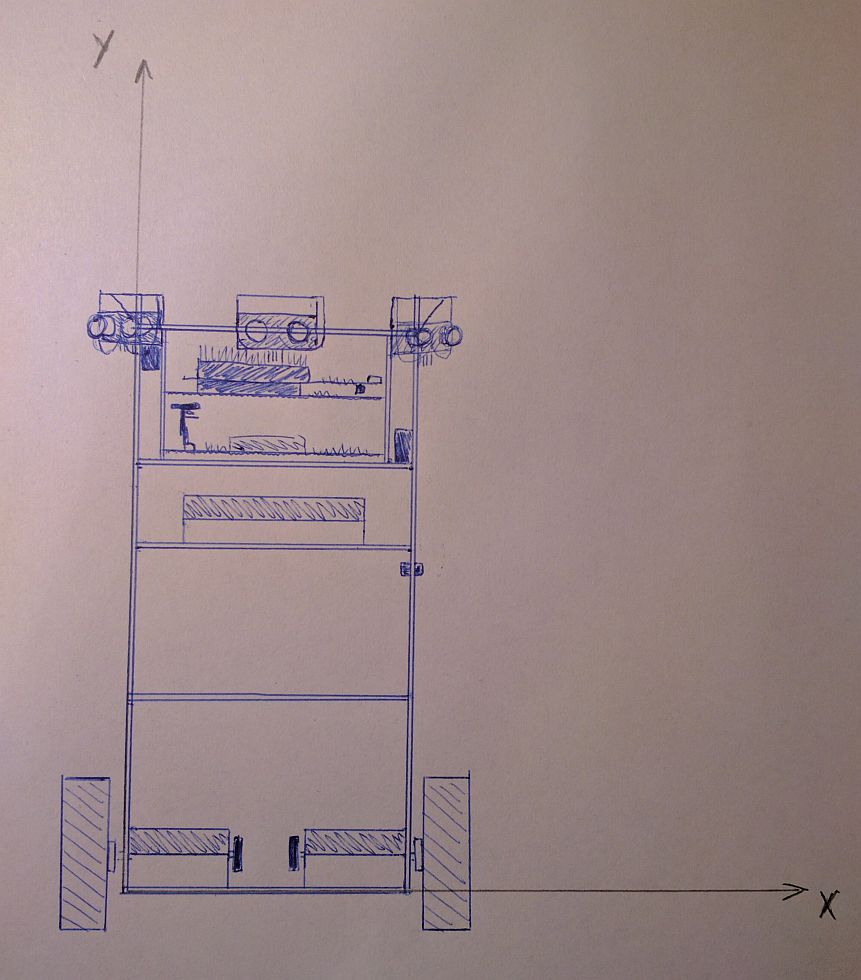
\includegraphics[scale=0.25]{\ImgPath/koncepcja.jpg}
\end{center}
	\caption{Koncepcja obudowy robota [opracowanie własne]}
	\label{model3d}
\end{figure}

\newpage
  %-----------------
  % Model 3D
  %-----------------
\section{Model 3D}
Model został zbudowany w programie Autodesk AutoCAD 2017. Następnie został podzielony na części w taki sposób, aby wydruk przestrzenny był jak najmniej kłopotliwy. Każda część ma wymiary nie większe niż 100 mm x 180 mm x 80 mm. Następnie modele zostały wyeksportowane do formatu STL, który jest obsługiwany przez większość drukarek 3D.

\begin{figure}[!htbp]
	\begin{center}
\centering
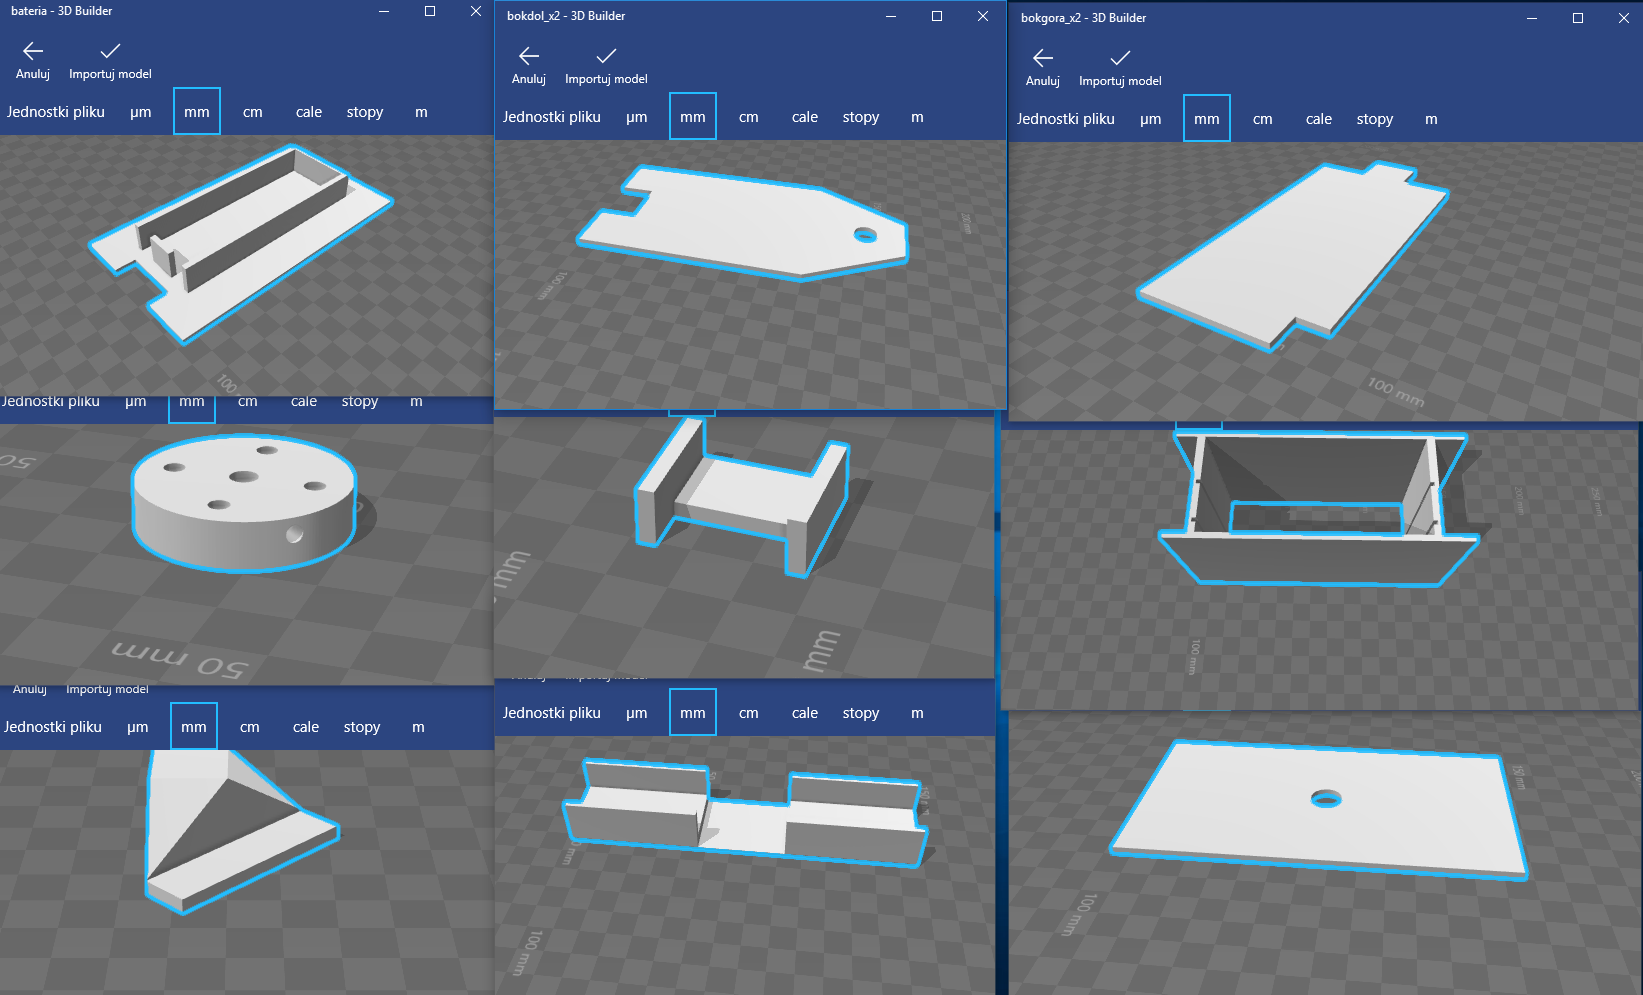
\includegraphics[scale=0.3]{\ImgPath/druki3d.PNG}
\end{center}
	\caption{Model 3D podzielony na części i wyeksportowany do STL [opracowanie własne]}
	\label{druki3d}
\end{figure}

\subsection{Obudowa}

\noindent Zmierzone dane:
\begin{itemize}
\item masa: 402 g,
\item wymiary: 95 mm x 180 mm x 306 mm.
\end{itemize}

Elementy obudowy zostały w całości wydrukowane na drukarce 3D, a następnie połączone acetonem. Proces adhezyjnego klejenia części jest możliwy poprzez użycie jako materiału do drukowania tworzywa ABS - kopolimeru akrylonitrylo-butadieno-styrenowego, który reagując z acetonem rozpuszcza się, umożliwiając, poprzez zbliżenie do niego innego materiału na przyklejenie się. 
\newpage
\noindent Obudowa składa się z czterech segmentów - kolejno od dołu:
\begin{itemize}
\item segment silników - odpowiadający za napęd robota, silniki są przykręcone do ścian bocznych za pomocą śrub i zaciśnięte plastikowymi opaskami zaciskowymi do dolnej półki, a także znajdują się w specjalnie zaprojektowanych wyżłobieniach, aby ograniczyć ich ruch. W ścianach bocznych umieszczono łożyska, w których znajdują się wały silników,
\item część akumulatora - odpowiadająca za zasilanie, akumulator ma swój koszyk, co umożliwia łatwą wymianę i odpowiednie usztywnienie pakietu ogniw,
\item część elektroniczna: ściany z otworami na wciśnięcie płytek laminowanych,
\item część komunikacyjna: znajdują się tu miejsca na 3 czujniki ultradźwiękowe wraz z konwerterem logicznych poziomów napięć (w osobnym układzie scalonym), moduł Wi-Fi oraz koszyk na żyroskop/akcelerometr.
\end{itemize}

\begin{figure}[!htbp]
	\begin{center}
\centering
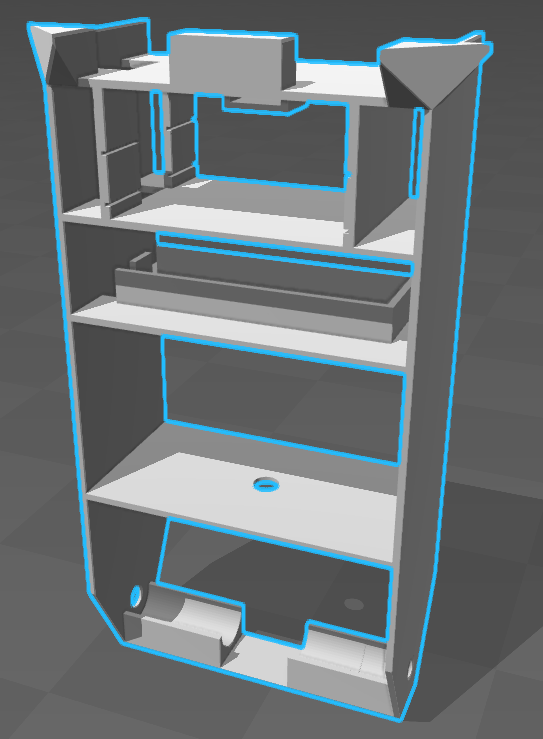
\includegraphics[scale=0.4]{\ImgPath/model3d.PNG}
\end{center}
	\caption{Cała obudowa zaprojektowana w programie Autodesk AutoCAD i wyeksportowana do pliku STL [opracowanie własne]}
	\label{model3d}
\end{figure}

\newpage

  %-----------------
  % Napęd
  %-----------------
\section{Napęd}

Do napędu robota zostały użyte silniki prądu stałego firmy Pololu na napięcie 12 V z przekładnią 9,68 : 1 (25Dx48L) i enkoderem CPR 48, których wały opierają się na łożyskach kulkowych umieszczonych w ścianach bocznych.\\
\\
Parametry silnika \cite{pololu}:
\begin{itemize}
\item masa: 0,095 kg,
\item wymiary: średnica 25 mm, długość korpusu 78,7 mm,
\item moment obrotowy: 0,15 Nm,
\item prędkość obrotowa:	770 obr/min,
\item średni pobór prądu:	200 mA,
\item maksymalny pobór prądu:	2100 mA,
\item rozdzielczość enkodera: 48 impulsów na obrót (po przekładni 464).
\end{itemize}

\begin{figure}[!htbp]
	\begin{center}
\centering
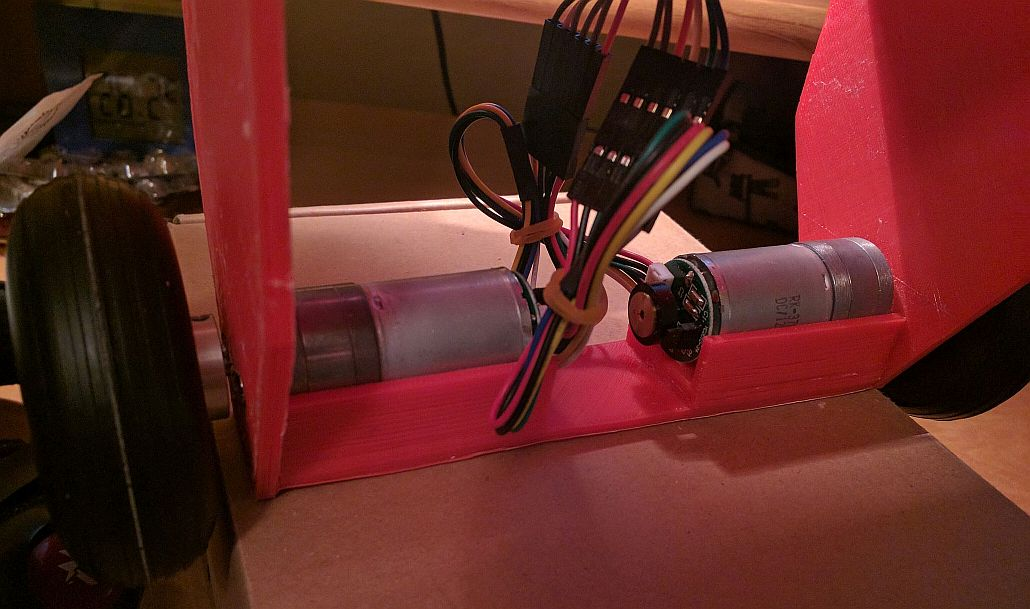
\includegraphics[scale=0.4]{\ImgPath/silnikidc.jpg}
\end{center}
	\caption{Silnik DC Pololu 12 V [opracowanie własne]}
	\label{schematKomunikacji}
\end{figure}

\newpage
\noindent Do wału silnika zostały dopasowane łożyska kulkowe o średnicach 4 mm (wewnętrzna) i 12 mm (zewnętrzna) oraz grubości 4 mm. Dzięki nim następuje lżejsze przełożenie napędu na koła z minimalnym tarciem. Obniżają nacisk na wał silnika.

\begin{figure}[!htbp]
	\begin{center}
\centering
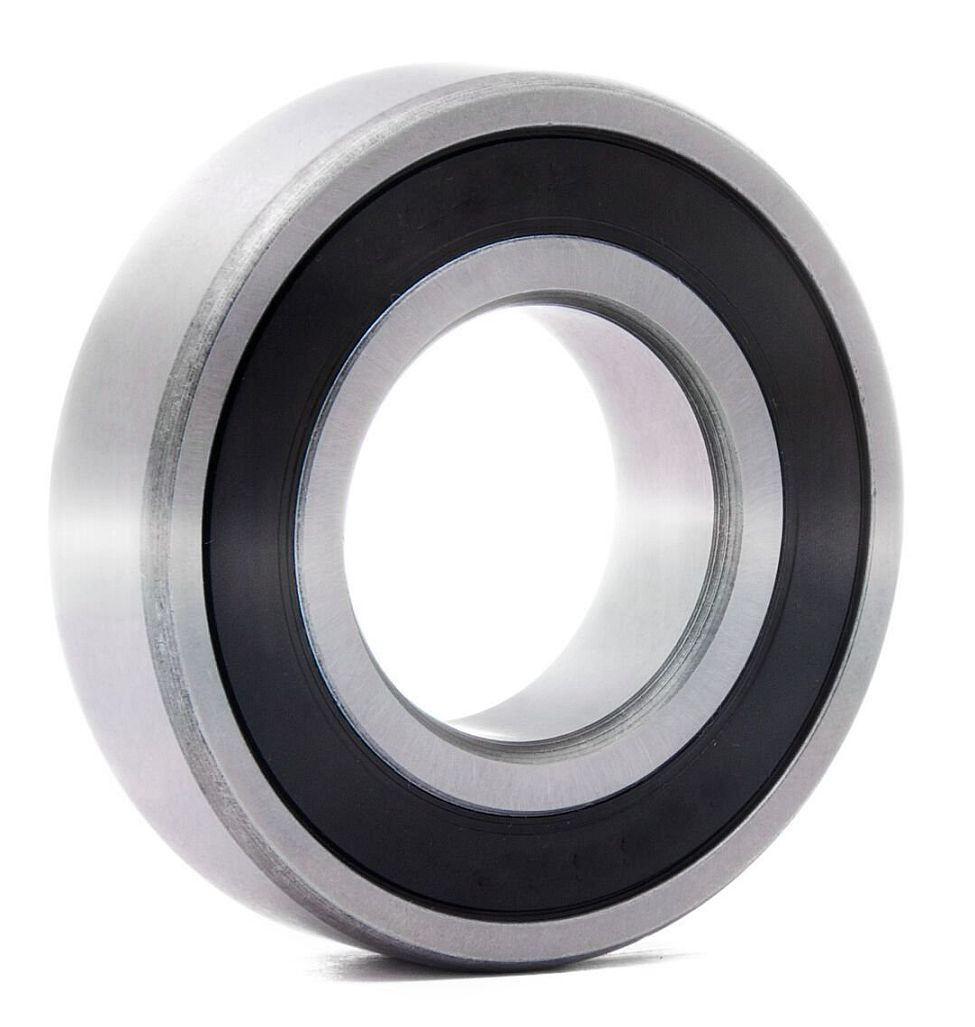
\includegraphics[scale=0.1]{\ImgPath/lozysko.jpg}
\end{center}
	\caption{Łożysko kulkowe \cite{lozysko}}
	\label{schematKomunikacji}
\end{figure}
 
  %-----------------
  % Koła
  %-----------------
\section{Koła}

W konstrukcji zostały użyte lekkie poliuretanowe koła z plastikową piastą, charakteryzujące się niską ceną i dostateczną przyczepnością.\\
Parametry koła:
\begin{itemize}
\item średnica opony: 70 mm,
\item szerokość opony: 24 mm,
\item średnica otworu: 4 mm,
\item średnica plastikowej piasty: 35 mm,
\item waga: 30 g.
\end{itemize}

Do połączenia kół z krótkim wałem silnika zostały skonstruowane specjalne łączniki na śruby. Ich działanie polega na odpowiednio mocnym zaciśnięciu bocznej śruby o średnicy 2,5 mm. Wymagane jest w tym momencie specjalne ułożenie, w środku łącznika, wału silnika, którego przekrój nie jest idealnym okręgiem, lecz zawiera delikatne zeszlifowanie (kształtem przypomina literę D). Po dociśnięciu śruby w miejsce tego szlifu jakikolwiek luz zostanie wyeliminowany.

\begin{figure}[!htbp]
	\begin{center}
\centering
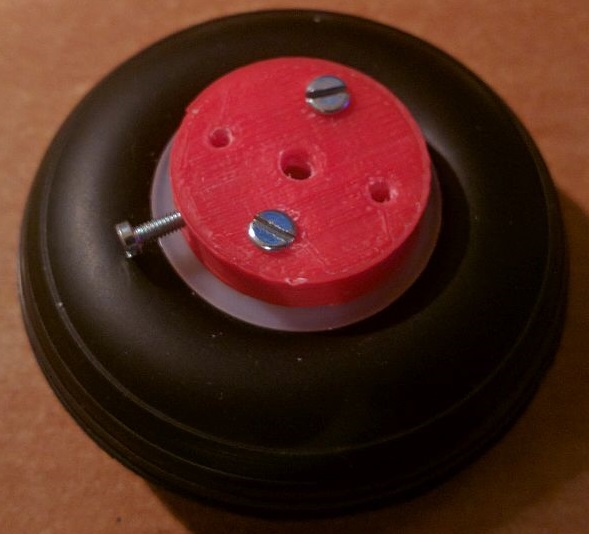
\includegraphics[scale=0.3]{\ImgPath/hub.jpg}
\end{center}
	\caption{Hub mocujący wał silnika z kołem [opracowanie własne]}
	\label{schematKomunikacji}
\end{figure}

Po testach wytrzymałościowych okazało się, że plastikowe tworzywo ABS nie wytrzymało dużych naprężeń śruby na wał silnika i uległo odkształceniu, dlatego zostały zastosowane uniwersalne aluminiowe huby mocujące z otworem na 4 mm.

\begin{figure}[!htbp]
	\begin{center}
\centering
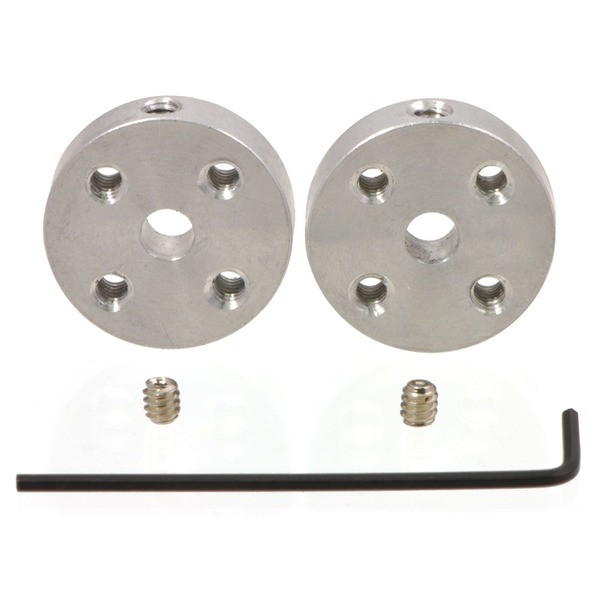
\includegraphics[scale=0.35]{\ImgPath/huby.jpg}
\end{center}
	\caption{Aluminiowe huby mocujące \cite{huby}}
	\label{schematKomunikacji}
\end{figure}

  %-----------------
  % Matematyczny model układu
  %-----------------
\section{Matematyczny model układu}

Robot jest zbudowany w przybliżeniu symetrycznie w odniesieniu do szerokości i długości, więc po zastosowaniu uproszczenia, środek masy wymaga przeprowadzenia dokładnych obliczeń jedynie w odniesieniu do wysokości. Reszta wartości będzie się pokrywała ze środkiem geometrycznym bryły. Przy obliczeniach położenie i masa przewodów zostały ujęte w dużym przybliżeniu.\\

Środek masy i moment bezwładności zostały obliczone poprzez podzielenie robota na obiekty i wyliczenie dla każdego środka masy i momentu bezwładności, a następnie zsumowanie wszystkich składowych w programie Microsoft Excel 2013.

\begin{figure}[!htbp]
	\begin{center}
\centering
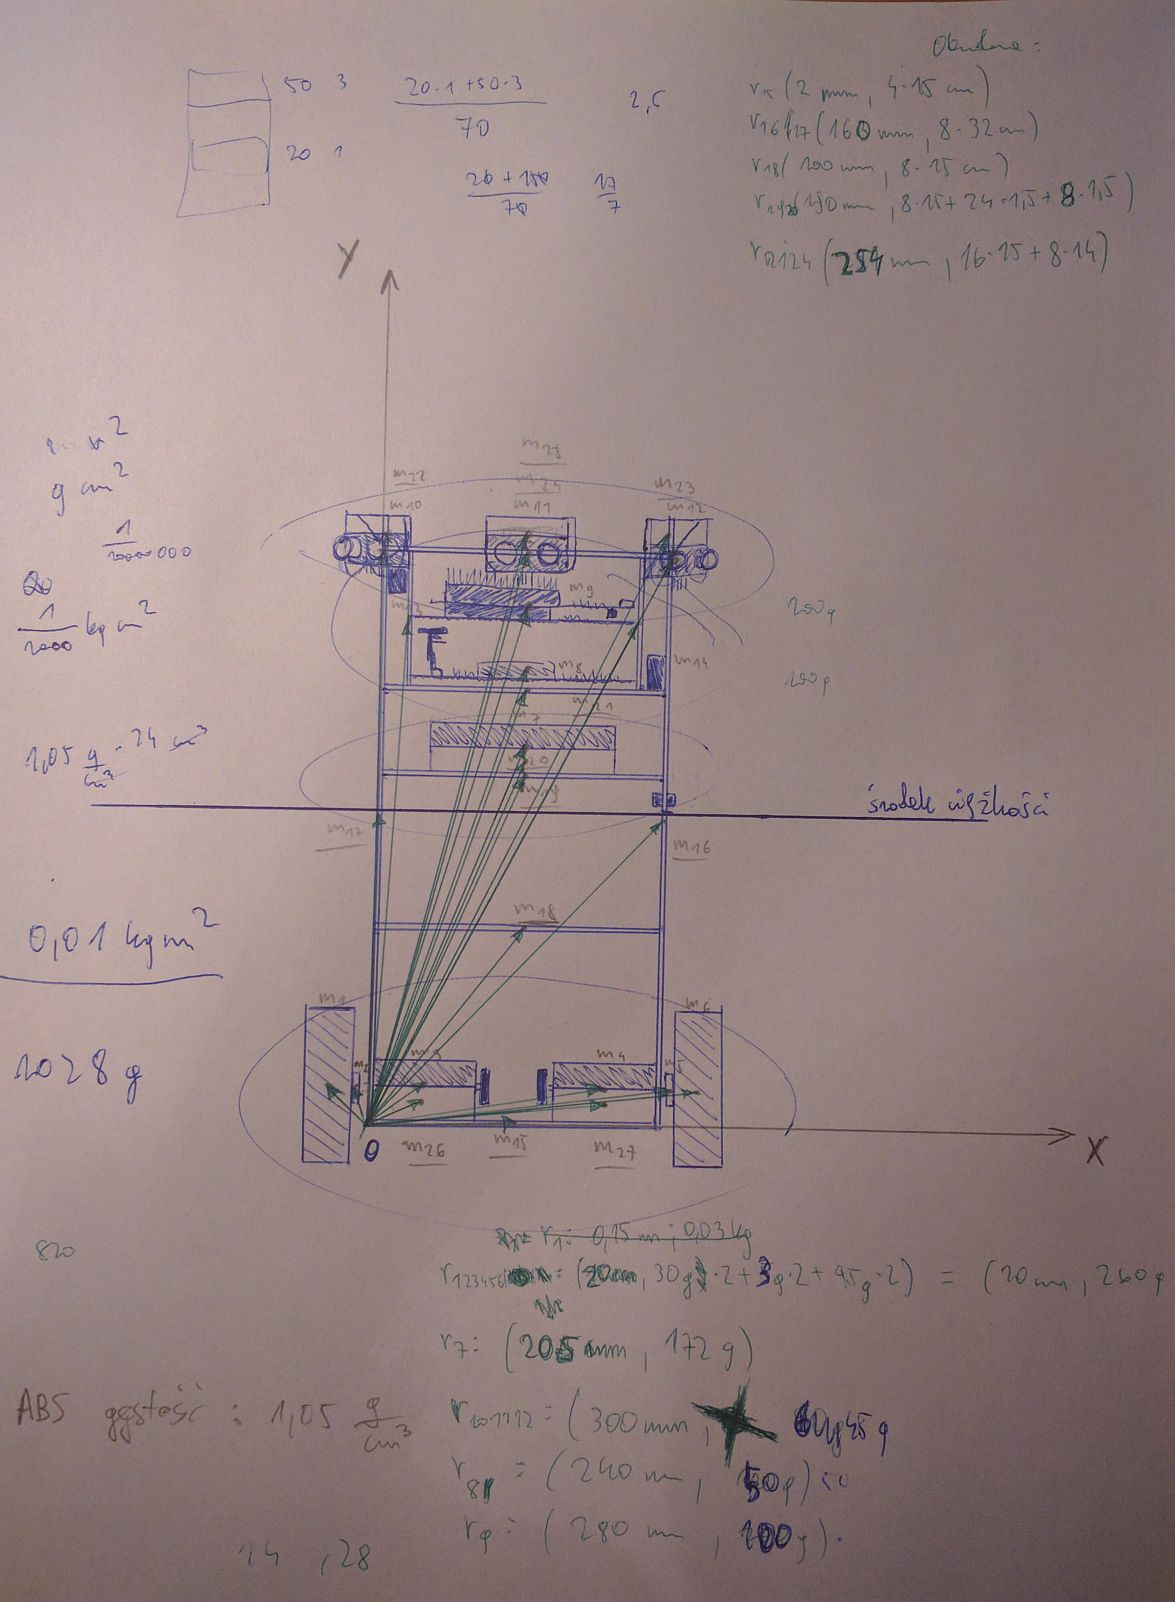
\includegraphics[scale=0.3]{\ImgPath/wektory.jpg}
\end{center}
	\caption{Wektory środków geometrycznych poszczególnych obiektów [opracowanie własne]}
	\label{schematKomunikacji}
\end{figure}
\newpage
\noindent Obliczone dane bryły:
\begin{itemize}
\item wysokość środka masy obudowy: 162,6 mm,
\item moment bezwładności obudowy: 0,01 kgm$^2$.
\end{itemize}

\noindent Obliczenia zostały wykonane w programie Microsoft Excel 2013:

\begin{figure}[!htbp]
	\begin{center}
\centering
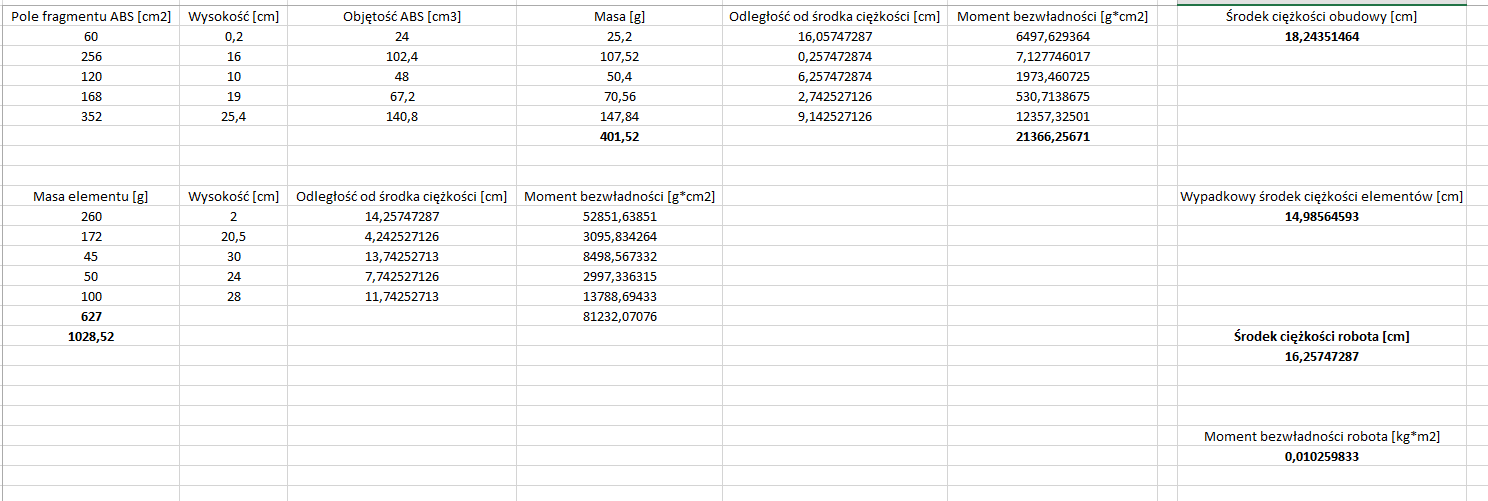
\includegraphics[scale=0.37]{\ImgPath/i.PNG}
\end{center}
	\caption{Obliczenie środka ciężkości i momentu bezwładności robota w programie Microsoft Excel 2013 [opracowanie własne]}
	\label{schematKomunikacji}
\end{figure}

\newpage
  %-----------------
  % Wyznaczenie równań liniowych układu
  %-----------------
\section{Wyznaczenie równań liniowych układu}


Dwukołowego robota balansującego można przedstawić jako układ odwróconego wahadła, który przypomina patyk znajdujący się na wózku, na który działa siła z zewnątrz. Układ taki wygląda następująco:\\

\begin{figure}[!htbp]
	\begin{center}
\centering
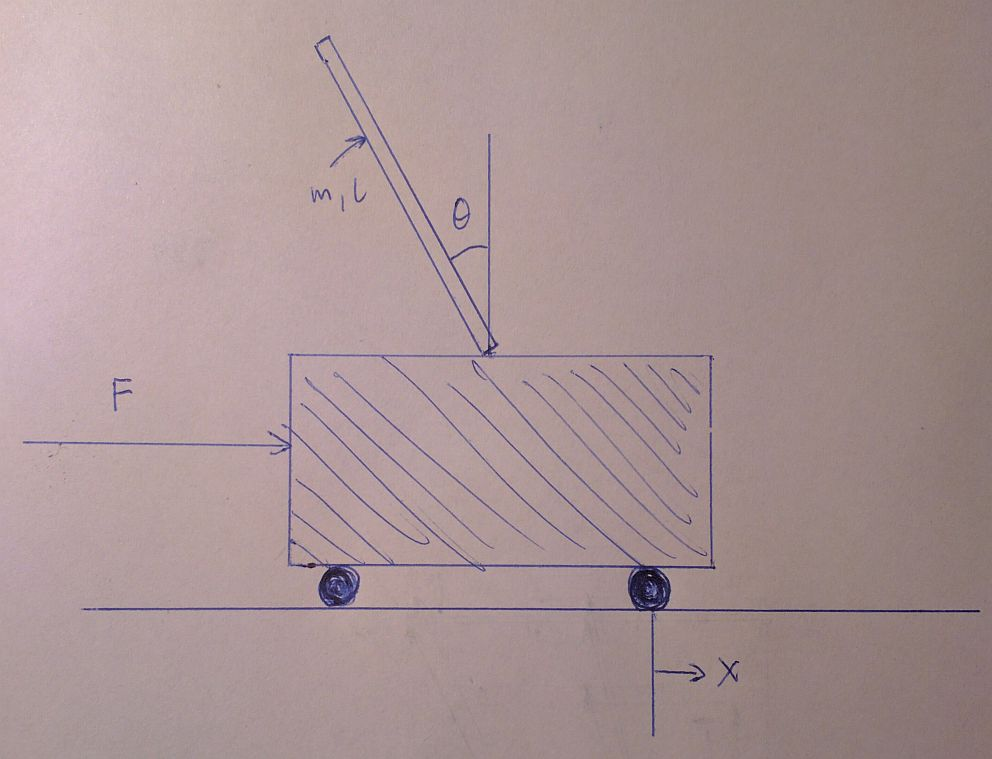
\includegraphics[scale=0.2]{\ImgPath/wahadlo.jpg}
\end{center}
	\caption{Układ wahadła odwróconego [opracowanie własne]}
	\label{schematKomunikacji}
\end{figure}

\noindent Równania opisujące model:\\
\\
Wzór 2.1: $F=(M+m)\ddot{x}+b\dot{x}+ml\ddot{\theta}$cos$\theta-ml\dot{\theta}^2$sin$\theta$ \\
Wzór 2.2: $-ml\ddot{x}$cos$\theta=(I+ml^2)\ddot{\theta}+mgl$sin$\theta$ \\
\\
Dane układu:
\begin{itemize}
\item M - masa wózka: 0 kg (wózek słuzył tylko do zilustrowania sytuacji),
\item m - masa odwróconego wahadła: 1 kg,
\item I - moment bezwładności odwróconego wahadła: 0.01 kgm$^2$,
\item F - siła działająca na wózek,
\item x - położenie wózka - zmienna stanu mierzona w metrach,
\item $\theta$ - wychylenie wahadła od pionu - zmienna stanu mierzona w stopniach,
\item b - współczynnik tarcia wózka o podłoże: ok. 0.1 Ns/m, 
\item l - odległość od środka masy: 0.137 m,
\item g - przyspieszenie ziemskie w Warszawie: 9.8123 m/s$^2$.
\end{itemize} 

\noindent W przypadku robota balansującego na dwóch kołach równanie upraszacza się do postaci:\\
\\
Wzór 2.3: $F=m\ddot{x}+b\dot{x}+ml\ddot{\theta}$cos$\theta-ml\dot{\theta}^2$sin$\theta$ \\
Wzór 2.4: $-ml\ddot{x}$cos$\theta=(I+ml^2)\ddot{\theta}+mgl$sin$\theta$ \\
\\
Powyższe równania są nieliniowe, więc po linearyzacji w otoczeniu punktu $\theta=\pi$ otrzymano następujące równania ($\theta=\pi+\phi$, gdzie $\phi$ reprezentuje małe odchylenia wahadła, a u to wejście układu):\\
\\
Wzór 2.5: $u=m\ddot{x}+b\dot{x}-ml\ddot{\phi}$ \\
Wzór 2.6: $ml\ddot{x}=(I+ml^2)\ddot{\phi}-mgl\phi$ \\

\noindent Opis układu w przestrzeni zmiennych stanu:\\
\\
\noindent Wzór 2.7: $\dot{x}=Ax+Bu$ \\
Wzór 2.8: $y=Cx+Du$ \\
\\
\\Wzór 2.9: $
     \begin{bmatrix}
       \dot{x} \\
       \ddot{x} \\
       \dot{\phi} \\
       \ddot{\phi}
     \end{bmatrix}
     =
     \begin{bmatrix}
       0 & 1 & 0 & 0          \\
       0 & \frac{-(I+ml^2)b}{Im} & \frac{mgl^2}{I} & 0 \\
       0 & 0 & 0 & 1 \\
       0 & \frac{-lb}{I} & \frac{mgl}{I} & 0 
     \end{bmatrix}
     \begin{bmatrix}
       x \\
       \dot{x} \\
       \phi \\
       \dot{\phi}
     \end{bmatrix}
     +
     \begin{bmatrix}
       0 \\
       \frac{I+ml^2}{Im} \\
       0 \\
       \frac{l}{I}
     \end{bmatrix}
     u\\$
Wzór 2.10: 
$y=
     \begin{bmatrix}
       1 & 0 & 0 & 0 \\
       0 & 0 & 1 & 0 
     \end{bmatrix}
     \begin{bmatrix}
       x \\
       \dot{x} \\
       \phi \\
       \dot{\phi}
     \end{bmatrix}
     +
     \begin{bmatrix}
       0 \\
       0 
     \end{bmatrix}
     u
$
\\
\\

\noindent Po wstawieniu liczb:\\
\\Wzór 2.11:$
     \begin{bmatrix}
       \dot{x} \\
       \ddot{x} \\
       \dot{\phi} \\
       \ddot{\phi}
     \end{bmatrix}
     =
     \begin{bmatrix}
       0 & 1 & 0 & 0          \\
       0 & -0,2877 & 18,4167 & 0 \\
       0 & 0 & 0 & 1 \\
       0 & -1,37 & 134,4285 & 0 
     \end{bmatrix}
     \begin{bmatrix}
       x \\
       \dot{x} \\
       \phi \\
       \dot{\phi}
     \end{bmatrix}
     +
     \begin{bmatrix}
       0 \\
       2,8769 \\
       0 \\
       13,7
     \end{bmatrix}
     u\\$
Wzór 2.12:
$y=
     \begin{bmatrix}
       1 & 0 & 0 & 0 \\
       0 & 0 & 1 & 0 
     \end{bmatrix}
     \begin{bmatrix}
       x \\
       \dot{x} \\
       \phi \\
       \dot{\phi}
     \end{bmatrix}
     +
     \begin{bmatrix}
       0 \\
       0 
     \end{bmatrix}
     u
$


\chapter{Elektronika}

  %-----------------
  % Zasilanie
  %-----------------

\section{Zabezpieczenie elektroniki}

Elektronika może ulec uszkodzeniu ze względu na wiele czynników: silne pole magnetyczne, wysoka temperatura, za duży prąd lub napięcie. W układzie zostało zastosowanych kilka zabezpieczeń:
\begin{itemize}
\item akumulator jest podłączony do przełącznika na prąd do 15 A, który służy jako główny włącznik robota,
\item dodatni sygnał z akumulatora przechodzi przez szeregowo wpięty rezystor 0,1~$\Omega$ 5 W, który ogranicza przepływ prądu do 7 A, ze względu na swoją wytrzymałość. Może również służyć do pomiaru prądu pobieranego z akumulatora,
\item do dwukanałowego mostka w sterowniku silników, został dołączony radiator w formie dwóch lekkich blaszek aluminiowych (fragmentów ościeżnicy)
\item przy każdym układzie scalonym zostały dołączone kondensatory i rezystory zgodnie z notami katalogowymi, aby urządzenia nie uległy uszkodzeniu i działały poprawnie.
\end{itemize}

  %-----------------
  % Układ zasilający
  %-----------------
\section{Układ zasilający}

Jedną z dwóch wytrawionych płytek drukowanych jest ta przeznaczona do wyższych napięć i prądów niż te występujące w części logicznej. Dominującym napięciem w tej części jest 12 V o natężeniu do 5 A, dlatego ścieżki są odpowiednio szersze, aby zapewnić mniejsze spadki napięcia.

\subsection{Akumulator}

Do zasilania został użyty pakiet ogniw litowo-polimerowych firmy Redox. Akumulator został wybrany ze względu na to, że dostarcza dużo energii przy małych rozmiarach, a także może być stale obciążony dużym prądem. \\
\\
\noindent Dane techniczne \cite{aku}:
\begin{itemize}
\item napięcie nominalne: 11,1 V (pełne naładowanie: 12,6 V),
\item pojemność: 2200 mAh,
\item prąd rozładowania: 30 C (66 A),
\item wymiary: 115 mm x 34 mm x 20 mm,
\item masa: 172 g.
\end{itemize}

W najbardziej pesymistycznym przypadku robot może pobierać do 5 A ciągłego prądu. Przy pojemności 2200 mAh daje to minimalny czas pracy około 26 minut. Natomiast w przypadku zwykłej jazdy, bez większych zakłóceń z zewnątrz, robot może pobrać ok. 1 A, co przekłada się na pięciokrotnie dłuższe działanie. W 130 minut powinno dać się zmapować kilka razy w ciągu nocy całe piętro budynku.

\begin{figure}[!htbp]
	\begin{center}
\centering
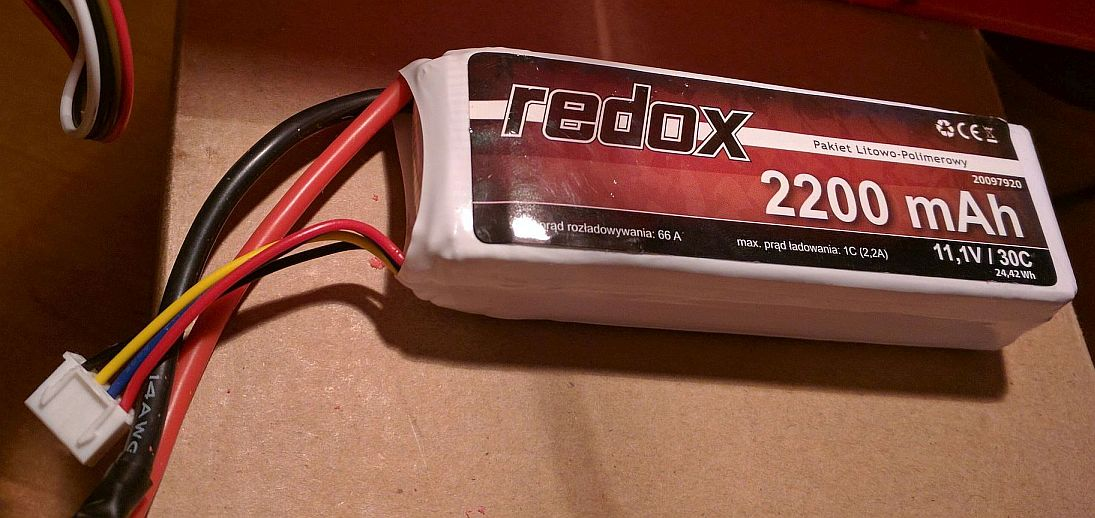
\includegraphics[scale=0.4]{\ImgPath/lipo.jpg}
\end{center}
	\caption{Akumulator litowo-polimerowy firmy Redox [opracowanie własne]}
	\label{schematKomunikacji}
\end{figure}

\newpage

\begin{figure}[!htbp]
	\begin{center}
\centering
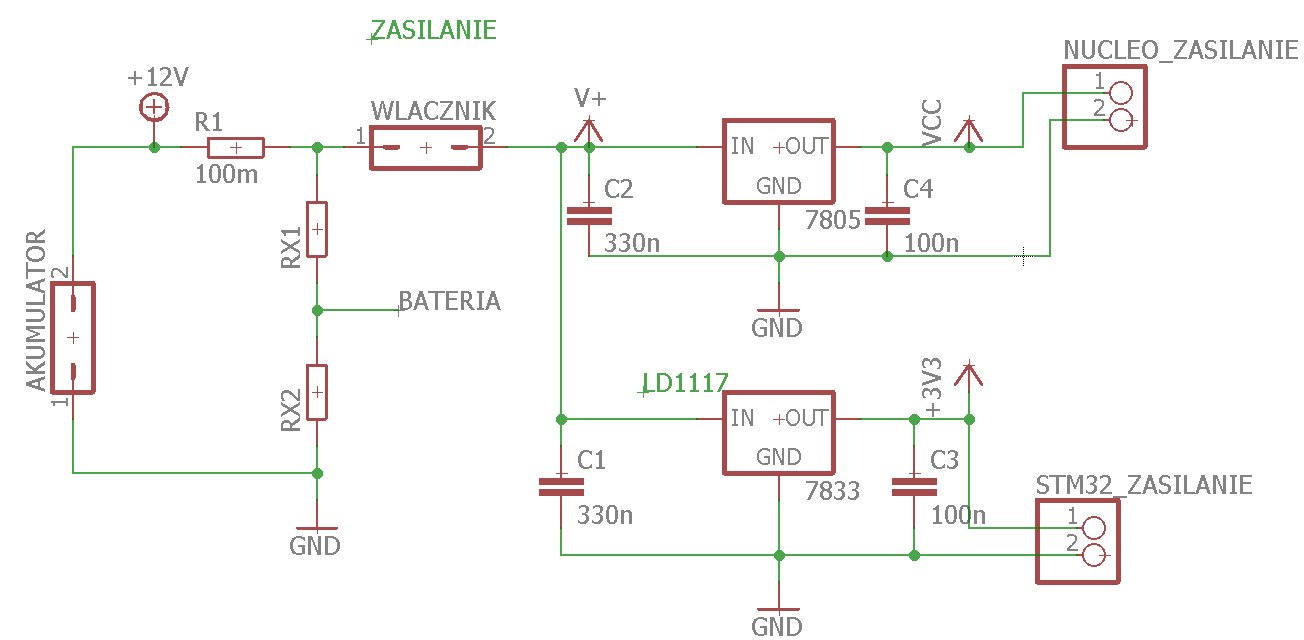
\includegraphics[scale=0.4]{\ImgPath/zasilanie_sch.PNG}
\end{center}
	\caption{Schemat całego układu zasilającego w programie EAGLE [opracowanie własne]}
	\label{schematKomunikacji}
\end{figure}

Na wyjściu z akumulatora znajduje się dzielnik napięcia, który pozwala na pomiar napięcia przez przetwornik analogowo-cyfrowy mikrokontrolera STM32F103RBT6. Napięcie ze źródła zasilania jest bezpośrednio przekazywane tylko do silników (na dwukanałowy mostek), a na układy logiczne dostarczane jest poprzez stabilizatory liniowe 7805 na 5 V i LD1117VC33 na 3,3 V. Stabilizatory są w obudowach TO-220, co ułatwia ich chłodzenie. Zasilają części logiczne, więc wbudowana blaszka odprowadzająca ciepło wystarczy, żeby cały układ się nie przegrzał. Do stabilizatorów zostały dołączone kondensatory MKT 330 nF i ceramiczne 100 nF zgodnie z notami katalogowymi \cite{7805,LD1117}.

\begin{figure}[!htbp]
	\begin{center}
\centering
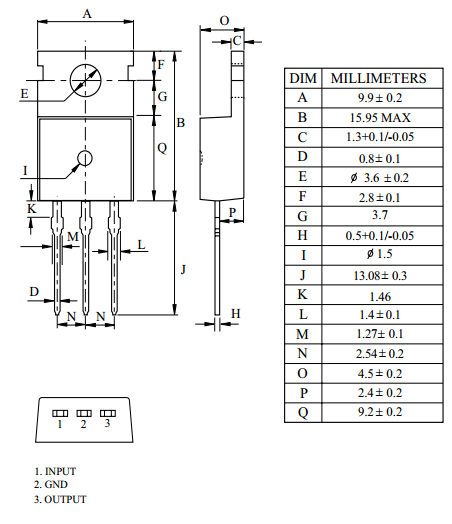
\includegraphics[scale=0.4]{\ImgPath/7805.PNG}
\end{center}
	\caption{Układ 7805 [źródło: \cite{7805}, strona 1]}
	\label{schematKomunikacji}
\end{figure}
\newpage
\begin{figure}[!htbp]
	\begin{center}
\centering
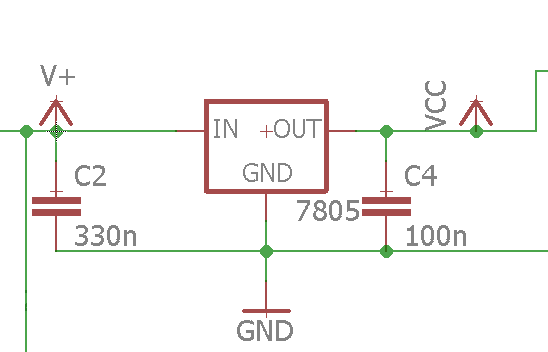
\includegraphics[scale=0.4]{\ImgPath/7805e.PNG}
\end{center}
	\caption{Schemat połączeń układu 7805, program EAGLE [opracowanie własne]}
	\label{schematKomunikacji}
\end{figure}

\begin{figure}[!htbp]
	\begin{center}
\centering
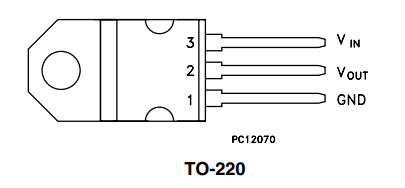
\includegraphics[scale=0.6]{\ImgPath/ld1117.PNG}
\end{center}
	\caption{Układ LD1117VC33 [źródło: \cite{LD1117}, strona 3]}
	\label{schematKomunikacji}
\end{figure}

\begin{figure}[!htbp]
	\begin{center}
\centering
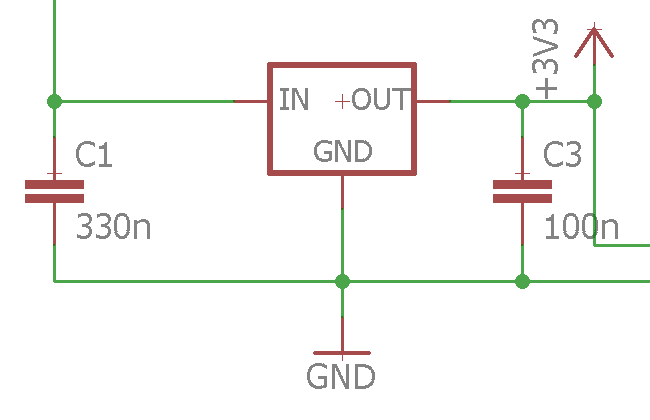
\includegraphics[scale=0.4]{\ImgPath/ld1117e.PNG}
\end{center}
	\caption{Schemat połączeń układu LD1117VC33, program EAGLE [opracowanie własne]}
	\label{schematKomunikacji}
\end{figure}

\newpage

Napięcie 5 V jest kierowane do czujników ultradźwiękowych HC-SR04, napięcie 3,3 V służy do zasilenia modułu Wi-Fi ESP8266. Natomiast obydwa poziomy napięć są kierowane do zasilania płytki NUCLEO F103RB i konwertera napięć logicznych SparkFun.

\subsection{Ładowarka}

Ładowanie pakietów ogniw litowo-polimerowych wymaga stosowania ładowarek mikroprocesorowych z odpowiednim algorytmem ładowania, wyposażonych w układy balancerów, które równomiernie ładują każde ogniwo. W celu uniknięcia trwałych uszkodzeń ogniwa, powinno się nie rozładowywać go poniżej 3V, czyli w przypadku całego pakietu napięcie nie powinno osiągnąć wartości poniżej 9 V (przy założeniu, że wszystkie ogniwa mają w danej chwili taką samą wartość napięcia).

W celu zachowania powyższych zasad została zastosowana ładowarka sieciowa firmy Redox. Specyfikacja \cite{ladowarka}:
\begin{itemize}
\item Napięcie wejściowe: 100 - 240 V AC 50 / 60 Hz,
\item Prąd ładowania: do 1000 mA,
\item Obsługiwane pakiety: 2-3 ogniwowe litowo-polimerowe (7,4  V i 11,1 V),
\item Wbudowany balancer ogniw,
\item Długość przewodów: 150 cm,
\item Wymiary: 96 mm x 55 mm x 33 mm.
\end{itemize}

\begin{figure}[!htbp]
	\begin{center}
\centering
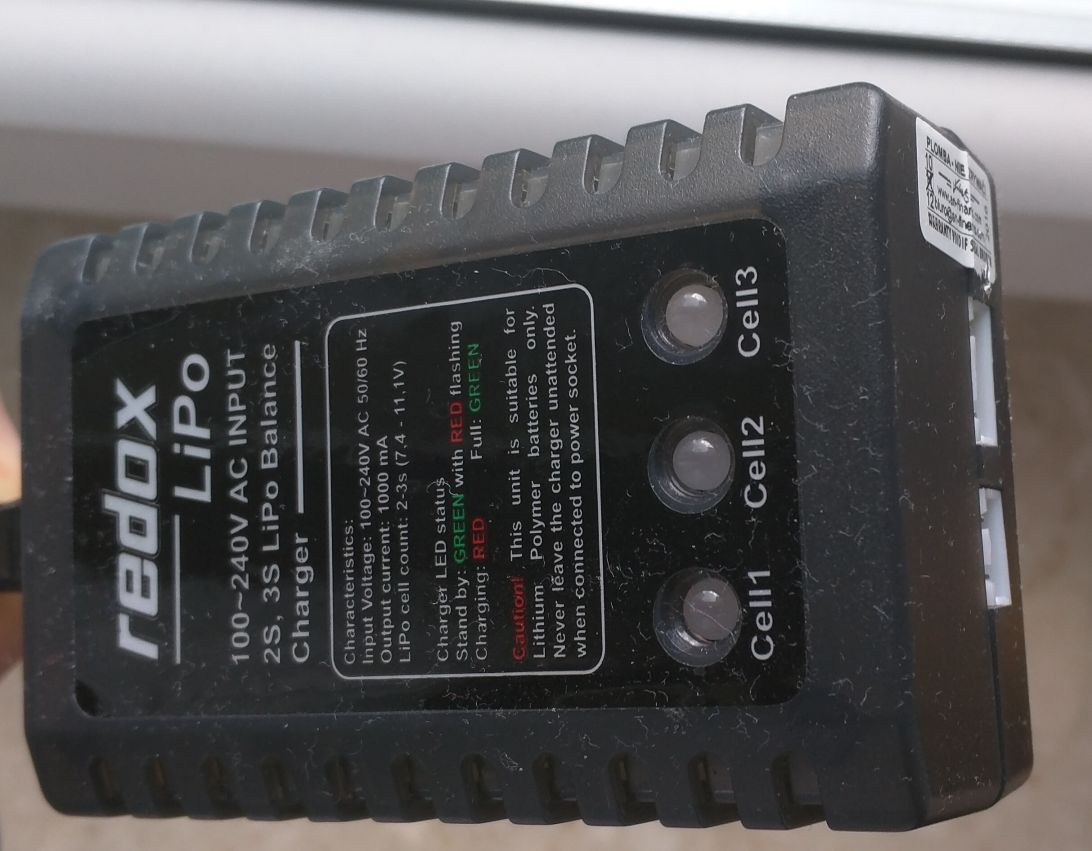
\includegraphics[scale=0.22]{\ImgPath/ladowarka.jpg}
\end{center}
	\caption{Ładowarka sieciowa Redox [opracowanie własne]}
	\label{schematKomunikacji}
\end{figure}

\subsection{Enkodery magnetyczne CPR 48}

Zastosowane enkodery są zintegrowane z używanymi silnikami. Ich działanie jest oparte na zjawisku Halla - sensory wykrywają impulsy na obracającej się tarczy magnetycznej umieszczonej z tyłu silnika. Używane enkodery kwadraturowe posiadają rozdzielczość 48 impulsów na obrót, co po przemnożeniu przez wartość przekładni 9,7:1 - daje wynik prawie 466 impulsów na obrót.

\begin{figure}[!htbp]
	\begin{center}
\centering
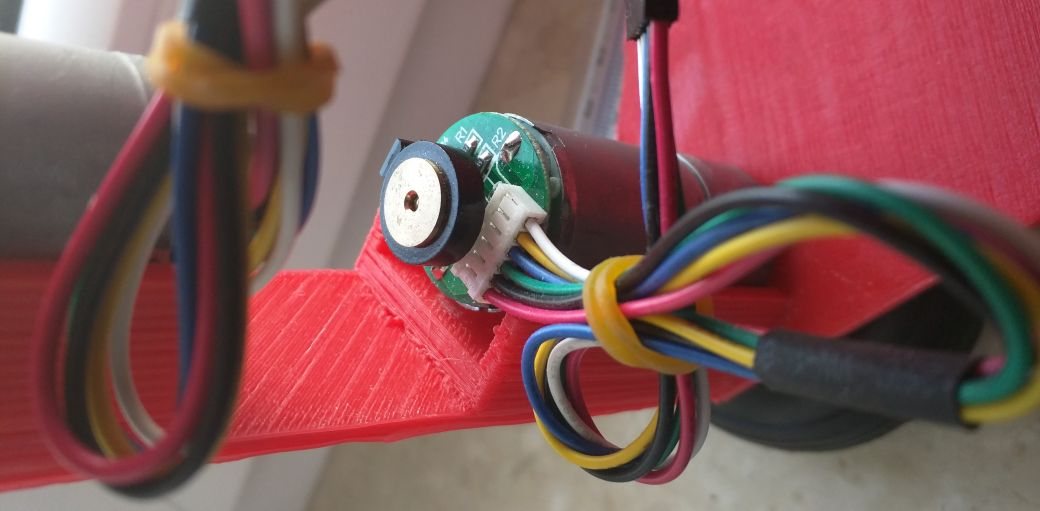
\includegraphics[scale=0.4]{\ImgPath/enkoder.jpg}
\end{center}
	\caption{Enkodery magnetyczne CPR 48 i wyprowadzenia przewodów silnika [opracowanie własne]}
	\label{schematKomunikacji}
\end{figure}

\noindent Wyprowadzenia silników:
\begin{itemize}
\item czerwony - zasilanie silnika 1,
\item czarny - zasilanie silnika 2,
\item zielony - potencjał masy enkodera,
\item niebieski - zasilanie enkodera, tolerancja od 3,5 V do 20 V,
\item żółty - wyjście A enkodera,
\item biały - wyjście B enkodera,
\end{itemize}

\noindent Wyjście B enkodera jest przesunięte w fazie o 90 stopni względem wyjścia A, co pozwala na ustalenie kierunku poruszania się kół \cite{pololu}.

\begin{figure}[!htbp]
	\begin{center}
\centering
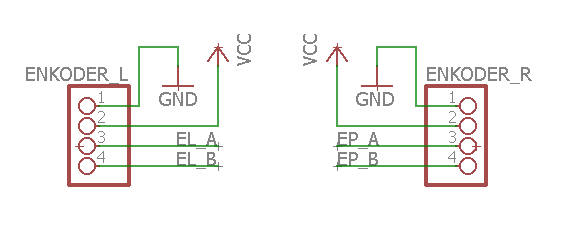
\includegraphics[scale=0.8]{\ImgPath/enkodery_sch.PNG}
\end{center}
	\caption{Sposób połączenia enkoderów w programie EAGLE [opracowanie własne]}
	\label{schematKomunikacji}
\end{figure}

\newpage

\subsection{Dwukanałowy mostek H - układ L298N}

Dwukanałowy mostek H pozwala sterować pracą dwóch silników prądu stałego w obu kierunkach przez mikrokontroler, którego wyjścia mają niską wydajność prądową. W projekcie został zastosowany układ scalony L298N o specyfikacji \cite{l298n}:
\begin{itemize}
\item Liczba kanałów: 2
\item Napięcie zasilania silników: maks. 46 V
\item Napięcie zasilania części logicznej: 4,5 V - 7 V
\item Szczytowy prąd na kanał: 2 A
\end{itemize}

\begin{figure}[!htbp]
	\begin{center}
\centering
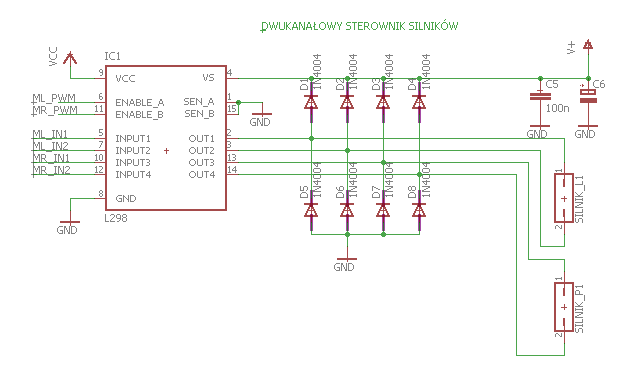
\includegraphics[scale=0.8]{\ImgPath/l298npol.PNG}
\end{center}
	\caption{Schemat połączenia układu L298N wykonany w programie EAGLE [opracowanie własne]}
	\label{schematKomunikacji}
\end{figure}

Sterowanie prędkością odbywa się za pomocą regulowania wypełnienia sygnału PWM na odpowiednich pinach. Natomiast sterowanie kierunkiem poruszania się poprzez wystawienie stanu wysokiego na wejściu IN1 oraz stanu niskiego na wejściu IN2 bądź odwrotnie.

Program sterownika silników za pomocą regulatora PID i sprzężenia zwrotnego w postaci odczytu położenia kół z enkoderów magnetycznych znajdujących się przy silnikach wystawia wartości zadane skorygowane o wyjście regulatora w postaci sygnału PWM na wejścia układu scalonego L298N.

Sam układ scalony L298N, nie w gotowym module, został zastosowany ze względu na niewielką cenę. Do prawidłowego działania należało jedynie dokupić, według noty katalogowej, 8 diod prostowniczych, 1 kondensator elektrolityczny \SI{100}{\micro F} i 1 kondensator ceramiczny 100 nF \cite{l298n}.

\begin{figure}[!htbp]
	\begin{center}
\centering
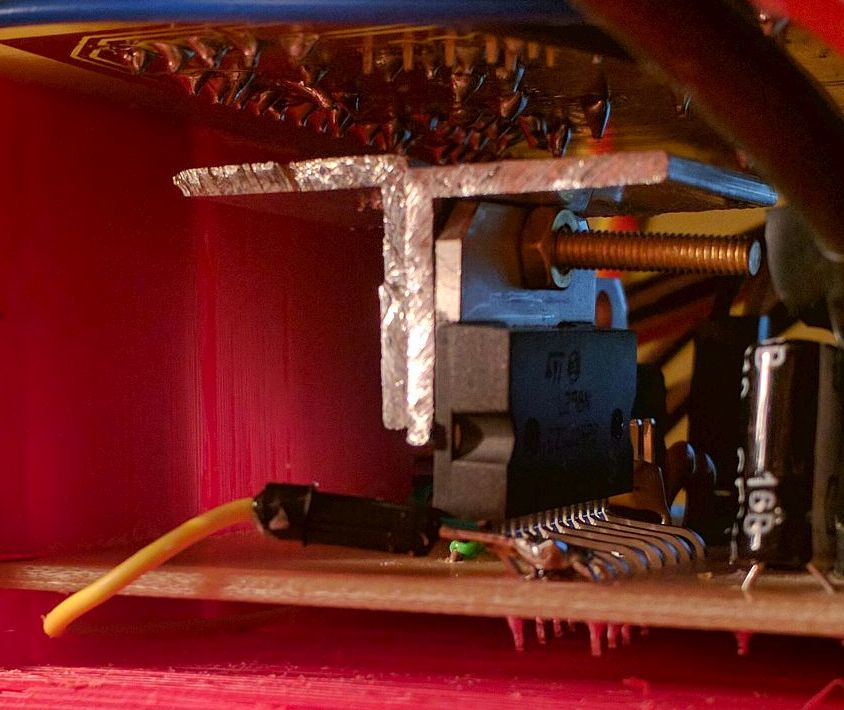
\includegraphics[scale=0.3]{\ImgPath/l298n.jpg}
\end{center}
	\caption{Układ scalony L298N z aluminiowymi radiatorami [opracowanie własne]}
	\label{schematKomunikacji}
\end{figure}

\subsection{Mikrokontroler z rodziny megaAVR}

Początkowo układ zasilający miał pełnić osobną funkcję sterownika silników, dlatego na płytce znajduje się 28-pinowa podstawka precyzyjna pod 8-bitowy mikrokontroler z rodziny megaAVR. W wyniku testowania układu to rozwiązanie stało się niewydajne i piny z podstawki zostały bezpośrednio połączone do płytki NUCLEO F103RB. Jednak daje to możliwość umieszczenia dodatkowego mikrokontrolera w razie potrzeby. Wszystkie elementy elektroniczne są przygotowane zgodnie z notami katalogowymi mikrokontrolerów firmy Atmel wraz z gniazdem do programowania o 10 pinowym standardzie KANDA \cite{atmega168}.

\begin{figure}[!htbp]
	\begin{center}
\centering
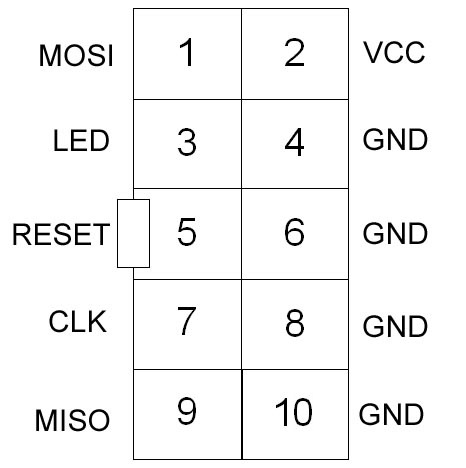
\includegraphics[scale=0.3]{\ImgPath/kanda.jpg}
\end{center}
	\caption{Schemat gniazda KANDA [opracowanie własne]}
	\label{schematKomunikacji}
\end{figure}

\begin{figure}[!htbp]
	\begin{center}
\centering
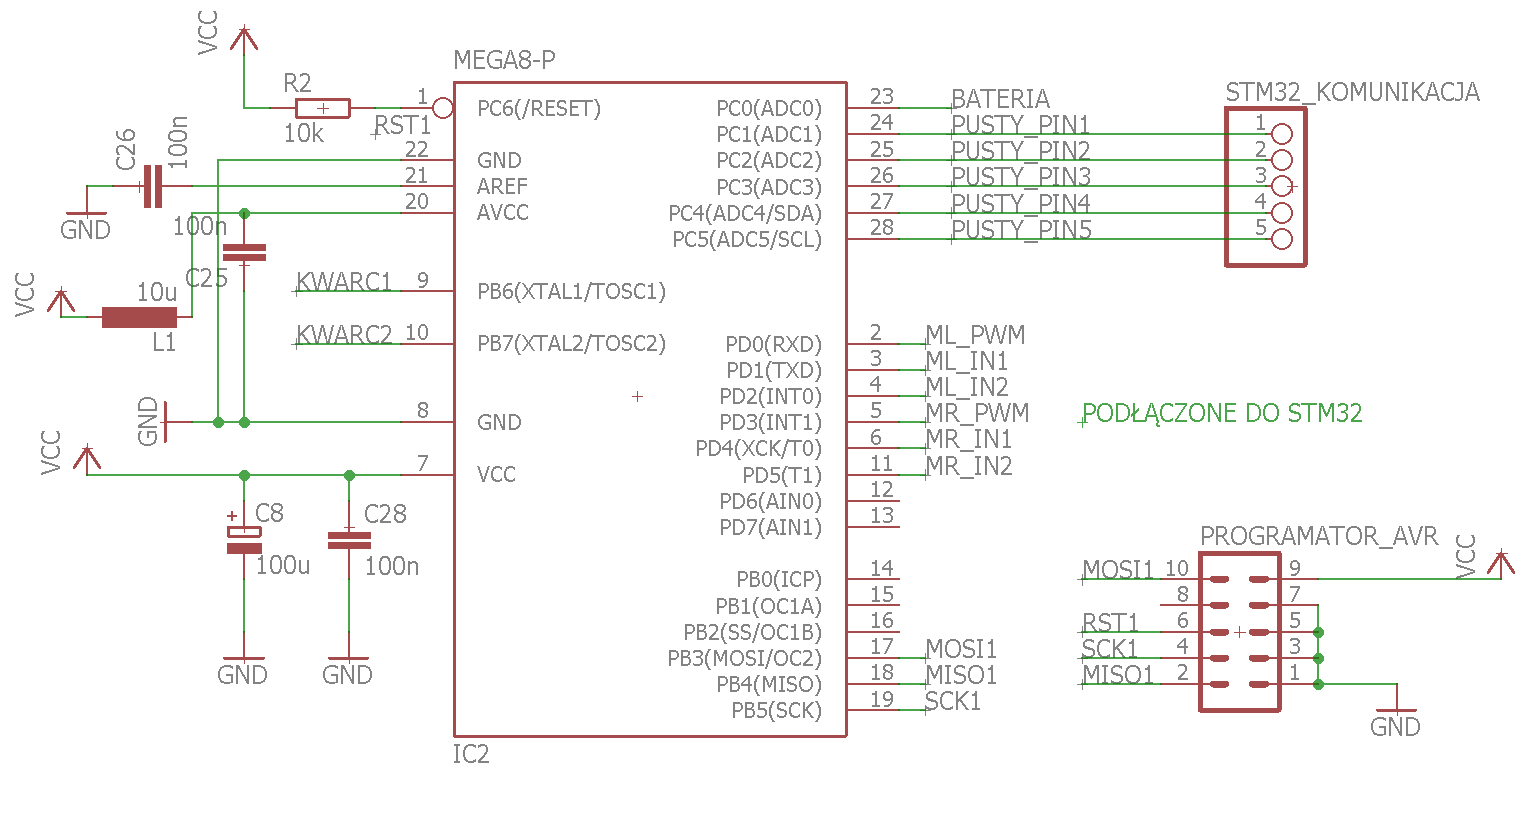
\includegraphics[scale=0.35]{\ImgPath/atmega168_sch.PNG}
\end{center}
	\caption{Schemat połączeń podstawki pod mikrokontroler z rodziny megaAVR w programie EAGLE [opracowanie własne]}
	\label{schematKomunikacji}
\end{figure}

\newpage
\subsection{Wykonanie płytki drukowanej}

Do wykonania płytki drukowanej - PCB (printed circuit board) został zaprojektowany schemat wszystkich połączeń w programie Autodesk EAGLE 8.3.1:

\begin{figure}[!htbp]
	\begin{center}
\centering
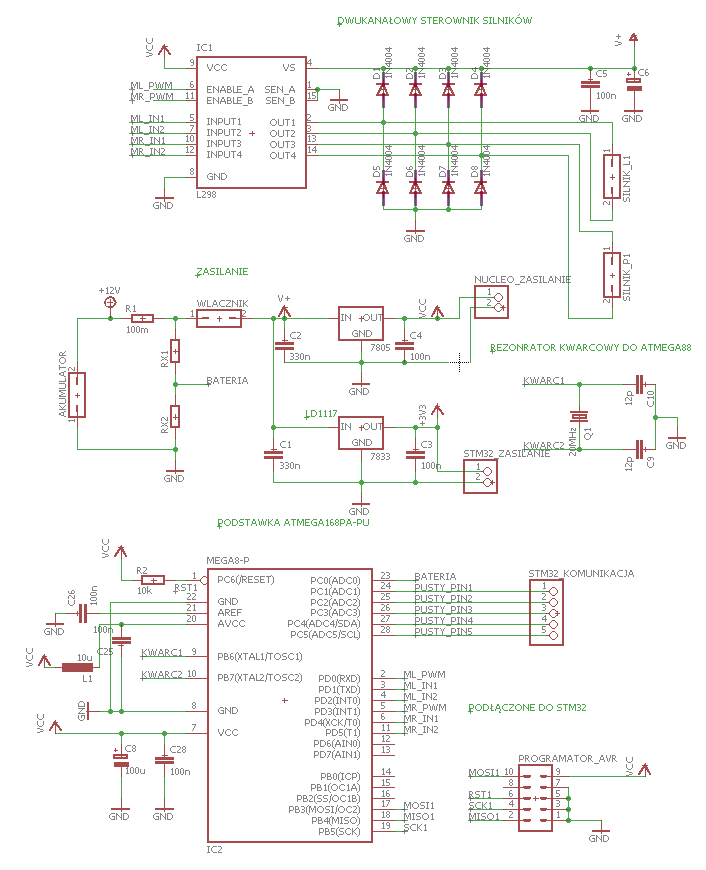
\includegraphics[scale=0.7]{\ImgPath/sterownik-silnikow_sch.PNG}
\end{center}
	\caption{Projekt połączeń elektronicznych układu zasilającego wykonany w programie EAGLE [opracowanie własne]}
	\label{schematKomunikacji}
\end{figure}

Oprócz schematu połączeń elementów elektronicznych, został również wykonany projekt PCB:

\begin{figure}[!htbp]
	\begin{center}
\centering
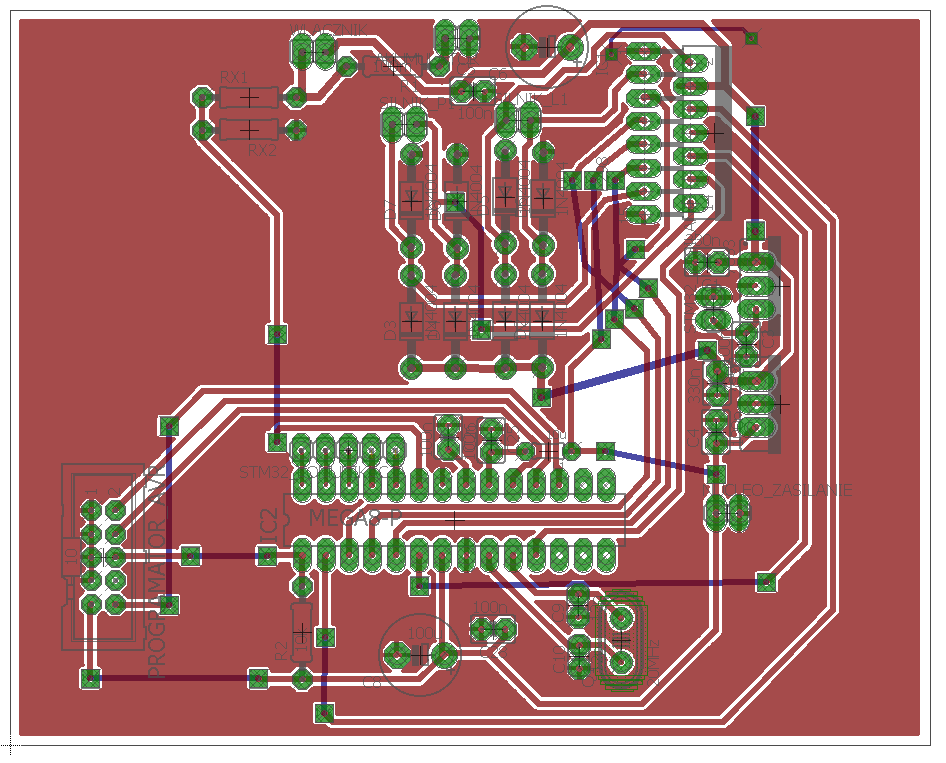
\includegraphics[scale=0.35]{\ImgPath/sterownik-silnikow_brd.PNG}
\end{center}
	\caption{Projekt PCB układu zasilającego wykonany w programie EAGLE [opracowanie własne]}
	\label{schematKomunikacji}
\end{figure}

\begin{figure}[!htbp]
	\begin{center}
\centering
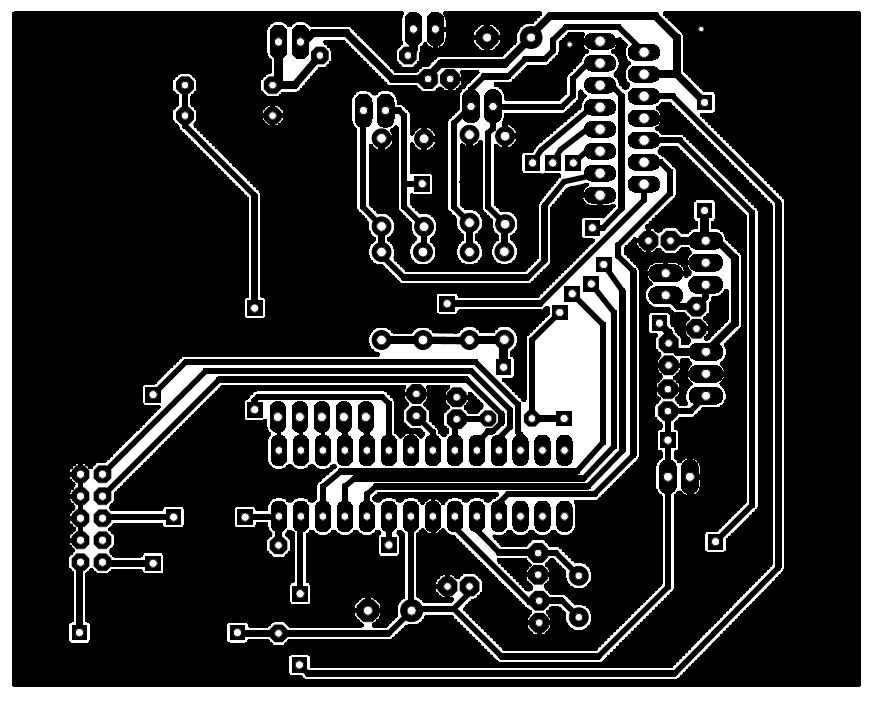
\includegraphics[scale=0.35]{\ImgPath/sterownik-silnikow_druk.PNG}
\end{center}
	\caption{Obraz połączeń elementów elektronicznych układu zasilającego przygotowany do wydrukowania [opracowanie własne]}
	\label{schematKomunikacji}
\end{figure}

\newpage
Projekt PCB został wyeksportowany do pliku PDF, aby uniknąć jakiegokolwiek przeskalowania elementów. Wydruk został przeprowadzony na drukarce laserowej na papierze kredowym. Wykorzystanie tego typu papieru umożliwia przeniesienie toneru na laminat pokryty miedzią za pomocą techniki termotransferu. Wydruk i papier zostały wyprasowane w temperaturze około 220 \textdegree C przez około 7 minut. Tak wysoka temperatura była konieczna ze względu na użytą płytkę pokrytą dwustronnie miedzią - większa ilość metalu pochłania więcej ciepła. Następnie wyprasowane elementy zostały zanurzone na 15 minut w wodzie, a po rozmiękczeniu papieru został on delikatnie usunięty z płytki. Po powyższych czynnościach został usunięty osiadły kamień za pomocą zwykłego noża, a także zostały poprawione wszelkie niedoskonałości powstałe podczas termotransferu. W pełni przygotowana płytka została poddana trawieniu w roztworze nadsiarczanu sodu przez ponad 30 minut, pozwoliło to na usunięcie miedzi z miejsc niepokrytych tonerem. Na koniec zostały wywiercone otwory do montażu elementów elektronicznych przewlekanych przy użyciu wiertła o średnicy 1 mm.

Po ukończeniu płytki, przewody i uprzednio przetestowane elementy elektroniczne zostały przylutowane. Po skończonym montażu elementów, wszystkie ścieżki zostały sprawdzone za pomocą multimetru, czy ciągłość obwodu jest zachowana tam, gdzie powinna, a także czy nie zachodzą zwarcia. Następnie został przylutowany akumulator i nastąpiła konieczność sprawdzenia wszystkich poziomów napięć na płytce. Po upewnieniu się, że wszystko jest wykonane prawidłowo płytka została przymocowana do obudowy robota.

\begin{figure}[!htbp]
	\begin{center}
\centering
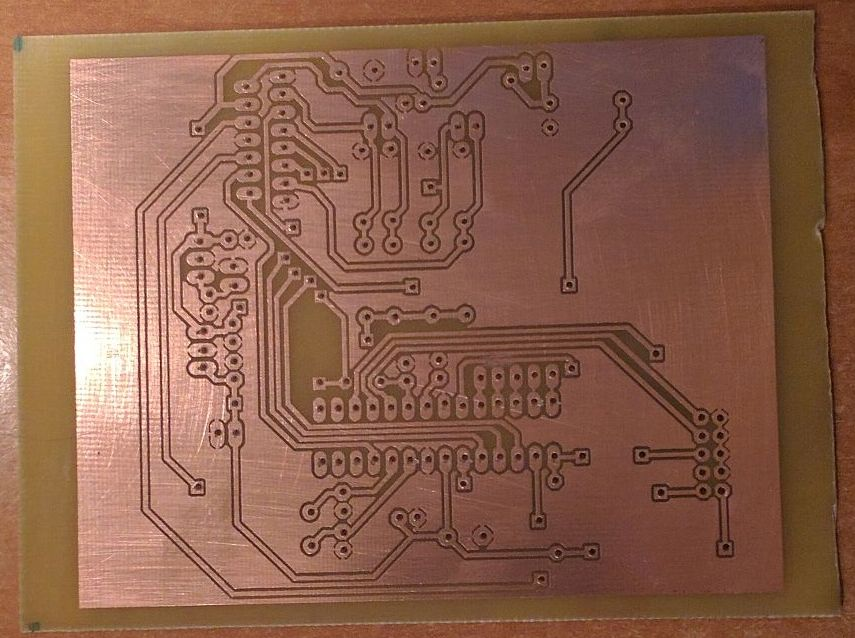
\includegraphics[scale=0.35]{\ImgPath/sterownikdcprzed.jpg}
\end{center}
	\caption{Płytka drukowana układu zasilającego wytrawiona w roztworze nadsiarczanu sodu [opracowanie własne]}
	\label{schematKomunikacji}
\end{figure}

\begin{figure}[!htbp]
	\begin{center}
\centering
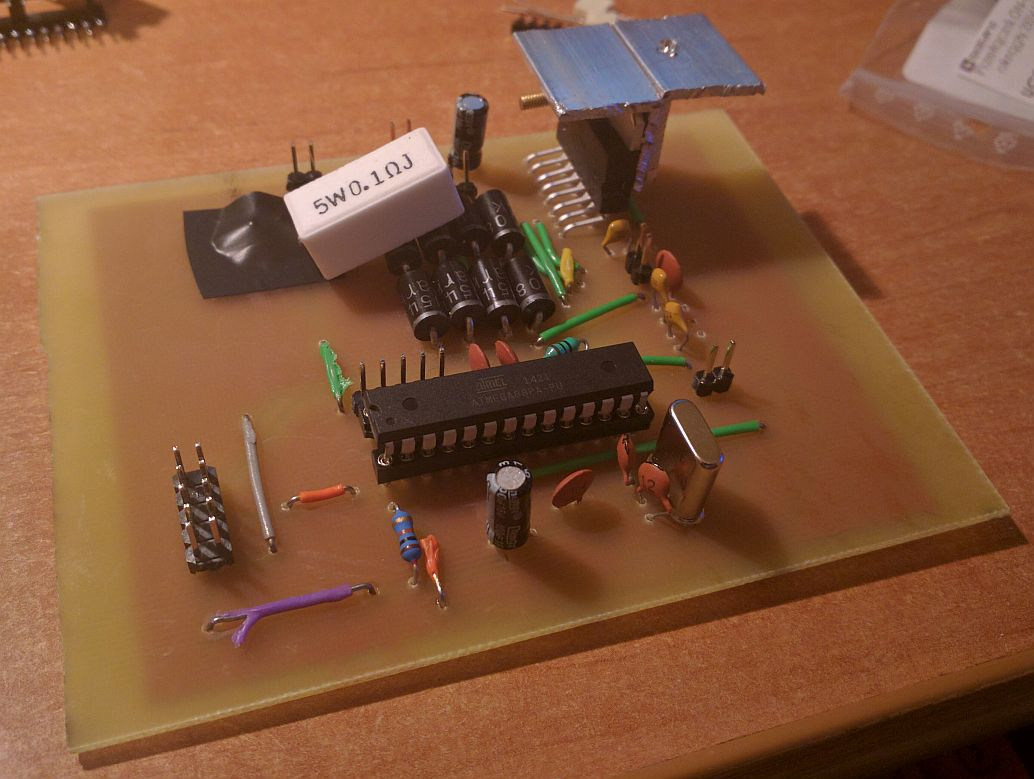
\includegraphics[scale=0.3]{\ImgPath/sterownikdcpo.jpg}
\end{center}
	\caption{Gotowa płytka układu zasilającego [opracowanie własne]}
	\label{schematKomunikacji}
\end{figure}

\newpage

  %-----------------
  % Układ sterujący
  %-----------------
\section{Układ sterujący}

Do wykonywania wszystkich obliczeń został wybrany mikrokontroler\\ STM32F103RBT6 na płytce NUCLEO F103RB. Układ scalony zbiera informacje ze wszystkich czujników robota: enkoderów magnetycznych, akcelerometru, żyroskopu, czujników ultradźwiękowych i modułu Wi-Fi. Następnie wykorzystuje te dane do obliczenia aktualnej prędkości i kierunku obrotów silników, aby utrzymać pion i wysłać dane przez interfejs USART do modułu Wi-Fi.
Przeprogramowywanie mikrokontrolera jest ułatwione poprzez wbudowany programator na płytce NUCLEO i wywiercony otwór w obudowie na wtyk USB.

\begin{figure}[!htbp]
	\begin{center}
\centering
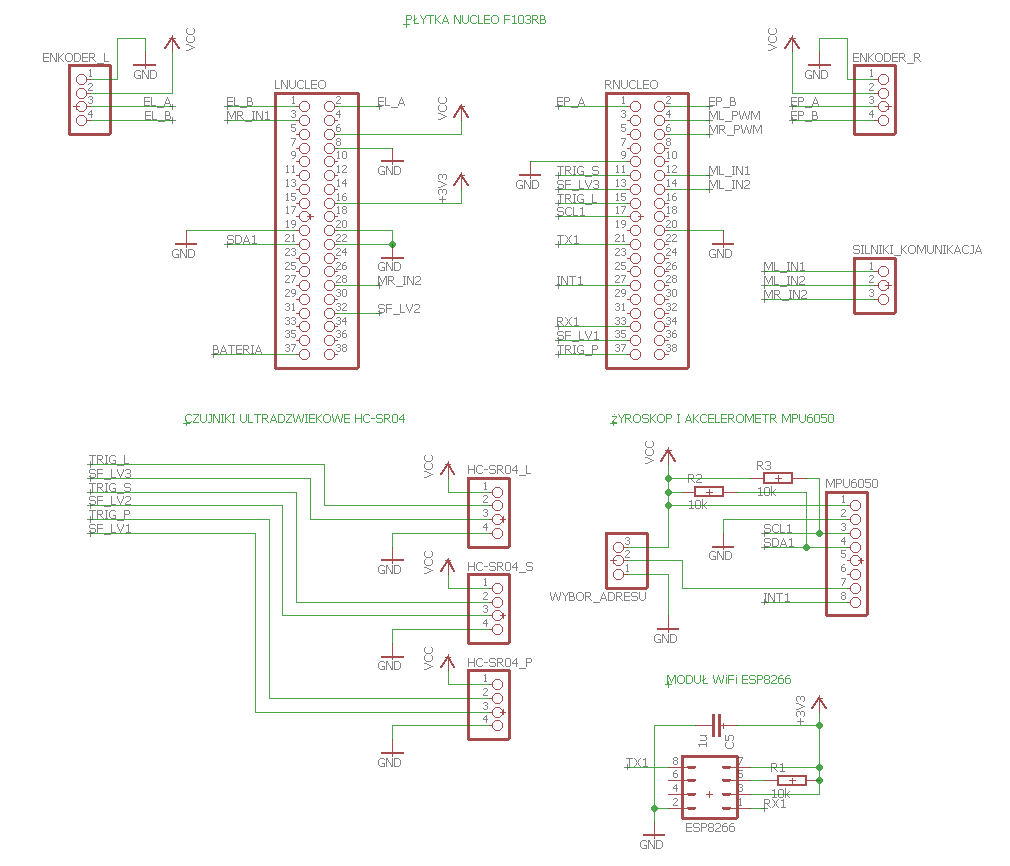
\includegraphics[scale=0.5]{\ImgPath/sterowanie_sch.PNG}
\end{center}
	\caption{Sposób połączenia elementów elektronicznych układu sterującego wykonany w programie EAGLE [opracowanie własne]}
	\label{schematKomunikacji}
\end{figure}

\newpage

\newpage

\subsection{Mikrokontroler STM32F103RBT6}

Mikrokontroler STM32F103RBT6 32-bitowej architektury ARM na płytce NUCLEO z wyprowadzeniami pinów układu scalonego na złącza goldpin i zintegrowany z programatorem został wybrany ze względu na łatwość montażu i programowania. Architektura używanego mikrokontrolera jest oprarta na rdzeniu Cortex M3, co przekłada się na wysoki stosunek mocy obliczeniowej do ceny - dane techniczne \cite{nucleo,stm32datasheet}:
\begin{itemize}
\item częstotliwość taktowania: 72 MHz,
\item pamięć flash: 128 kB,
\item pamięć SRAM: 20 kB,
\item 2 przetworniki analogowo-cyfrowe 12-bitowe, 16-kanałowe,
\item 7 liczników (timer),
\item interfejsy: 3 USART, 2 SPI 18 Mbit/s, 2 I2C, USB Full Speed, CAN 2,0B,
\item debugger ST-Link/V2 umieszczony na płytce,
\end{itemize}

\begin{figure}[!htbp]
	\begin{center}
\centering
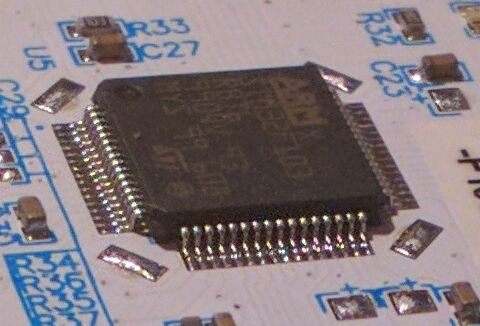
\includegraphics[scale=0.3]{\ImgPath/stm32.jpg}
\end{center}
	\caption{Mikrokontroler STM32F103RBT6 w obudowie LQFP64 [opracowanie własne]}
	\label{schematKomunikacji}
\end{figure}

\begin{figure}[!htbp]
	\begin{center}
\centering
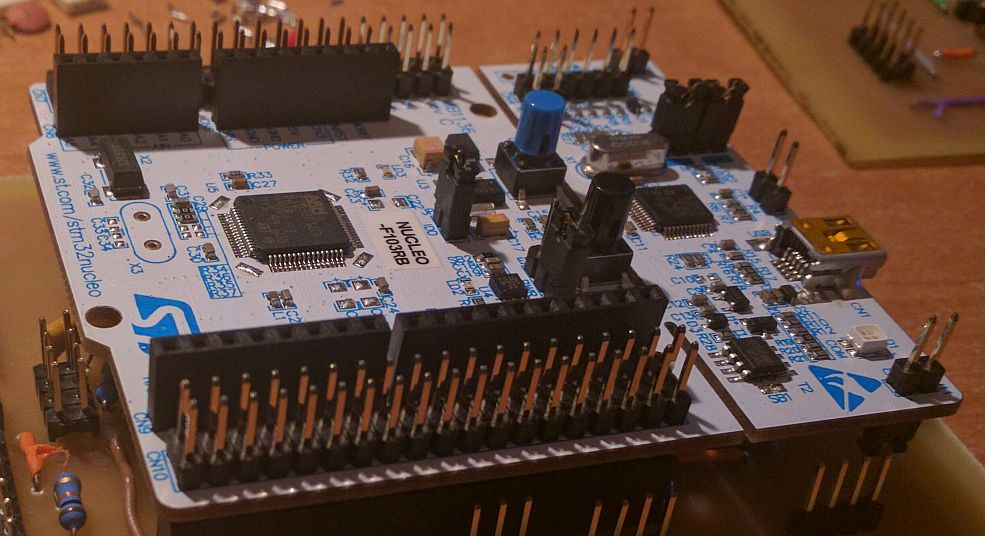
\includegraphics[scale=0.4]{\ImgPath/nucleo.jpg}
\end{center}
	\caption{Płytka NUCLEO-F103RB [opracowanie własne]}
	\label{schematKomunikacji}
\end{figure}

\begin{figure}[!htbp]
	\begin{center}
\centering
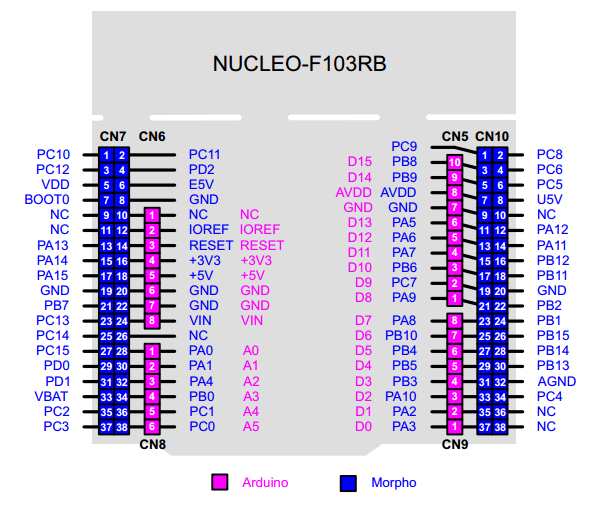
\includegraphics[scale=0.7]{\ImgPath/f103rb.PNG}
\end{center}
	\caption{Wyprowadzenia NUCLEO-F103RB [źródło: \cite{nucleo}, strona 30]}
	\label{schematKomunikacji}
\end{figure}

\newpage

Mikrokontroler jest programowany przez złącze Mini USB znajdujące się na płytce. Układ scalony STM32F103RBT6 jest wykorzystywany do zbierania sygnałów ze wszystkich czujników:
\begin{itemize}
\item enkodery magnetyczne - sprzężenie zwrotne w postaci informacji o położeniu kół do układu regulacji położenia w pionie i sterownika silników,
\item akcelerometr i żyroskop - sprzężenie zwrotne w postaci informacji o przyspieszeniu kątowym i kącie pochylenia robota do układu sterowania,
\item czujniki ultradźwiękowe - informacje o położeniu przeszkód na drodze - do układu skanowania pomieszczeń,
\item moduł Wi-Fi - odbieranie rozkazów wysyłanych za pośrednictwem aplikacji internetowej.
\end{itemize}

Zadaniem mikrokontrolera jest przede wszystkim wykorzystać informacje o przebytej drodze i pochyleniu robota do utrzymania pozycji pionowej za pomocą kaskady regulatorów PID. Sygnały z czujników jako zmienne stanu dodatkowo przechodzą przez filtry: cyfrowy dolnoprzepustowy, cyfrowy górnoprzepustowy i zostają uśredniane, co znacząco zwiększa ich dokładność. Drugim zadaniem układu scalonego jest zebranie informacji o aktualnym stanie pomieszczenia (odległości od wszystkich obiektów dookoła robota) oraz wysłanie ich przez moduł Wi-Fi i sieć lokalną (co może być odebrane przez dowolne urządzenie obsługujące protokół HTTP i znające adres IP modułu ESP8266 w tej sieci). Po każdorazowym wykonaniu czynności obliczone wartości prędkości i kierunku obrotu kół są wysyłane do sterownika silników.\\
Połączenie płytki NUCLEO z resztą układu nie wymagało żadnych dodatkowych elementów pasywnych lub aktywnych.

\begin{figure}[!htbp]
	\begin{center}
\centering
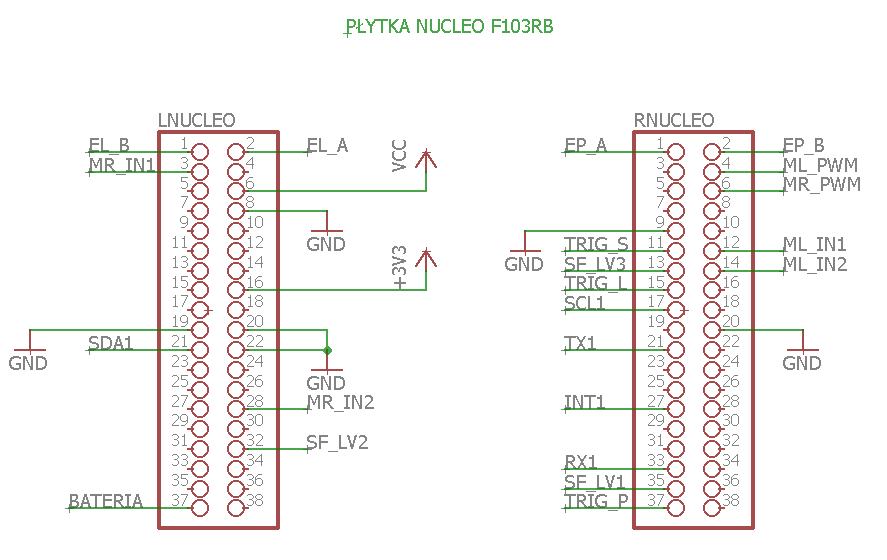
\includegraphics[scale=0.5]{\ImgPath/nucleo_sch.PNG}
\end{center}
	\caption{Schemat połączeń płytki NUCLEO F103RB wykonany w programie EAGLE [opracowanie własne]}
	\label{schematKomunikacji}
\end{figure}

\newpage

\subsection{Żyroskop i akcelerometr - układ MPU6050}

Użyty moduł firmy Invensense zawiera wbudowany cyfrowy żyroskop i akcelerometr. Jego zastosowanie wynika z niskiej ceny i dostatecznych parametrów pracy \cite{mpu}:
\begin{itemize}
\item napięcie zasilania: 3,3 V - 5 V,
\item zakresy pracy żyroskopu: 250 \textdegree/s, 500 \textdegree/s, 1000 \textdegree/s, 2500 \textdegree/s,
\item zakresy pracy akcelerometru: 2 g, 4 g, 8 g, 16 g (1 g to około 9,81 m/s$^2$),
\item wymiary: 20 mm x 16 mm,
\item waga: 0,9 g.
\end{itemize}

\begin{figure}[!htbp]
	\begin{center}
\centering
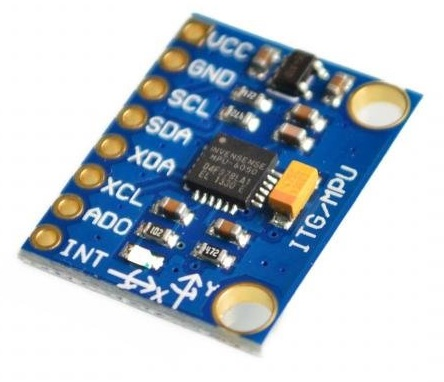
\includegraphics[scale=0.25]{\ImgPath/mpu_zdj.jpg}
\end{center}
	\caption{Żyroskop i akcelerometr - układ MPU6050 \cite{mpuallegro}}
	\label{schematKomunikacji}
\end{figure}

Komunikacja z modułem odbywa się za pośrednictwem magistrali szeregowej I2C. Ścieżki SDA i SCL zostały podciągnięte do napięcia zasilania, aby uniknąć stanów nieokreślonych na pinach. 

\begin{figure}[!htbp]
	\begin{center}
\centering
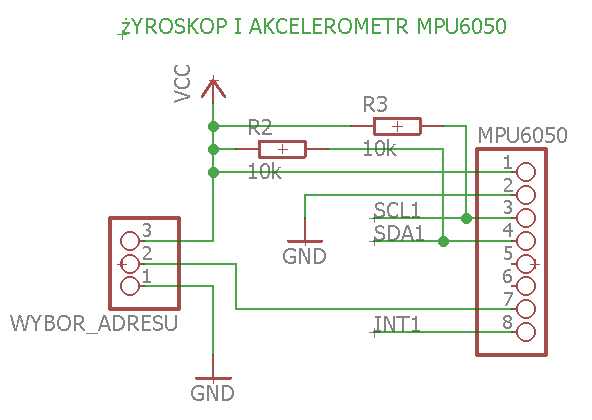
\includegraphics[scale=0.55]{\ImgPath/mpue.PNG}
\end{center}
	\caption{Sposób połączenia czujnika MPU6050 wykonany w programie EAGLE [opracowanie własne]}
	\label{schematKomunikacji}
\end{figure}

\begin{figure}[!htbp]
	\begin{center}
\centering
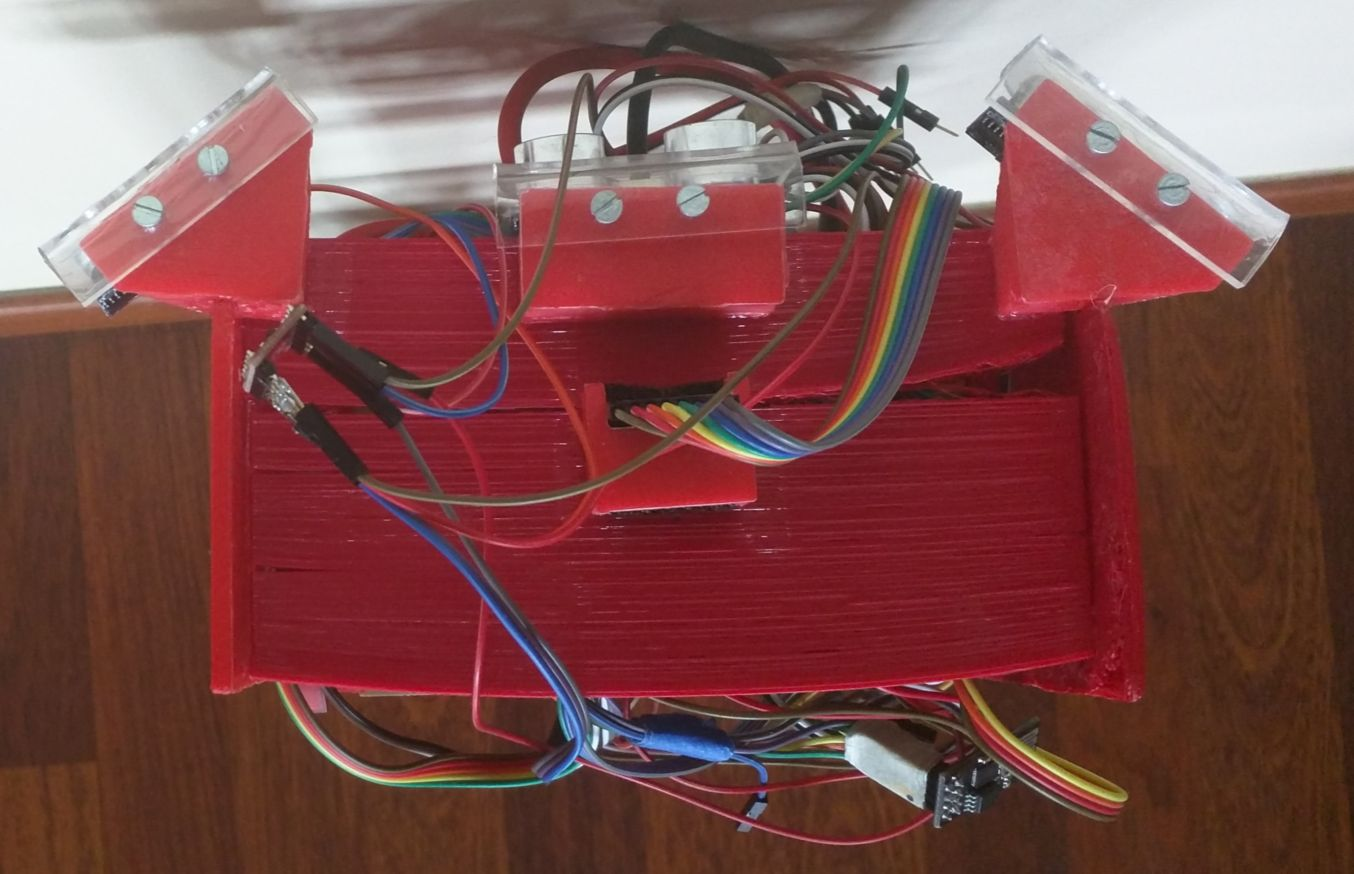
\includegraphics[scale=0.3]{\ImgPath/mpuumieszczenie.jpg}
\end{center}
	\caption{Umiejscowienie czujnika MPU6050 na obudowie robota [opracowanie własne]}
	\label{schematKomunikacji}
\end{figure}

\subsection{Czujniki ultradźwiękowe HC-SR04}

Użyte czujniki HC-SR04 zostały zakupione razem z uchwytami montażowymi. Ich zastosowanie wynika z niskiej ceny i dostatecznych parametrów pracy \cite{hcsr04}:
\begin{itemize}
\item napięcie zasilania: 5 V,
\item średni pobór prądu: 15 mA,
\item zakres pomiarowy: od 2 cm do 400 cm,
\item częstotliwość pracy: 40 kHz,
\item wymiary: 45 mm x 20 mm x 15 mm.
\end{itemize}

\begin{figure}[!htbp]
	\begin{center}
\centering
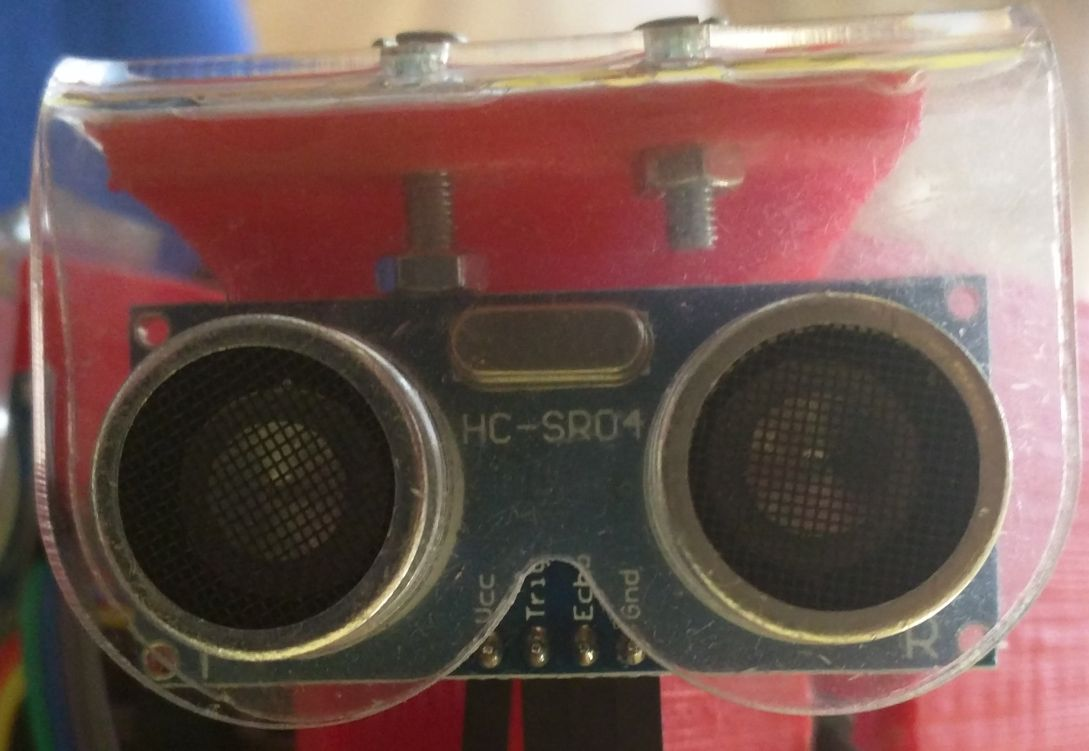
\includegraphics[scale=0.2]{\ImgPath/hcsr04.jpg}
\end{center}
	\caption{Czujniki ultradźwiękowe HC-SR04 [opracowanie własne]}
	\label{schematKomunikacji}
\end{figure}

Komunikacja z czujnikami odbywa się za pośrednictwem dwóch pinów: ECHO i TRIG. Wynika to z działania układu - aby rozpocząć pomiar należy podać na pin TRIG impuls napięciowy (stan wysoki 5V) przez \SI{10}{\micro s}. Moduł dokonuje pomiaru odległości przy pomocy fali dźwiękowej o częstotliwości 40 kHz. Na pinie ECHO otrzymywany jest sygnał, w którym odległość od przeszkody jest zależna od czasu trwania stanu wysokiego. Odległość w centymetrach od przeszkody wynosi:\\
\\
\noindent Wzór 3.1: $d = 0,017t_{ECHO}$,\\
gdzie:\\
$d$ - odległość mierzona,\\
$t_{echo}$ - czas trwania stanu wysokiego na pinie ECHO.

\newpage
\noindent Wzór jest wyprowadzony z prostej zależności:\\
Wzór 3.2: $d = (t_{echo}V_{sound})/2$,\\
gdzie:\\
$V_{sound}$ - prędkość rozchodzenia się dźwięku w powietrzu - 340 m/s.

\begin{figure}[!htbp]
	\begin{center}
\centering
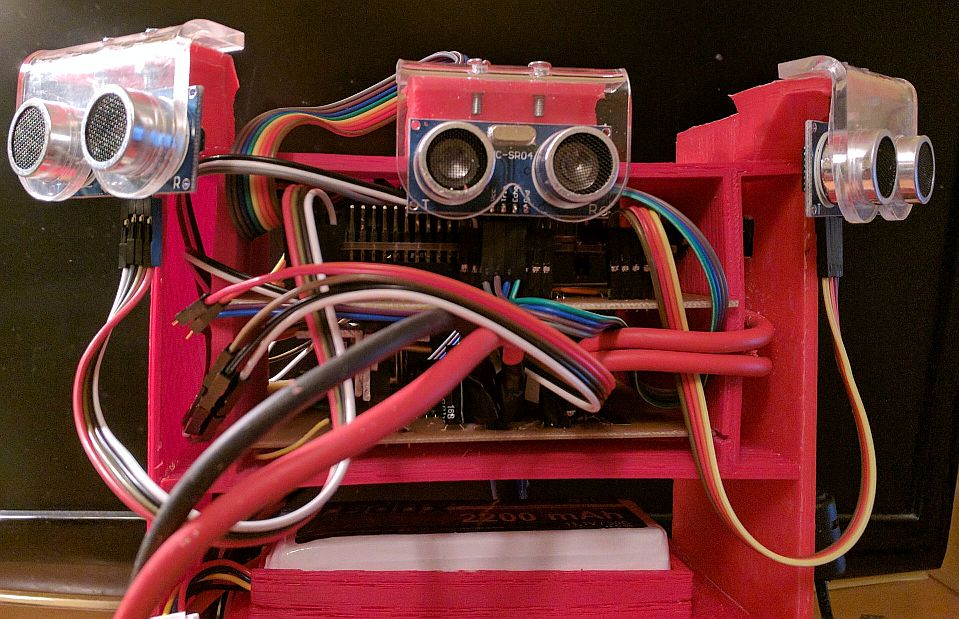
\includegraphics[scale=0.4]{\ImgPath/hcsrumieszczenie.jpg}
\end{center}
	\caption{Umieszczenie czujników HC-SR04 na obudowie robota [opracowanie własne]}
	\label{schematKomunikacji}
\end{figure}

W zestawie znajdują się specjalne uchwyty montażowe, do których zostały zaprojektowane mocowania na szczycie konstrukcji robota. Model w 3D został zaprojektowany w ten sposób, aby czujniki ultradźwiękowe były ustawione: idealnie na wprost jazdy, pod kątem 45\textdegree w prawo i 45\textdegree w lewo. Czujnik najlepiej działa w polu do 30\textdegree od osi prostopadłej do modułu. Stąd od odległości ok. 24 cm od konstrukcji robot będzie miał widoczność w pełnym zakresie 180\textdegree [Rysunek 3.30].

\begin{figure}[!htbp]
	\begin{center}
\centering
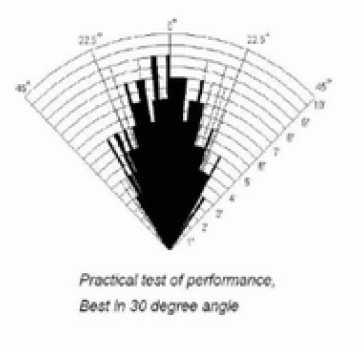
\includegraphics[scale=0.6]{\ImgPath/hcsrzasieg.PNG}
\end{center}
	\caption{Zasięg czujnika HC-SR04 [źródło: \cite{hcsr04}, strona 5]}
	\label{schematKomunikacji}
\end{figure}

\begin{figure}[!htbp]
	\begin{center}
\centering
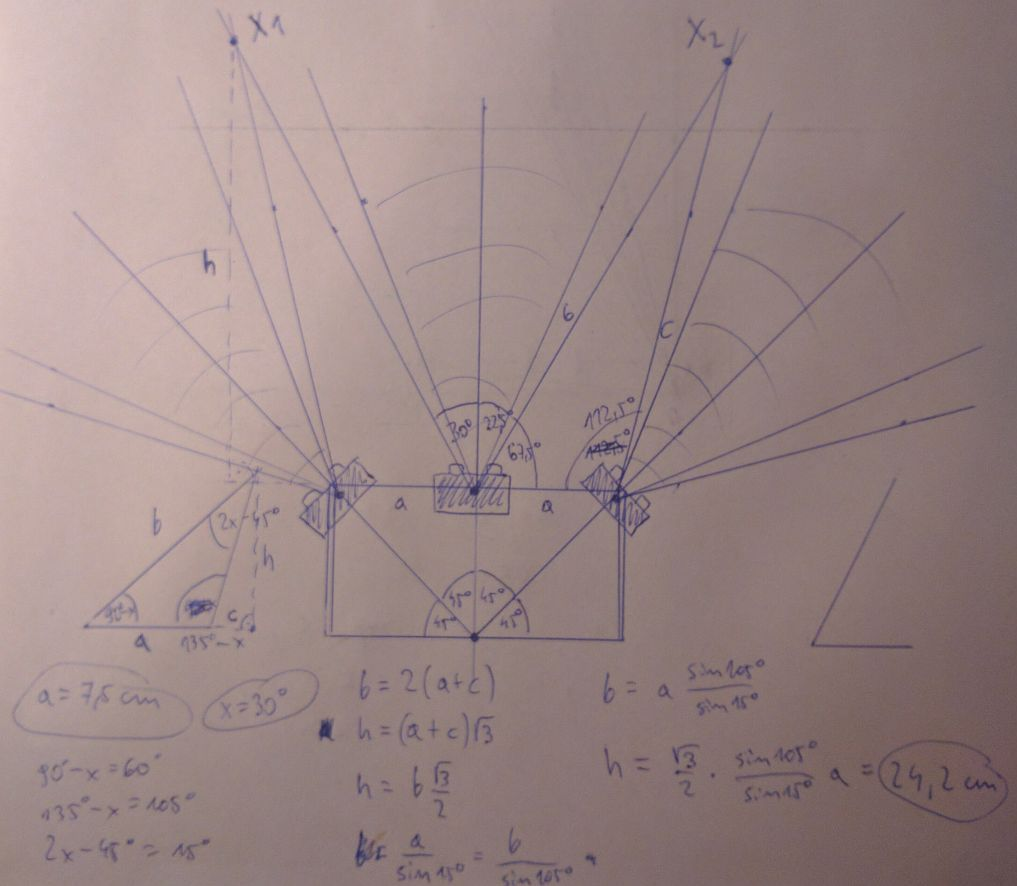
\includegraphics[scale=0.3]{\ImgPath/widocznosc.jpg}
\end{center}
	\caption{Obliczenie obszaru widoczności robota [opracowanie własne]}
	\label{schematKomunikacji}
\end{figure}

\begin{figure}[!htbp]
	\begin{center}
\centering
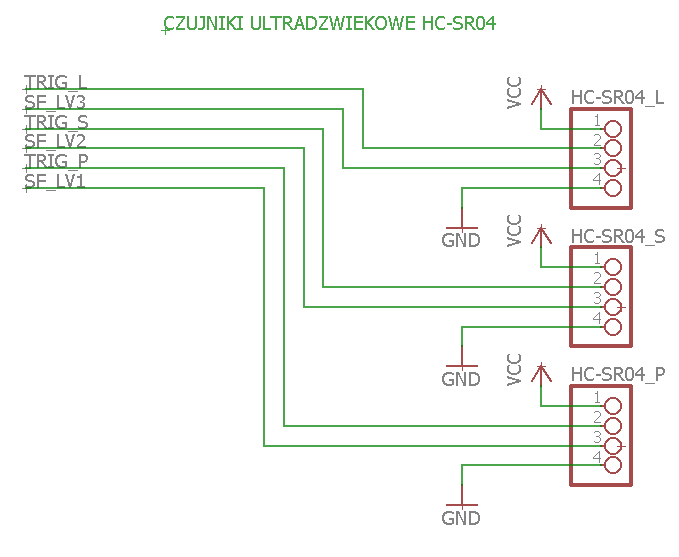
\includegraphics[scale=0.5]{\ImgPath/hcsr04_sch.PNG}
\end{center}
	\caption{Sposób połączenia czujników HC-SR04 wykonany w programie EAGLE [opracowanie własne]}
	\label{schematKomunikacji}
\end{figure}

\newpage

W związku z tym, że czujniki ultradźwiękowe HC-SR04 działają na napięciu 5 V, a mikrokontroler STM32F103RBT6 na napięciu 3,3 V, został zastosowany konwerter poziomów logicznych - TTL (napięć) firmy SparkFun. Testy na module wykazały, że piny TRIG mogą być wyzwalane napięciem 3,3 V, więc tylko piny ECHO zostały podłączone do mikrokontrolera poprzez konwerter napięć, aby zapobiec jego uszkodzeniu.

\begin{figure}[!htbp]
	\begin{center}
\centering
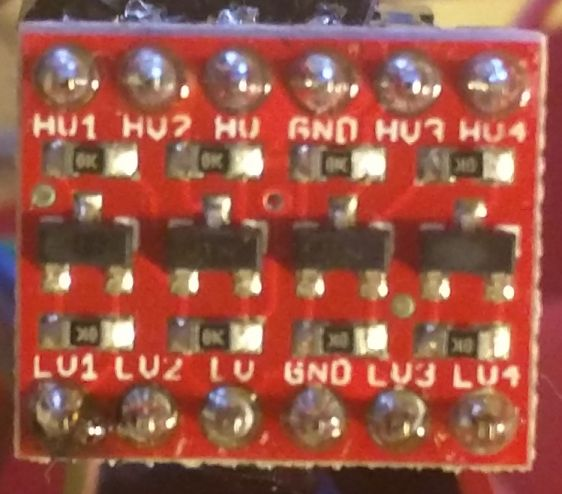
\includegraphics[scale=0.2]{\ImgPath/konwerter_zdj.jpg}
\end{center}
	\caption{Konwerter poziomów logicznych SparkFun [opracowanie własne]}
	\label{schematKomunikacji}
\end{figure}

\begin{figure}[!htbp]
	\begin{center}
\centering
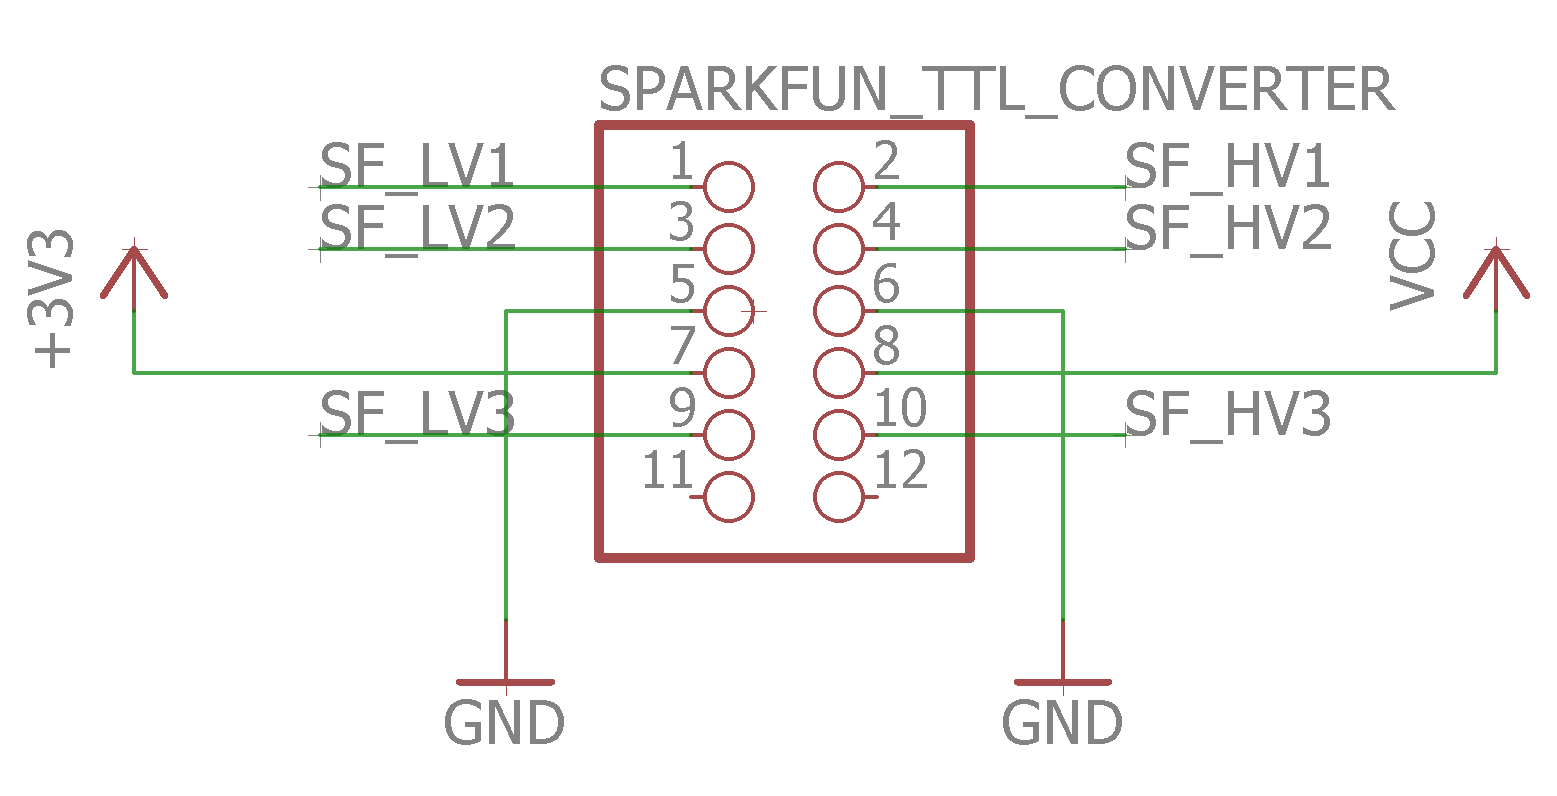
\includegraphics[scale=0.2]{\ImgPath/konwerter_sch.PNG}
\end{center}
	\caption{Schemat połączeń konwertera napięć logicznych SparkFun w programie EAGLE [opracowanie własne]}
	\label{schematKomunikacji}
\end{figure}

\newpage

\subsection{Moduł Wi-Fi ESP-01 8266}

Moduł został wybrany ze względu na niską cenę, powszechne użycie i du żą moc obliczeniową. Dane techniczne \cite{esp}:
\begin{itemize}
\item zasilanie: 3,3 V,
\item pamieć flash: 1 MB,
\item 2 GPIO - wyjścia/wejścia cyfrowe,
\item 1 UART,
\item wbudowana antena PCB,
\item wymiary: 24,8 mm x 16 mm.
\end{itemize}

\begin{figure}[!htbp]
	\begin{center}
\centering
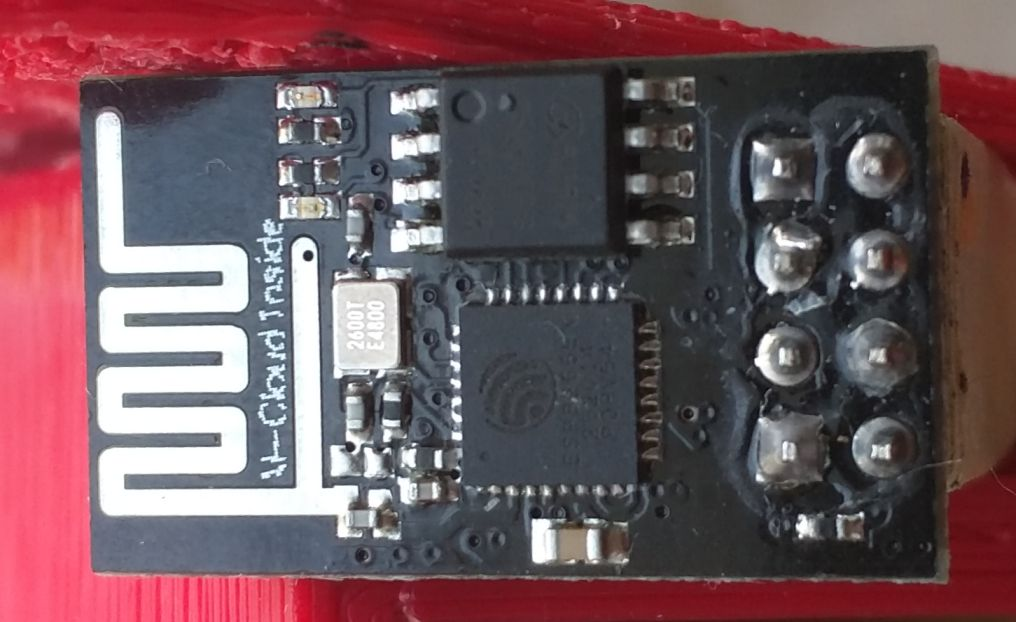
\includegraphics[scale=0.17]{\ImgPath/esp.jpg}
\end{center}
	\caption{Moduł Wi-Fi ESP-01 8266 [opracowanie własne]}
	\label{schematKomunikacji}
\end{figure}

\newpage
Komunikacja z modułem odbywa się za pośrednictwem interfejsu UART - piny RX i TX. Do prawidłowego działania układu został dołączony kondensator ceramiczny \SI{1}{\micro F} między napięcie zasilania a masę. Piny Reset i CH\_PD zostały podciągnięte do napięcia zasilania modułu, aby dodatkowo ustabilizować pracę urządzenia.

\begin{figure}[!htbp]
	\begin{center}
\centering
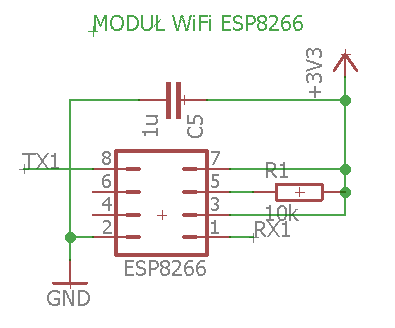
\includegraphics[scale=0.6]{\ImgPath/espe.PNG}
\end{center}
	\caption{Sposób połączenia modułu ESP8266 wykonany w programie EAGLE [opracowanie własne]}
	\label{schematKomunikacji}
\end{figure}

\begin{figure}[!htbp]
	\begin{center}
\centering
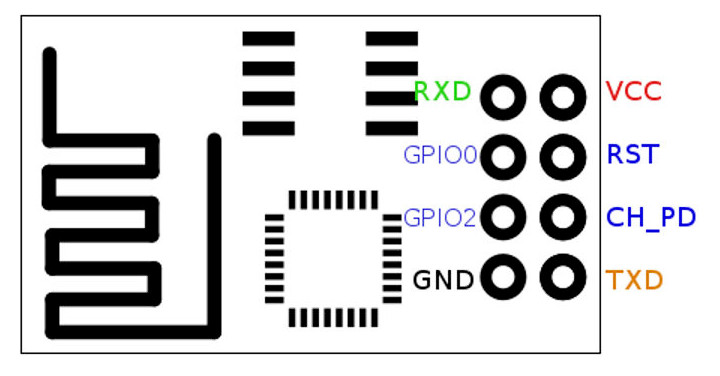
\includegraphics[scale=0.25]{\ImgPath/esp01.jpg}
\end{center}
	\caption{Wyprowadzenia ESP-01 8266 [opracowanie własne]}
	\label{schematKomunikacji}
\end{figure}

Do zaprogramowania modułu należy użyć pinów UART i zewrzeć pin GPIO0 do masy. Z powodu napięcia zasilania ESP8266 3,3 V konieczne jest zastosowanie konwertera napięć, aby podłączyć moduł przez interfejs USB do komputera PC. W tym wypadku został użyty konwerter UART-USB oparty na układzie PL2303, który może pracować na dwóch napięciach 3,3 V i 5 V (wybór napięcia za pomocą zworki).

\newpage
Do ESP8266 został wgrany firmware NodeMCU w wersji: nodemcu\_float\_0.9.6-dev\_20150704 za pomocą programu ESP8266Flasher. Nowy firmware umożliwia programowanie modułu za pomocą języka skryptowego Lua, a także w środowisku Arduino, z wykorzystaniem biblioteki esp8266 by ESP8266 Community w wersji 2.3.0-rc2

\begin{figure}[!htbp]
	\begin{center}
\centering
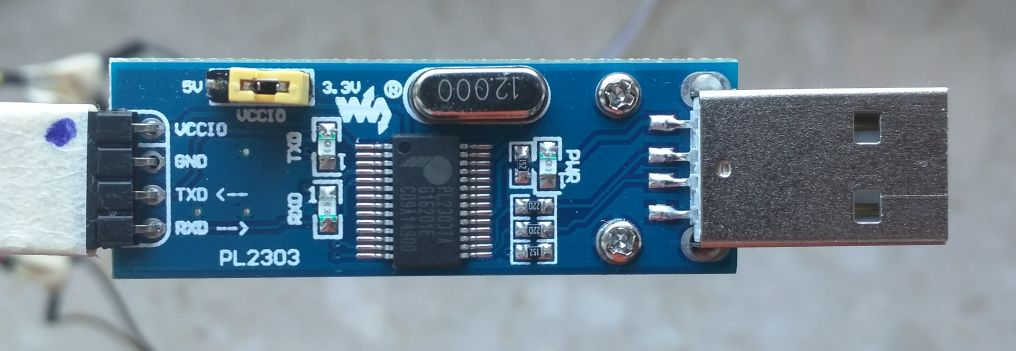
\includegraphics[scale=0.25]{\ImgPath/konwerter.jpg}
\end{center}
	\caption{Konwerter UART-USB oparty na układzie PL2303 [opracowanie własne]}
	\label{schematKomunikacji}
\end{figure}

\subsection{Wykonanie płytki drukowanej}

Płytka drukowana (PCB) układu sterującego została wykonana w analogiczny sposób jak płytka układu zasilającego. Zamiast podstawki precyzyjnej pod mikrokontroler zostały zamontowane żeńskie gniazda goldpin, w których można umieścić płytkę NUCLEO-F103RB.

\begin{figure}[!htbp]
	\begin{center}
\centering
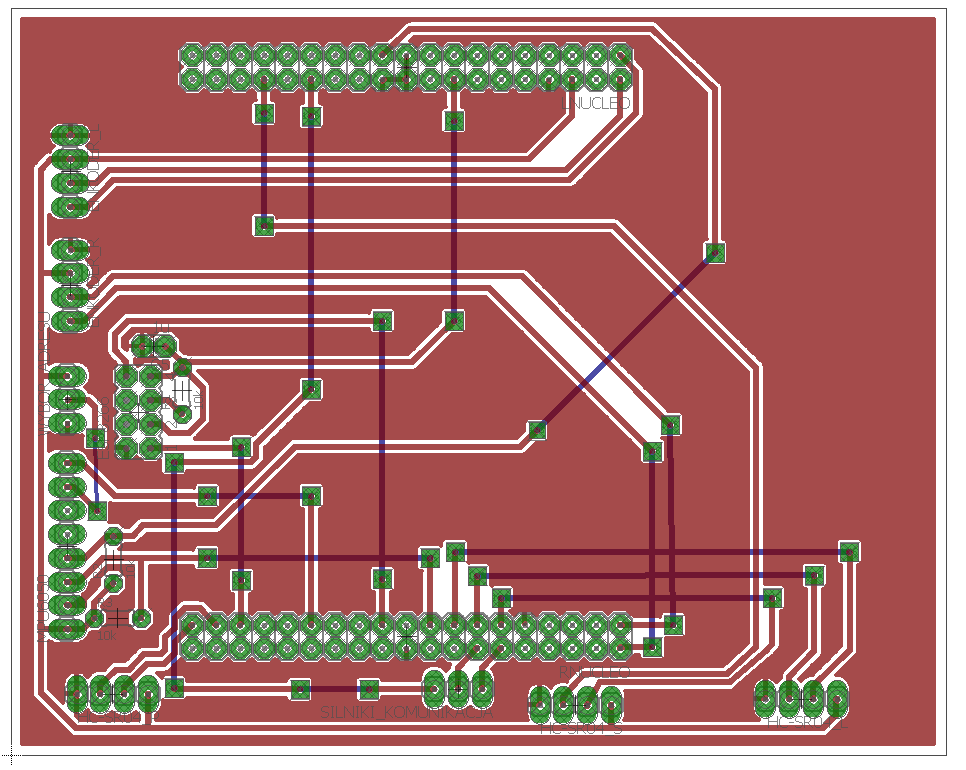
\includegraphics[scale=0.3]{\ImgPath/sterowanie_brd.PNG}
\end{center}
	\caption{Projekt PCB układu sterującego wykonany w programie EAGLE [opracowanie własne]}
	\label{schematKomunikacji}
\end{figure}

\begin{figure}[!htbp]
	\begin{center}
\centering
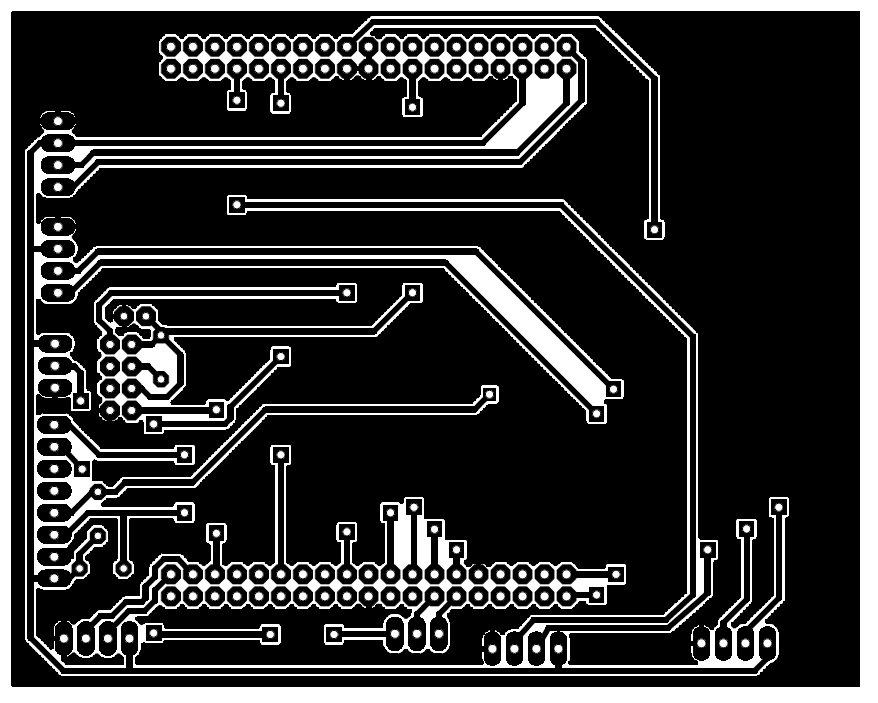
\includegraphics[scale=0.4]{\ImgPath/sterowanie_druk.PNG}
\end{center}
	\caption{Obraz połączeń elementów elektronicznych układu sterującego przygotowany do wydrukowania [opracowanie własne]}
	\label{schematKomunikacji}
\end{figure}

\begin{figure}[!htbp]
	\begin{center}
\centering
\includegraphics[scale=0.35]{\ImgPath/sterowanie1.jpg}
\end{center}
	\caption{Płytka drukowana układu sterującego wytrawiona w roztworze nadsiarczanu sodu [opracowanie własne]}
	\label{schematKomunikacji}
\end{figure}

\begin{figure}[!htbp]
	\begin{center}
\centering
\includegraphics[scale=0.35]{\ImgPath/sterowanie2.jpg}
\end{center}
	\caption{Gotowa płytka układu sterującego bez zamontowanej płytki NUCLEO-F103RB [opracowanie własne]}
	\label{schematKomunikacji}
\end{figure}

\begin{figure}[!htbp]
	\begin{center}
\centering
\includegraphics[scale=0.35]{\ImgPath/sterowanie3.jpg}
\end{center}
	\caption{Gotowa płytka układu sterującego z zamontowaną płytką NUCLEO-F103RB [opracowanie własne]}
	\label{schematKomunikacji}
\end{figure}

\newpage

%-----------------
% Teoria sterowania
%-----------------
\chapter{Teoria sterowania}

\section{Układ sterowania położenia w pionie}

Układ sterowania położenia w pionie składa się z dwóch połączonych regulatorów PID:
\begin{itemize}
\item regulatora kąta wychylenia od pozycji pionowej - sprzężenie zwrotne w postaci sumy kąta i przyspieszenia kątowego w osi X (oś wyznaczająca przód/tył robota) przemnożonych przez współczynniki kA i kB,
\item regulatora prędkości liniowej robota - sprzężenie zwrotne w postaci różnicy pozycji lewego wału silnika (różnica otrzymanych impulsów z lewego enkodera).
\end{itemize}

\begin{figure}[!htbp]
	\begin{center}
\centering
\includegraphics[scale=0.3]{\ImgPath/sterowanie-pion.png}
\end{center}
	\caption{Schemat układu sterowania położenia w pionie [opracowanie własne]}
	\label{schematKomunikacji}
\end{figure}

W programie funkcja sterująca prędkością podczas swobodnego balansowania zadaje zerową prędkość poruszania się robota. Wyjście - prędkość, czyli pochylenie robota (im robot jest bardziej pochylony w jedną stronę tym nabiera większej prędkości) jest kierowane na wejście regulatora położenia kątowego, który przekształca je na wypełnienie sygnału PWM (modulacji szerokości impulsu) płynącego na silniki. Następnie sygnał jest przekazywany do sterownika silników, który koryguje go tak, aby koła zachowały równą prędkość i na końcu przekazuje wartości na mostek L298N. Oznaczenia na rysunku 4.1:
\begin{itemize}
\item Vref - prędkość zadana (w trakcie swobodnego balansowania jest to 0),
\item Ve - uchyb regulatora prędkości,
\item Vy - wyjście regulatora prędkości (kąt pochylenia robota),
\item fe - uchyb regulatora kąta,
\item fy - wyjście regulatora kąta (wypełnienie sygnału PWM płynącego na silniki),
\item PWMe - uchyb sterownika silników,
\item PWMy - wyjście sterownika silników (poprawne wartości wypełnienia sygnału PWM dla lewego i prawego silnika),
\item kA, kB - współczynniki dla odczytów
\end{itemize}

\begin{figure}[!htbp]
	\begin{center}
\centering
\includegraphics[scale=0.35]{\ImgPath/balans_reg.png}
\end{center}
	\caption{Uproszczona wizualizacja działania układu sterowania położenia w pionie [opracowanie własne]}
	\label{schematKomunikacji}
\end{figure}

Żyroskop i akcelerometr MPU6050 odbiera odczyty fx, fy, fz będące kątami wychylenia robota w poszczególnych osiach, a ax, ay, az oznaczają przyspieszenia kątowe dla tych samych osi. Zmienne przyjmują wartości od -16000 do 16000, przy czym maksymalna wartość dla kątów oznacza wychylenie w 90 stopniach. 

Programowo zostały aktywowane cyfrowe filtry dolnoprzepustowe i górnoprzepustowe (plik MPU6050.c):\\
\\
\noindent\textbf{Wewnętrzny cyfrowy filtr dolnoprzepustowy:} 

\begin{lstlisting}[style=customc]
void MPU6050_set_DLPF_mode(uint8_t mode) {
    MPU6050_WriteBits(MPU6050_DEFAULT_ADDRESS, MPU6050_RA_CONFIG, MPU6050_CFG_DLPF_CFG_BIT, 
    MPU6050_CFG_DLPF_CFG_LENGTH, mode);
}
\end{lstlisting}

\noindent DLPF - digital low pass filter - cyfrowy filtr dolnoprzepustowy\\
\\
\noindent\textbf{Wewnętrzny cyfrowy filtr górnoprzepustowy:} 

\begin{lstlisting}[style=customc]
void MPU6050_set_DHPF_mode(uint8_t mode) {
    MPU6050_WriteBits(MPU6050_DEFAULT_ADDRESS, MPU6050_RA_ACCEL_CONFIG, MPU6050_ACONFIG_ACCEL_HPF_BIT, 
    MPU6050_ACONFIG_ACCEL_HPF_LENGTH, mode);
\end{lstlisting}

\noindent DHPF - digital high pass filter - cyfrowy filtr górnoprzepustowy\\
\\
Oznaczenia adresów znajdują się w pliku MPU6050.h \cite{mpureg}. Dla powyższych filtrów dostępne są różne tryby pracy. Do zastosowanego układu wykorzystano tryby umożliwiające maksymalną częstotliwość odczytu w okolicach 1 kHz (każdy odczyt jest unikalny) \cite{mpu}, kod programu (MPU6050.c, fragment funkcji MPU6050\_Initialize()):

\begin{lstlisting}[style=customc]
MPU6050_set_DLPF_mode(6);
MPU6050_set_DHPF_mode(1);
\end{lstlisting}

Następnie przez interfejs szeregowy I2C przekazywane są odfiltrowane wartości do mikrokontrolera STM32F103RBT6. W układzie sterowania wykorzystywane są tylko odczyty w osi X (z uwagi na uproszczenia omawiane w rozdziale 2.5). Wartości są filtrowane poprzez uśrednienie ich: \\
\\
\noindent\textbf{Filtr uśredniający:} \\
\\
\noindent control\_system.h
\begin{lstlisting}[style=customc]
// Average value filtering
static const uint8_t BALANCE_AVERAGE = 10;
\end{lstlisting}
control\_system.c
\begin{lstlisting}[style=customc]
void average_filter() {
	static int angle_sum = 0;
	static int acc_sum = 0;
	static uint8_t avg_filter_iterator = 0;
	
	angle_sum += measuredData.fx;
	acc_sum += measuredData.ax;
	
	if((++avg_filter_iterator) % BALANCE_AVERAGE) return;
	
	filtered_angle = angle_sum / BALANCE_AVERAGE;
	filtered_acc = acc_sum / BALANCE_AVERAGE;
	angle_sum = 0;
	acc_sum = 0;
	start_flag = true;
}
\end{lstlisting}

\noindent\textbf{Współczynniki kA i kB:} \\
\\
\noindent control\_system.h
\begin{lstlisting}[style=customc]
static const float BALANCE_KA = 1.5;
static const float BALANCE_KB = 2;
\end{lstlisting}
control\_system.c
\begin{lstlisting}[style=customc]
int simple_complementary_filter() {
	return BALANCE_KA * filtered_angle + BALANCE_KB * filtered_acc;
}
\end{lstlisting}

Do zaprogramowania regulatorów zostały zaprojektowane autorskie struktury i funkcje, aby były jak najbardziej uniwersalne w skali projektu: \\
\\
\noindent math\_pid.h
\begin{lstlisting}[style=customc]
// Structure with all PID regulator data
struct DataPID {
	float kP;
	float kI;
	float kD;
	int saturation;
	float last_error;
	float iterm;
	float dterm;
	float error;
};
\end{lstlisting}
math\_pid.c
\begin{lstlisting}[style=customc]
#include "math_pid.h"

void anti_windup(struct DataPID *data_pid) {
	if(data_pid->iterm > data_pid->saturation) data_pid->iterm = data_pid->saturation;
	if(data_pid->iterm < -data_pid->saturation) data_pid->iterm = -data_pid->saturation;
}

void integrate(struct DataPID *data_pid) {
	data_pid->iterm += data_pid->kI * data_pid->error;
	
	anti_windup(data_pid);
}

void differentiate(struct DataPID *data_pid) {
	data_pid->dterm = data_pid->kD * (data_pid->error - data_pid->last_error);
	data_pid->last_error = data_pid->error;
}

int get_pid(struct DataPID *data_pid) {
	int pid = 0;
	
	pid = data_pid->kP * data_pid->error + data_pid->iterm - data_pid->dterm;
	
	if(pid > data_pid->saturation) pid = data_pid->saturation;
	if(pid < -data_pid->saturation) pid = -data_pid->saturation;
	
	return pid;
}

int calculate_pid(struct DataPID *data_pid) {
	integrate(data_pid);
	differentiate(data_pid);
	
	return get_pid(data_pid);
}
\end{lstlisting}
main.c
\begin{lstlisting}[style=customc]
void init_pid_structure(struct DataPID *data_pid, const float kP, 
    const float kI, const float kD, const int saturation) {
	data_pid->kP = kP;
	data_pid->kI = kI;
	data_pid->kD = kD;
	data_pid->saturation = saturation;
	data_pid->last_error = 0;
	data_pid->iterm = 0;
	data_pid->dterm = 0;
	data_pid->error = 0;
}
\end{lstlisting}

\noindent\textbf{Regulator PID (zadany kąt)}\\
\\
Kątem referencyjnym dla tego regulatora jest wyjście regulatora PID zadanej prędkości, do którego trafiają przetworzone impulsy z lewego enkodera (konfiguracje pinów są w pliku properties.h). Programowo 101 impulsów z enkodera w tym samym kierunku oznacza obrót wału silnika o 360 stopni. Impulsy są przetwarzane na wejściu regulatora na różnicę położenia w chwili, dla lewego wału silnika. Dodatkowo różnica jest przemnażana przez współczynnik kA. Dla małych wychyleń (założenie - rozdział 2.6) poprawne jest przyjęcie, że przyspieszenie kątowe jest podobne do przyspieszenia liniowego, dlatego też jest brane pod uwagę, po przemnożeniu przez odpowiednio mały współczynnik kB, podczas obliczania uchybu regulatora. Kod programu:\\
\\
\noindent control\_system.h
\begin{lstlisting}[style=customc]
// PID regulator
static const float BALANCE_KP = 0.019;
static const float BALANCE_KI = 0.011;
static const float BALANCE_KD = 0;
static const int BALANCE_SATURATION = 1000;

struct DataPID balance_pid;
\end{lstlisting}
control\_system.c
\begin{lstlisting}[style=customc]
void set_reference_direction() {
	if(measuredData.pid >= 0) robot_direction_ref = 1;
	else robot_direction_ref = 0;
}

void calculate_pid_output(int ref_angle, int angle) {
	balance_pid.error = ref_angle + angle;
	measuredData.pid = calculate_pid(&balance_pid);
	set_reference_direction();
	robot_velocity_ref = abs(measuredData.pid);
}
\end{lstlisting}
main.c (fragment funkcji void global\_variables\_init())
\begin{lstlisting}[style=customc]
init_pid_structure(&balance_pid, BALANCE_KP, BALANCE_KI, BALANCE_KD, BALANCE_SATURATION);
\end{lstlisting}

\newpage
\noindent \textbf{Przetwornik impulsów na prędkość}\\
\\
Piny A enkoderów reagują na zbocze narastające. Ponieważ sygnały na pinach A i B są przesunięte w fazie względem siebie o 90 stopni, to jeżeli w tym czasie stan na pinie B jest niski to kierunek ruchu koła jest interpretowany jako przód, w przeciwnym razie tył (w kierunku osi X). Przy każdym wywołaniu przerwania zwiększana lub zmniejszana jest zmienna typu volatile int (niezoptymalizowana przez kompilator, przechowująca zmiany dokonane w przerwaniach) oznaczająca pozycję kątową wału silnika, która następnie jest przemnażana przez stałą ANGLE CONSTANT, aby zamienić jednostki na cm/s. Fragment kodu:\\
\\
\noindent interrupt\_handler.c
\begin{lstlisting}[style=customc]
void EXTI15_10_IRQHandler() {
	if((!((l_encoder_counter++) % ENCODER_INTERRUPT_FREQUENCY_DIVISOR)) && 
        EXTI_GetITStatus(ENCODER_LEFT_Interrupt_Line)) {
		if (GPIO_ReadInputDataBit(ENCODER_LEFT_Port, ENCODER_LEFT_A_Pin) == 1) {
			if(GPIO_ReadInputDataBit(ENCODER_LEFT_Port, ENCODER_LEFT_B_Pin) == 0) {
            	l_cnt_flag_backward = true;
            }
			else l_cnt_flag_forward = true;
		}
	}
	if(EXTI_GetITStatus(ENCODER_LEFT_Interrupt_Line)) EXTI_ClearITPendingBit(ENCODER_LEFT_Interrupt_Line);
}
\end{lstlisting}
measurements.h
\begin{lstlisting}[style=customc]
static const float ANGLE_CONSTANT = ROTATION_CONSTANT * ENCODER_INTERRUPT_FREQUENCY_DIVISOR * ENCODER_CONSTANT;
\end{lstlisting}
measurements.c
\begin{lstlisting}[style=customc]
void update_encoder_values() {
	if(l_cnt_flag_backward) {
		measuredData.pos_l -= ANGLE_CONSTANT;
		measuredData.dir = 0;
		l_cnt_flag_backward = false;
	}
	if(l_cnt_flag_forward) {
		measuredData.pos_l += ANGLE_CONSTANT;
		measuredData.dir = 1;
		l_cnt_flag_forward = false;
	}
	if(r_cnt_flag_backward) {
		measuredData.pos_r -= ANGLE_CONSTANT;
		r_cnt_flag_backward = false;
	}
	if(r_cnt_flag_forward) {
		measuredData.pos_r += ANGLE_CONSTANT;
		r_cnt_flag_forward = false;
	}
}
\end{lstlisting}
\textbf{Regulator PID (zadana prędkość):}\\
\\
Prędkością referencyjną dla tego regulatora jest 0 w trakcie swobodnego balansowania. Uchyb regulatora to różnica położenia koła w czasie dodana do wartości przyspieszenia kątowego przemnożonego przez współczynnik kB. Kod programu:\\
\\
\noindent control\_system.h
\begin{lstlisting}[style=customc]
// Linear velocity regulator constants
static const float VELOCITY_KP = 12;
static const float VELOCITY_KI = 0;
static const float VELOCITY_KD = 0;
static const int VELOCITY_SATURATION = 5000;
// Additional filter values, A for linear velocity and B for angular acceleration
static const float VELOCITY_KA = 100;
static const float VELOCITY_KB = 0.01;

struct DataPID velocity_pid;
\end{lstlisting}
control\_system.c
\begin{lstlisting}[style=customc]
int get_position_difference(int ref_speed) {
	static int last_pos = 0;
	
	measuredData.pos_dif = ref_speed + (int)((measuredData.pos_l - last_pos) * VELOCITY_KA) 
    		+ (int)(measuredData.ax * VELOCITY_KB);
	last_pos = measuredData.pos_l;
	
	return measuredData.pos_dif;
}

int calculate_angle_from_speed(int ref_speed) {
	velocity_pid.error = get_position_difference(ref_speed);
	measuredData.pid_position = calculate_pid(&velocity_pid);

	return measuredData.pid_position;
}
\end{lstlisting}
main.c (fragment funkcji void global\_variables\_init())
\begin{lstlisting}[style=customc]
init_pid_structure(&velocity_pid, VELOCITY_KP, VELOCITY_KI, VELOCITY_KD, VELOCITY_SATURATION);
\end{lstlisting}

\section{Sterownik silników prądu stałego}

Konieczność zastosowania sterownika silników prądu stałego zaszła z powodu braku mechanicznego połączenia pomiędzy osiami, co powoduje desynchronizację poruszania się wałów silników. Maksymalne programowe wypełnienie sygnału PWM to 1000. Częstotliwość została dobrana eksperymentalnie - uzyskano 50 Hz, co pozwala na rozruch już od 10\% wypełnienia, a silniki zachowują bezwładność i nie widać zjawiska szarpania kół. Konfiguracja silników wraz z enkoderami (konfiguracje pinów znajdują się w pliku properties.h):\\
\\
encoder.c
\begin{lstlisting}[style=customc]
#include "encoder.h"

void left_encoder_init() {
	RCC_APB2PeriphClockCmd(ENCODER_LEFT_RCC_Port | ENCODER_LEFT_RCC_Special, ENABLE);
	
	GPIO_InitTypeDef gpio;
	EXTI_InitTypeDef exti;
	NVIC_InitTypeDef nvic;

	gpio.GPIO_Pin = ENCODER_LEFT_B_Pin | ENCODER_LEFT_A_Pin;
	gpio.GPIO_Mode = GPIO_Mode_IPU; // pull-up input resistor
	GPIO_Init(ENCODER_LEFT_Port, &gpio);

	EXTI_StructInit(&exti);
	exti.EXTI_Line = ENCODER_LEFT_Interrupt_Line;
	exti.EXTI_Mode = EXTI_Mode_Interrupt;
	exti.EXTI_Trigger = EXTI_Trigger_Rising;
	exti.EXTI_LineCmd = ENABLE;
	EXTI_Init(&exti);
	GPIO_EXTILineConfig(ENCODER_LEFT_Interrupt_Port, ENCODER_LEFT_Interrupt_Pin);
	
	nvic.NVIC_IRQChannel = ENCODER_LEFT_Interrupt_Channel;
	nvic.NVIC_IRQChannelPreemptionPriority = 0x00;
	nvic.NVIC_IRQChannelSubPriority = 1;
	nvic.NVIC_IRQChannelCmd = ENABLE;
	NVIC_Init(&nvic);
}

void right_encoder_init() {
	RCC_APB2PeriphClockCmd(ENCODER_RIGHT_RCC_Port | ENCODER_RIGHT_RCC_Special, ENABLE);
	
	GPIO_InitTypeDef gpio;
	EXTI_InitTypeDef exti;
	NVIC_InitTypeDef nvic;

	gpio.GPIO_Pin = ENCODER_RIGHT_B_Pin | ENCODER_RIGHT_A_Pin;
	gpio.GPIO_Mode = GPIO_Mode_IPU; // pull-up input resistor
	GPIO_Init(ENCODER_RIGHT_Port, &gpio);

	EXTI_StructInit(&exti);
	exti.EXTI_Line = ENCODER_RIGHT_Interrupt_Line;
	exti.EXTI_Mode = EXTI_Mode_Interrupt;
	exti.EXTI_Trigger = EXTI_Trigger_Rising;
	exti.EXTI_LineCmd = ENABLE;
	EXTI_Init(&exti);
	GPIO_EXTILineConfig(ENCODER_RIGHT_Interrupt_Port, ENCODER_RIGHT_Interrupt_Pin);

	nvic.NVIC_IRQChannel = ENCODER_RIGHT_Interrupt_Channel;
	nvic.NVIC_IRQChannelPreemptionPriority = 0x00;
	nvic.NVIC_IRQChannelSubPriority = 1;
	nvic.NVIC_IRQChannelCmd = ENABLE;
	NVIC_Init(&nvic);
}

void encoder_init() {
	left_encoder_init();
	right_encoder_init();
}
\end{lstlisting}
motor.c
\begin{lstlisting}[style=customc]
void motor_pwm_pins_init() {
	RCC_APB2PeriphClockCmd(RCC_APB2Periph_GPIOB, ENABLE);

	GPIO_InitTypeDef gpio;
	
	// Configuration for immutable PWM timers
	GPIO_StructInit(&gpio);
	gpio.GPIO_Pin = GPIO_Pin_8 | GPIO_Pin_9;
	gpio.GPIO_Speed = GPIO_Speed_50MHz;
	gpio.GPIO_Mode = GPIO_Mode_AF_PP;
	GPIO_Init(GPIOB, &gpio);
}

void motor_pwm_timer_init() {
	RCC_APB1PeriphClockCmd(RCC_APB1Periph_TIM4, ENABLE);

	TIM_TimeBaseInitTypeDef tim;
	TIM_OCInitTypeDef channel;

	TIM_TimeBaseStructInit(&tim);
	tim.TIM_CounterMode = TIM_CounterMode_Up;
	tim.TIM_Prescaler = MOTOR_PWM_PRESCALER - 1;
	tim.TIM_Period = MOTOR_PWM_PERIOD;
	TIM_TimeBaseInit(TIM4, &tim);
	
	TIM_OCStructInit(&channel);
	channel.TIM_OCMode = TIM_OCMode_PWM1;
	channel.TIM_OutputState = TIM_OutputState_Enable;
	channel.TIM_Pulse = 0;
	TIM_OC3Init(TIM4, &channel);
	channel.TIM_Pulse = 0;
	TIM_OC4Init(TIM4, &channel);

	TIM_Cmd(TIM4, ENABLE);
}

void motor_left_init() {
	GPIO_InitTypeDef gpio;
	
	RCC_APB2PeriphClockCmd(MOTOR_DIR_LEFT_A_RCC | MOTOR_DIR_LEFT_B_RCC, ENABLE);
	
	GPIO_StructInit(&gpio);
	gpio.GPIO_Mode = GPIO_Mode_Out_PP;
	gpio.GPIO_Pin = MOTOR_DIR_LEFT_A_Pin;
	GPIO_Init(MOTOR_DIR_LEFT_A_Port, &gpio);
	gpio.GPIO_Pin = MOTOR_DIR_LEFT_B_Pin;
	GPIO_Init(MOTOR_DIR_LEFT_B_Port, &gpio);
}

void motor_right_init() {
	GPIO_InitTypeDef gpio;
	
	RCC_APB2PeriphClockCmd(MOTOR_DIR_RIGHT_A_RCC | MOTOR_DIR_RIGHT_B_RCC, ENABLE);
	
	GPIO_StructInit(&gpio);
	gpio.GPIO_Mode = GPIO_Mode_Out_PP;
	gpio.GPIO_Pin = MOTOR_DIR_RIGHT_A_Pin;
	GPIO_Init(MOTOR_DIR_RIGHT_A_Port, &gpio);
	gpio.GPIO_Pin = MOTOR_DIR_RIGHT_B_Pin;
	GPIO_Init(MOTOR_DIR_RIGHT_B_Port, &gpio);
}

void motor_driver_init() {
	motor_pwm_pins_init();
	motor_pwm_timer_init();
	motor_left_init();
	motor_right_init();
}
\end{lstlisting}

Na wyjściu regulatora zostają wystawiane stany logiczne na pinach odpowiadających za kierunek obracania się wału, który zależy od znaku wartości wynikowych:\\
\\
motor.c
\begin{lstlisting}[style=customc]
void set_forward_direction_left() {
	GPIO_SetBits(MOTOR_DIR_LEFT_A_Port, MOTOR_DIR_LEFT_A_Pin);
	GPIO_ResetBits(MOTOR_DIR_LEFT_B_Port, MOTOR_DIR_LEFT_B_Pin);
}

void set_forward_direction_right() {
	GPIO_SetBits(MOTOR_DIR_RIGHT_A_Port, MOTOR_DIR_RIGHT_A_Pin);
	GPIO_ResetBits(MOTOR_DIR_RIGHT_B_Port, MOTOR_DIR_RIGHT_B_Pin);
}

void set_forward_direction() {
	set_forward_direction_left();
	set_forward_direction_right();
}

void set_backward_direction_left() {
	GPIO_SetBits(MOTOR_DIR_LEFT_B_Port, MOTOR_DIR_LEFT_B_Pin);
	GPIO_ResetBits(MOTOR_DIR_LEFT_A_Port, MOTOR_DIR_LEFT_A_Pin);
}

void set_backward_direction_right() {
	GPIO_SetBits(MOTOR_DIR_RIGHT_B_Port, MOTOR_DIR_RIGHT_B_Pin);
	GPIO_ResetBits(MOTOR_DIR_RIGHT_A_Port, MOTOR_DIR_RIGHT_A_Pin);
}

void set_backward_direction() {
	set_backward_direction_left();
	set_backward_direction_right();
}

void set_direction() {
	if(robot_direction_ref == 0) {
		set_backward_direction();
	}
	else if(robot_direction_ref == 1) {
		set_forward_direction();
	}
}
\end{lstlisting}

\newpage
Główną rolą sterownika silników jest utrzymanie równej prędkości obu kół. Wartością referencyjną regulatora jest różnica prędkości pomiędzy kołami, im większa tym robot będzie próbował szybciej okręcać się wokół własnej osi. W przypadku swobodnego balansowania jest ustawiona na 0. Kod programu regulatora:\\
\\
\noindent motor.h
\begin{lstlisting}[style=customc]
// Motor driver regulator constants
static const float MOTOR_KP = 0.8;
static const float MOTOR_KI = 0;
static const float MOTOR_KD = 0;
static const int MOTOR_SATURATION = 1000;
\end{lstlisting}
control\_system.c
\begin{lstlisting}[style=customc]
int get_position_change_difference(int ref_speed) {
	static int last_pos_l = 0;
	static int last_pos_r = 0;
	
	measuredData.motor_dif = ref_speed - ((measuredData.pos_l - last_pos_l) 
		- (measuredData.pos_r - last_pos_r));
	last_pos_l = measuredData.pos_l;
	last_pos_r = measuredData.pos_r;
	
	return measuredData.motor_dif;
}

int calculate_pid_motor_diff(int ref_speed) {
	motor_driver_pid.error = get_position_change_difference(ref_speed);
	measuredData.pid_motor = calculate_pid(&motor_driver_pid);
	
	return measuredData.pid_motor;
}
\end{lstlisting}
main.c (fragment funkcji void global\_variables\_init())
\begin{lstlisting}[style=customc]
init_pid_structure(&motor_driver_pid, MOTOR_KP, MOTOR_KI, MOTOR_KD, MOTOR_SATURATION);
\end{lstlisting}

\newpage
\begin{figure}[!htbp]
	\begin{center}
\centering
\includegraphics[scale=0.5]{\ImgPath/sterownik-silnikow.png}
\end{center}
	\caption{Schemat układu sterowania w sterowniku silników prądu stałego [opracowanie własne]}
	\label{schematKomunikacji}
\end{figure}

\noindent Oznaczenia na rysunku 4.3:
\begin{itemize}
\item PWMref - zadane wypełnienie sygnału PWM płynącego na silniki (taki sam dla obu silników),
\item PWMe - uchyb regulatora różnicy prędkości,
\item PWMy - wyjście regulatora różnicy prędkości (poprawne wartości wypełnienia sygnału PWM dla lewego i prawego silnika),
\item xL, XR - pozycje kątowe wałów silników,
\item last\_xL, last\_xR - ostatnie zapamiętane pozycje kątowe wałów silników,
\item dVL, dVR - prędkości kątowe chwilowe dla wałów silników
\end{itemize}

%-----------------
% Oprogramowanie
%-----------------
\chapter{Oprogramowanie}

Do całego projektu zostały napisane 2 główne programy. Pierwszy program dotyczy ogólnej kontroli zachowania układu i został wgrany na mikrokontroler STM32F103RBT6, natomiast drugi jest przeznaczony dla modułu ESP8266 i odpowiada za prezentację danych przekazywanych z robota. 

Programy zostały napisane zgodnie z zasadami czystego kodu \cite{cleancode}. Stąd w plikach źródłowych nie ma komentarzy (można je znaleźć głównie w plikach nagłówkowych). Nazwy funkcji i zmiennych są czytelne i opisują za co dana część kodu odpowiada. Najpopularniejszy język na świecie, czyli angielski, został użyty do nazewnictwa i komentarzy. Funkcje są modułowe, większość odrębnych funkcjonalności jest wyekstraktowana. Większość stałych znajduje się w plikach konfiguracyjnych projektu. Całość jest podzielona na wiele plików uporządkowanych semantycznie. 

Zastosowanie zasad czystego kodu pozwala na łatwe zrozumienie programów przez innych programistów i ułatwia ich późniejszą rozbudowę. W kodzie ze szczególną uwagą zadbano również o wydajność:
\begin{itemize}
\item zastosowanie sprzętowej modulacji szerokości impulsu (PWM) praktycznie w ogóle nie obciąża mikrokontrolera,
\item stosowanie zmiennych całkowitych ograniczając działania na liczbach zmiennoprzecinkowych,
\item odpowiednie typowanie zmiennych,
\item wystawianie flag w przerwaniach i wykonywanie zadań w pętli głównej programu,
\item obliczanie czasu rzeczywistego za pomocą sprzętowego licznika,
\item wąska ramka danych dla przesyłu pomiarów za pomocą interfejsu USART,
\item dzielenie częstotliwości niektórych przerwań.
\end{itemize}

%-----------------
% Program główny (STM32F103RBT6)
%-----------------
\section{Program główny (STM32F103RBT6)}

Główny program sterujący został zaimplementowany w środowisku System Workbench for STM32 opartym na programie Eclipse \cite{openstm32}. Kod został napisany w języku ANSI C przy wsparciu biblioteki Standard Peripheral Library (StdPeriph), która pozwala na obsługę wszystkich modułów mikrokontrolera bez znajomości poszczególnych rejestrów. Wykorzystano również standardowe biblioteki:
\begin{itemize}
\item stdbool.h - dodająca algebrę Boole'a,
\item stdlib.h - dodająca narzędzia ogólnego zastosowania dla języka C.
\end{itemize}

\subsection{Schemat przerwań}

\begin{figure}[!htbp]
	\begin{center}
\centering
\includegraphics[scale=0.4]{\ImgPath/przerwania.png}
\end{center}
	\caption{Schemat przerwań i liczników programu głównego (STM32F103RBT6) [opracowanie własne]}
	\label{schematKomunikacji}
\end{figure}

\begin{itemize}
\item TIM3 - to licznik służący do dokładnego odliczania czasu stanów wysokich na pinach ECHO czujników HC-SR04,
\item TIM2 - to licznik służący do wygenerowania impulsu na pinach TRIG czujników HC-SR04 trwającego dokładnie \SI{10}{\micro s},
\item SysTick\_Handler - funkcja obsługująca przerwanie od głównego zegara SysTick, ustawia flagi, które umożliwiają wykonywanie się innych funkcji w pętli głównej:

\begin{itemize}
\item velocity\_flag - obliczenie aktualnej drogi i prędkości liniowej robota, 
\item uart\_flag - wyeksportowanie danych przez USART3 do modułu Wi-Fi ESP8266,
\item mpu\_flag - odebranie danych z modułu MPU6050 i uruchomienie układu sterowania położenia w pionie,
\item turn\_flag - uruchomienie systemu skanowania pomieszczeń, częściowo zależne od mpu\_flag,
\item execute\_flag - odebranie danych przez USART3 od modułu Wi-Fi ESP8266 i ustawienie kolejnych flag
\end{itemize}

\end{itemize}

\subsection{Schemat blokowy programu}

\begin{figure}[!htbp]
	\begin{center}
\centering
\includegraphics[scale=0.35]{\ImgPath/algorytm.png}
\end{center}
	\caption{Schemat blokowy programu głównego (STM32F103RBT6) [opracowanie własne]}
	\label{schematKomunikacji}
\end{figure}

Wszystkie flagi decydujące o wykonywaniu się fragmentów programu są wystawiane w obsłudze przerwania licznika SysTick.

\subsection{Struktura plików programu}

Część plików należy do użytej biblioteki StdPeriph i dotyczą deklaracji oraz implementacji funkcji wspólnych dla serii mikrokontrolerów STM32F10X, gdzie X to dowolne oznaczenie producenta. Są to pliki: stm32f1xx\_it.h (61 linii), syscalls.c (205 linii) i system\_stm32f10x.c (380 linii). 

Dodatkowo do obsługi modułu żyroskopu i akcelerometru - MPU6050 została wykorzystana biblioteka uniwersytetu MIT \cite{harinadha}. Wykorzystane pliki to MPU6050.h (433 linii) i MPU6050.c (484 linie), które zostały lekko zmodyfikowane na potrzeby projektu.

Pozostała część kodu jest w całości autorska. Lista plików nagłówkowych, które zawierają deklaracje funkcji, zmiennych, a także stałe:
\begin{itemize}
\item properties.h - konfiguracja całego projektu, definicje stałych za pomocą dyrektywy preprocesora \#define: nazwy pinów, portów, przerwań, kanałów, liczników, stałe matematyczne i okresy przerwań (132 linie),
\item main\_declarations.h - plik jest traktowany jak nagłówkowy dla main.c, znajdują się tu definicje używanych stałych oraz deklaracje zmiennych i funkcji (79 linii),
\item math\_pid.h - autorska biblioteka matematyczna, napisana na potrzeby projektu, głównie do obliczania wartości wyjściowych regulatorów PID (32 linie),
\item motor.h - deklaracje i definicje dla sterownika silników (55 linii),
\item encoder.h - inicjalizacja dwóch enkoderów CPR 48 (27 linii),
\item esp8266.h - obsługa modułu Wi-Fi ESP8266 (26 linii),
\item hcsr04.h - obsługa trzech czujników ultradźwiękowych HC-SR04 (35 linii),
\item interrupt\_handler.h - deklaracja funkcji obsługujących przerwania od liczników i pinów (28 linii),
\item control\_system.h - deklaracje i definicje dla układu sterowania położenia w pionie (58 linii),
\item measurements.h - deklaracja struktury danych przetrzymującej pomiary i funkcji aktualizujących wartości oraz definicje stałych wyliczanych na podstawie stałych matematycznych (60 linii),
\end{itemize}

Lista plików źródłowych, implementujących funkcje zadeklarowane w plikach z powyższej listy:
\begin{itemize}
\item main.c - plik główny programu, znajduje się tu główna funkcja int main(void) wraz główną pętlą programu, (237 linii),
\item math\_pid.c - autorska biblioteka matematyczna, napisana na potrzeby projektu, głównie do obliczania wartości wyjściowych regulatorów PID (51 linii),
\item motor.c - implementacja sterownika silników (185 linii),
\item encoder.c - inicjalizacja dwóch enkoderów CPR 48 (59 linii),
\item esp8266.c - obsługa modułu Wi-fi ESP8266 (58 linii),
\item hcsr04.c - obsługa trzech czujników ultradźwiękowych HC-SR04 (166 linii),
\item interrupt\_handler.c - funkcje obsługujące przerwania od liczników i pinów, obsługa enkoderów i HC-SR04 (65 linii),
\item control\_system.c - implementacja układu sterowania położenia w pionie (57 linii),
\item measurements.c - przetwarzanie danych pomiarowych i umieszczanie ich w strukturach danych (53 linie),
\end{itemize}

Program składa się z 1463 linii autorskiego kodu: pliki nagłówkowe 532 linie i pliki źródłowe 931 linii oraz 1563 linii kodu bibliotecznego, co przekłada się na łączną sumę 3026 linii. Po skompilowaniu program zużywa 39832 bajtów miejsca w pamięci flash mikrokontrolera (zajętość pamięci 30,39\%).

Programy w plikach motor.h, motor.c, control\_system.h, control\_system.c, encoder.h, encoder.c, math\_pid.h, math\_pid.c i część MPU6050.h oraz MPU6050.c zostały omówione w rozdziale 4 - Teoria sterowania. 



\subsection{Plik properties.h}

Główny plik konfiguracyjny projektu, znajduje się tu konfiguracja sprzętowa mikrokontrolera, peryferiów i definicje stałych matematycznych, utworzone za pomocą dyrektywy preprocesora \#define:
\begin{itemize}
\item częstotliwość taktowania zegara mikrokontrolera,
\item konfiguracja MPU6050,
\item konfiguracja ESP8266,
\item konfiguracja dwóch enkoderów,
\item konfiguracja dwóch silników,
\item konfiguracja trzech HC-SR04,
\item definicje stałych sprzętowych,
\item definicje stałych matematycznych,
\item okresy przerwań i ich dzielniki.
\end{itemize}

Kod pliku nagłówkowego, wyjaśniający znaczenie wszystkich użytych pinów mikrokontrolera i stałych:\\
\begin{lstlisting}[style=customc]
#ifndef __PROPERTIES_H
#define __PROPERTIES_H

#include "stm32f10x.h"

// STM32F103RBT6 Hardware setup

#define STM32_SYSTEM_CORE_CLOCK				72000000

#define MPU6050_I2C                 		I2C1
#define MPU6050_I2C_Port            		GPIOB
#define MPU6050_I2C_RCC_Port        		RCC_APB2Periph_GPIOB
#define MPU6050_I2C_RCC_Periph      		RCC_APB1Periph_I2C1
#define MPU6050_I2C_SCL_Pin         		GPIO_Pin_6
#define MPU6050_I2C_SDA_Pin        			GPIO_Pin_7
#define MPU6050_I2C_Speed          			100000

#define ESP8266_USART						USART3
#define ESP8266_USART_Port					GPIOB
#define ESP8266_USART_RCC_Port				RCC_APB2Periph_GPIOB
#define ESP8266_USART_RCC_Periph			RCC_APB1Periph_USART3
#define ESP8266_USART_RCC_Special			RCC_APB2Periph_AFIO
#define ESP8266_USART_TX_Pin				GPIO_Pin_10
#define ESP8266_USART_RX_Pin				GPIO_Pin_11
#define ESP8266_USART_Speed					115200

#define ENCODER_LEFT_RCC_Special			RCC_APB2Periph_AFIO
#define ENCODER_LEFT_RCC_Port				RCC_APB2Periph_GPIOC
#define ENCODER_LEFT_Port					GPIOC
#define ENCODER_LEFT_A_Pin					GPIO_Pin_11
#define ENCODER_LEFT_B_Pin					GPIO_Pin_10
#define ENCODER_LEFT_Interrupt_Port			GPIO_PortSourceGPIOC
#define ENCODER_LEFT_Interrupt_Pin			GPIO_PinSource11
#define ENCODER_LEFT_Interrupt_Channel		EXTI15_10_IRQn
#define ENCODER_LEFT_Interrupt_Line			EXTI_Line11
#define ENCODER_RIGHT_RCC_Port				RCC_APB2Periph_GPIOC
#define ENCODER_RIGHT_RCC_Special			RCC_APB2Periph_AFIO
#define ENCODER_RIGHT_Port					GPIOC
#define ENCODER_RIGHT_A_Pin					GPIO_Pin_9
#define ENCODER_RIGHT_B_Pin					GPIO_Pin_8
#define ENCODER_RIGHT_Interrupt_Line		EXTI_Line9
#define ENCODER_RIGHT_Interrupt_Port		GPIO_PortSourceGPIOC
#define ENCODER_RIGHT_Interrupt_Pin			GPIO_PinSource9
#define ENCODER_RIGHT_Interrupt_Channel		EXTI9_5_IRQn

// PWM timers and channels are immutable. Definitions:
// 	left motor - TIM4/CH3 (PB.8)
// 	right motor - TIM4/CH4 (PB.9)
// Default PWM frequency 50 Hz for setup:
//  MOTOR_PWM_PRESCALER = 1280
//  MOTOR_PWM_PERIOD = 1000
#define MOTOR_PWM_PRESCALER					1280
#define MOTOR_PWM_PERIOD					1000
#define MOTOR_DIR_LEFT_A_RCC				RCC_APB2Periph_GPIOA
#define MOTOR_DIR_LEFT_A_Port				GPIOA
#define MOTOR_DIR_LEFT_A_Pin				GPIO_Pin_12
#define MOTOR_DIR_LEFT_B_RCC				RCC_APB2Periph_GPIOA
#define MOTOR_DIR_LEFT_B_Port				GPIOA
#define MOTOR_DIR_LEFT_B_Pin				GPIO_Pin_11
#define MOTOR_DIR_RIGHT_A_RCC				RCC_APB2Periph_GPIOC
#define MOTOR_DIR_RIGHT_A_Port				GPIOC
#define MOTOR_DIR_RIGHT_A_Pin				GPIO_Pin_12
#define MOTOR_DIR_RIGHT_B_RCC				RCC_APB2Periph_GPIOA
#define MOTOR_DIR_RIGHT_B_Port				GPIOA
#define MOTOR_DIR_RIGHT_B_Pin				GPIO_Pin_0

#define HCSR_TRIG_TIME_us						2
#define HCSR04_INTERRUPT_RCC					RCC_APB2Periph_AFIO
#define HCSR04_RIGHT_ECHO_RCC					RCC_APB2Periph_GPIOA
#define HCSR04_RIGHT_ECHO_Port					GPIOA
#define HCSR04_RIGHT_ECHO_Pin					GPIO_Pin_2
#define HCSR04_RIGHT_ECHO_Interrupt_Line		EXTI_Line2
#define HCSR04_RIGHT_ECHO_Interrupt_Port		GPIO_PortSourceGPIOA
#define HCSR04_RIGHT_ECHO_Interrupt_Pin			GPIO_PinSource2
#define HCSR04_RIGHT_ECHO_Interrupt_Channel		EXTI4_IRQn
#define HCSR04_RIGHT_TRIG_RCC					RCC_APB2Periph_GPIOA
#define HCSR04_RIGHT_TRIG_Port					GPIOA
#define HCSR04_RIGHT_TRIG_Pin					GPIO_Pin_3
#define HCSR04_MIDDLE_ECHO_RCC					RCC_APB2Periph_GPIOA
#define HCSR04_MIDDLE_ECHO_Port					GPIOA
#define HCSR04_MIDDLE_ECHO_Pin					GPIO_Pin_4
#define HCSR04_MIDDLE_ECHO_Interrupt_Line		EXTI_Line4
#define HCSR04_MIDDLE_ECHO_Interrupt_Port		GPIO_PortSourceGPIOA
#define HCSR04_MIDDLE_ECHO_Interrupt_Pin		GPIO_PinSource4
#define HCSR04_MIDDLE_ECHO_Interrupt_Channel	EXTI4_IRQn
#define HCSR04_MIDDLE_TRIG_RCC					RCC_APB2Periph_GPIOA
#define HCSR04_MIDDLE_TRIG_Port					GPIOA
#define HCSR04_MIDDLE_TRIG_Pin					GPIO_Pin_5
#define HCSR04_LEFT_ECHO_RCC					RCC_APB2Periph_GPIOA
#define HCSR04_LEFT_ECHO_Port					GPIOA
#define HCSR04_LEFT_ECHO_Pin					GPIO_Pin_6
#define HCSR04_LEFT_ECHO_Interrupt_Line			EXTI_Line6
#define HCSR04_LEFT_ECHO_Interrupt_Port			GPIO_PortSourceGPIOA
#define HCSR04_LEFT_ECHO_Interrupt_Pin			GPIO_PinSource6
#define HCSR04_LEFT_ECHO_Interrupt_Channel		EXTI9_5_IRQn
#define HCSR04_LEFT_TRIG_RCC					RCC_APB2Periph_GPIOA
#define HCSR04_LEFT_TRIG_Port					GPIOA
#define HCSR04_LEFT_TRIG_Pin					GPIO_Pin_7


#define BATTERY_STATE_RCC					RCC_APB2Periph_GPIOC
#define BATTERY_STATE_Port					GPIOC
#define BATTERY_STATE_Pin					GPIO_Pin_3

// Two wheeled inspection robot hardware constants

#define ROTATION_CONSTANT 					3.5675
#define WHEEL_DIAMETER 						7
#define DISTANCE_CONSTANT 					1.9847
#define ENCODER_CONSTANT 					0.46


// Mathematical constants

#define PI 									3.141593
#define MPU_CONSTANT 						180
#define HCSR_CONSTANT						0.017


// Interrupt constants

#define SYS_TICK_INTERRUPT_FREQUENCY_HZ		1000
#define VELOCITY_INTERRUPT_PERIOD_MS 		500
#define WIFI_INTERRUPT_PERIOD_MS 			200
#define MPU_INTERRUPT_PERIOD_MS 			1
#define BATTERY_STATUS_PERIOD_MS			200
#define ROBOT_SINGLE_TURN_PERIOD_MS			500
#define WIFI_ORDER_READ_PERIOD_MS			100
#define ENCODER_INTERRUPT_FREQUENCY_DIVISOR 1

#endif /* __PROPERTIES_H */

\end{lstlisting}



\subsection{Pliki MPU6050}

Komunikacja z modułem MPU6050 została skonfigurowana dla kanału pierwszego magistrali I2C mikrokontrolera STM32F103RBT6. Prędkość transmisji danych to 100 kHz. W pliku źródłowym znajdują się opisane wszystkie piny czujnika zgodnie z notą katalogową \cite{mpureg}. Pliki zostały zmodyfikowane na potrzeby projektu. Zostały dodane funkcje aktywujące cyfrowy wewnętrzny filtr dolnoprzepustowy (DLPF) i górnoprzepsutowy (DHPF), omówione w rozdziale 4.1. W programie jest wykorzystana funkcja void MPU6050\_GetRawAccelGyro(s16* AccelGyro), która jako argument przyjmuje wskaźnik do sześcioelementowej tablicy szesnastobitowych liczb naturalnych (uint16\_t) i umieszcza w tablicy kolejno: kąt w osiach X, Y, Z, a następnie przyspieszenie kątowe w tych samych osiach. Odczyty mieszczą się w przedziale od -16000 do 16000. Dla kąta liczba 16000 oznacza wychylenie większe lub równe 90 stopni. Dlatego dalej są dzielone przez stałą MPU\_CONSTANT zamieniającą wartości na jednostki układu SI.



\subsection{Pliki hcsr04}

Ta część programu inicjalizuje 3 czujniki ultradźwiękowe HC-SR04 oraz pozwala wyzwolić pomiar odległości poprzez nadanie sygnału trwającego \SI{10}{\micro s}, korzystając z licznika TIM2. Plik nagłówkowy:\\
\begin{lstlisting}[style=customc]
#ifndef HCSR04_H_
#define HCSR04_H_

#include "main_declarations.h"
#include "properties.h"
#include "stm32f10x.h"

void hcsr_init_right();

void hcsr_init_middle();

void hcsr_init_left();
// Timer for 10 us high signal triggering on HCSR04 TRIG pin
void hcsr_timer_init();
// Initialize pins on 3 HCSR sensors (outputs TRIG pins and interrupts on ECHO pins)
void hcsr_init();

void hcsr_get_dist_right();

void hcsr_get_dist_middle();

void hcsr_get_dist_left();
// Triggers HCSR04 sensors and waits for ECHO wave
void hcsr_get_distance();

void turn_off_trig_right();

void turn_off_trig_middle();

void turn_off_trig_left();
// Sets low voltage on all TRIG pins (after 10 us)
void turn_off_triggers();

#endif /* HCSR04_H_ */

\end{lstlisting}

\subsection{Pliki esp8266}

Komunikacja z modułem Wi-Fi ESP8266 została skonfigurowana dla kanału trzeciego USART, baud rate 115200, 8 bitów danych, brak kontroli parzystości i 1 bit stopu. Zaimplementowanie funkcji int \_\_io\_putchar(int c) pozwala na używanie formatowanego wydruku danych printf() dla transmisji USART. Takie rozwiązanie zwiększa użycie pamięci flash mikrokontrolera, ale kod staje się znaczniej czytelny. 

\newpage
\noindent Plik nagłówkowy:\\
\begin{lstlisting}[style=customc]
#ifndef ESP8266_H_
#define ESP8266_H_

#include "properties.h"
#include "stm32f10x.h"

// ESP8266 RX buffer
char esp_buffer[10];

void esp_init();

void send_char(char c);

void send_string(const char* s);

int __io_putchar(int c);

#endif /* ESP8266_H_ */

\end{lstlisting}

\subsection{Pliki measurements}

Ta część programu przetwarza wszystkie zebrane pomiary głównie na jednostki układu SI i umieszcza je w strukturach danych, aby były potem łatwe do wyeksportowania do modułu Wi-Fi. Przetwarzane dane (kartezjański układ współrzędnych):
\begin{itemize}
\item kąty w osi X, Y, Z - dane z MPU6050, dzielone przez MPU\_CONSTANT i umieszczane dopowiednio w: measuredData.fx, measuredData.fy, measuredData.fz,
\item przyspieszenia kątowe w osi X, Y, Z - dane z MPU6050, dzielone przez MPU\_CONSTANT i umieszczane dopowiednio w: measuredData.ax, measuredData.ay, measuredData.az,
\item pozycja kątowa wałów lewego i prawego silnika - dane z enkoderów CPR 48, przemnażane przez ANGLE\_CONSTANT,
\item kierunek ruchu robota w osi X - dana pobierana na podstawie dwóch sygnałów z lewego enkodera,
\item pozycja liniowa w osi X dla lewego i prawego koła robota - dane wyliczane na podstawie pobranych pozycji kątowych wałów silników, przemnażane przez stałą POSITION\_CONSTANT,
\item prędkość liniowa w osi X dla lewego i prawego koła robota - dane wyliczane na podstawie różnicy wyliczonych pozycji liniowych w osi X przemnożonych przez stałą VELOCITY\_FLAG.
\end{itemize}

\newpage
\noindent Plik nagłówkowy:\\
\begin{lstlisting}[style=customc]
#ifndef MEASUREMENTS_H_
#define MEASUREMENTS_H_

#include "main_declarations.h"
#include "MPU6050.h"
#include "properties.h"

// Structure with exportable data
struct MeasuredData {
	float fx;
	float fy;
	float fz;
	float ax;
	float ay;
	float az;
	int pos_l;
	int pos_r;
	float xl;
	float xr;
	float vl;
	float vr;
	uint8_t dir;
	int16_t pid;
	int pos_dif;
	int motor_dif;
	int pid_motor;
	int pid_position;
	int battery_state;
	uint16_t dist_l;
	uint16_t dist_m;
	uint32_t dist_r;
};

// Calculated constants
static const float ANGLE_CONSTANT = ROTATION_CONSTANT * ENCODER_INTERRUPT_FREQUENCY_DIVISOR 
* ENCODER_CONSTANT;
static const float POSITION_CONSTANT = DISTANCE_CONSTANT * WHEEL_DIAMETER * PI / 360;
static const int VELOCITY_CONSTANT = 1000 / VELOCITY_INTERRUPT_PERIOD_MS;

// MPU6050 raw data vector
s16 gyro[6];

// Gathers raw angle and angular acceleration data for six axises, range of values 
// from -16000 to +16000
// Values can be converted to degrees by using MPU_CONSTANT
// gyro[0] - X axis
// gyro[1] - Y axis
// gyro[2] - Z axis
// gyro[3] - Y axis
// gyro[4] - X axis
// gyro[5] - Z axis
void mpu_read_data();

// Checks *_cnt_flag_* flags and updates motors' shafts position and measured moving direction
void update_encoder_values();
// Checks velocity_flag and updates robot linear position and velocity which will be send 
// to ESP8266 module
void update_linear_postion();
// Checks battery_flag and updates battery state which will be send to ESP8266 module
void update_battery_state();

#endif /* MEASUREMENTS_H_ */

\end{lstlisting}

\subsection{Pliki interrupt\_handler}

Znajdują się tutaj funkcje obsługujące przerwania od licznika i pinów GPIO. W przypadku przerwań od stanów na poszczególnym pinie wystawiana jest tylko odpowiednia flaga, która oznacza wykonanie funkcji w pętli głównej programu. 

\newpage
\noindent Lista obsłużonych przerwań:
\begin{itemize}
\item licznik TIM2 - wywołujący przerwanie \SI{10}{\micro s} po uruchomieniu, jest wykorzystywany do dokładnego nadania sygnału na pinie TRIG czujnika HC-SR04, po ustawieniu stanu wysokiego na tym pinie, jest uruchamiany licznik, po \SI{10}{\micro s} następuje procedura obsługi przerwania, która ustawia z powrotem stan niski na pinie TRIG i wyłącza licznik,
\item piny ECHO czujników HC-SR04 - reagujące na zbocze narastające - uruchamiany jest licznik TIM3 (liczący z dokładnościa do \SI{1}{\micro s}) i zbocze opadające - TIM3 wyłączany i zbierany jest pomiar czasu, który po odpowiednim przekształceniu oznacza odległość od przeszkody,
\item piny A i B enkoderów - piny A reagują na zbocze narastające. Ponieważ sygnały na pinach A i B są przesunięte w fazie względem siebie o 90 stopni, to jeżeli w tym czasie stan na pinie B jest niski to kierunek ruchu koła jest interpretowany jako przód, w przeciwnym razie jako tył (w kierunku osi X). Przy każdym wywołaniu przerwania zwiększana lub zmniejszana jest zmienna typu volatile int (niezoptymalizowana przez kompilator, przechowująca zmiany dokonane w przerwaniach) oznaczająca pozycję kątową wału silnika, która następnie jest przemnażana przez stałą ANGLE CONSTANT, aby zamienić jednostki na cm/s.
\end{itemize}
Plik nagłówkowy:\\
\begin{lstlisting}[style=customc]
#ifndef INTERRUPT_HANDLER_H_
#define INTERRUPT_HANDLER_H_

#include "encoder.h"
#include "hcsr04.h"
#include "main_declarations.h"
#include "properties.h"
#include "stm32f10x.h"

// Timer interrupt handlers:
// 10 us period triggering function, used to send signals on HCSR04 TRIG pins
void TIM2_IRQHandler();

// Pin interrupt handlers:
// For HCSR04 wave measurement: approximately 60 us equals distance of 1 cm
//  (results need to be multiplied by 0.017)
// For encoders: 101 impulses - 360 degrees, see encoder_init() declaration
// Line 2: right HCSR04 echo wave duration measurement
// Line 4: middle HCSR04 echo wave duration measurement
void EXTI4_IRQHandler();
// Line 6: left HCSR04 echo wave duration measurement
// Line 9: right encoder handler
void EXTI9_5_IRQHandler();
// Line 11: left encoder handler
void EXTI15_10_IRQHandler();

#endif /* INTERRUPT_HANDLER_H_ */


\end{lstlisting}

\newpage
\subsection{Pliki main}

Główna część programu, zbierająca wszystkie pozostałe części i wykonująca cały cykl algorytmu w nieskończonej pętli głównej. Lista zadań:
\begin{itemize}
\item inicjalizacja zmiennych,
\item inicjalizacja wszystkich peryferiów,
\item inicjalizacja głównego zegara SysTick,
\item wystawianie flag do pętli głównej programu w przerwaniu od SysTick,
\item obsługa rozkazów przychodzących z modułu Wi-Fi ESP8266,
\item system skanowania,
\item stabilizacja w pionie,
\item wysyłanie danych do modułu Wi-Fi ESP8266.
\end{itemize}

\noindent Plik nagłówkowy:\\
\begin{lstlisting}[style=customc]
#ifndef MAIN_DECLARATIONS_H_
#define MAIN_DECLARATIONS_H_

#include <stdbool.h>
#include <stdlib.h>
#include "control_system.h"
#include "esp8266.h"
#include "hcsr04.h"
#include "interrupt_handler.h"
#include "main_declarations.h"
#include "motor.h"
#include "MPU6050.h"
#include "properties.h"

// Motors' speed when doing partial rotation for next scan
static const int SCAN_ROTATION_SPEED = 300;
static const uint32_t SCAN_ROTATION_TIME = 40;

// Global variables
int16_t robot_turn_speed_ref;
int16_t robot_linear_velocity_ref;
int16_t robot_velocity_ref;
uint8_t robot_direction_ref;
volatile uint32_t global_time_ms;
struct MeasuredData measuredData;
struct DataPID motor_driver_pid;

// Interrupt flags
volatile bool velocity_flag;
volatile bool uart_flag;
volatile bool mpu_flag;
volatile bool battery_flag;
volatile bool execute_flag;
volatile bool hcsr_flag;

// Other flags
volatile bool start_flag;
volatile bool turn_flag;
volatile bool busy_turning_flag;
volatile bool turn_mode_flag;
volatile bool sector_captured_flag;

// Main timer interrupt handler
void SysTick_Handler();
// Initialize all robot's reference values
void init_reference_values();
// Sets all global boolean variables to false
void init_flags();
// All table type global variables initialization
void set_tables();
// All structure type global variables initialization
void init_pid_structure(struct DataPID *data_pid, const float kP, const float kI, 
	const float kD, const int saturation);
// Main file's global variables initialization
void global_variables_init();
// Timer interrupt configuration for global timer, frequency set by 
// SYS_TICK_INTERRUPT_FREQUENCY_HZ
void global_timer_init();
// Secondary precise timer initialization (1 us precise)
void timer_us_init();
// Initialize all components in system
void hardware_setup();
// Interprate orders sent from ESP8266
void get_order();
// Partial robot rotation for a next scan
void turn_right();
//
void rotate_robot();
// Checks start_flag and run all regulators
void correct_robot_position();
// Main program function, waits for mpu_flag, invokes all key functions to keep robot balancing
void stabilize();
// Starts main loop of the program
void start();
// Sends data via USART to ESP8266
void export_data_wifi();
// Checks uart_flag and sends data through UART to ESP8266 module
void update_esp_values();

#endif /* MAIN_DECLARATIONS_H_ */

\end{lstlisting}

\subsubsection{Pętla główna programu}

Program inicjalizuje wszystkie zmienne oraz peryferia i następnie wchodzi do pętli głównej. W pętli próbuje: 
\begin{itemize}
\item pobrać rozkaz z modułu Wi-Fi ESP8266, 
\item zaktualizować dane pomiarowe i umieścić je w strukturach danych,
\item ustabilizować pozycję w pionie.
\end{itemize}


\begin{lstlisting}[style=customc]
void hardware_setup() {
	encoder_init();
	motor_driver_init();
	esp_init();
	hcsr_init();
	MPU6050_I2C_Init();
	MPU6050_Initialize();
	global_variables_init();
	global_timer_init();
	timer_us_init();
}

int main(void)
{
	hardware_setup();
	start();
}

void start() {
	while(1) {
		get_order();
		update_encoder_values();
		update_linear_postion();
		update_battery_state();
		stabilize();
		update_esp_values();
	}
}

\end{lstlisting}

\subsubsection{Obsługa przerwania od SysTick}

SysTick jest głównym licznikiem w programie. Wywołuje przerwanie co 1 ms, co pozwala liczyć czas i ustawiać flagi dla części programów, które mają się w aktualnej iteracji wykonać w pętli głównej. Do dokładniejszego pomiaru czasu służy licznik TIM3, skonfigurowany do pomiaru z dokładnością do \SI{1}{\micro s}.

\begin{lstlisting}[style=customc]
void timer_us_init() {
	RCC_APB1PeriphClockCmd(RCC_APB1Periph_TIM3, ENABLE);

	TIM_TimeBaseInitTypeDef tim;

	TIM_TimeBaseStructInit(&tim);
	tim.TIM_CounterMode = TIM_CounterMode_Up;
	tim.TIM_Prescaler = 64 - 1;
	tim.TIM_Period = 10000 - 1;
	TIM_TimeBaseInit(TIM3, &tim);

	TIM_ITConfig(TIM3, TIM_IT_Update, ENABLE);
}

void global_timer_init() {
	SysTick_Config(SystemCoreClock / SYS_TICK_INTERRUPT_FREQUENCY_HZ);
}

void SysTick_Handler() {
	global_time_ms++;
	if(!(global_time_ms % VELOCITY_INTERRUPT_PERIOD_MS)) velocity_flag = true;
	if(!(global_time_ms % WIFI_INTERRUPT_PERIOD_MS)) uart_flag = true;
	if(!(global_time_ms % MPU_INTERRUPT_PERIOD_MS)) mpu_flag = true;
	if(!(global_time_ms % BATTERY_STATUS_PERIOD_MS)) battery_flag = true;
	if(!(global_time_ms % ROBOT_SINGLE_TURN_PERIOD_MS) && turn_mode_flag) turn_flag = true;
	if(!(global_time_ms % WIFI_ORDER_READ_PERIOD_MS)) execute_flag = true;
}
\end{lstlisting}

\subsubsection{Obsługa rozkazów z ESP8266}

Jeżeli użytkownik aplikacji internetowej wybierze tryb skanowania, do mikrokontrolera zostaje wysłany przez interfejs USART dwubajtowy ciąg znaków w postaci ''n;'', jeżeli natomiast będzie to rozkaz oznaczający koniec skanowania, ciąg znaków będzie wyglądał tak: ''f;'' (ostatnie litery on/off). W zależności od typu rokazu przypisywane są odpowiednie wartości logiczne do flag, które następnie są interpretowane przez system skanowania.

\begin{lstlisting}[style=customc]
void get_order() {
	if(!(execute_flag && USART_GetFlagStatus(USART3, USART_FLAG_RXNE))) return;

	char order = USART_ReceiveData(USART3);

	if(order == 'n') {
		turn_mode_flag = true;
		hcsr_flag = true;
	}
	else if(order == 'f') {
		turn_mode_flag = false;
		busy_turning_flag = false;
		turn_flag = false;
		hcsr_flag = false;
		sector_captured_flag = false;
	}

	execute_flag = false;
}
\end{lstlisting}

\subsubsection{System skanowania}

Podczas poprawiania pozycji robota w pionie sprawdzany jest stan flag, które zmieniają się w zależności od odebranego rozkazu z modułu ESP8266. Na początku dla warunku if(sector\_captured\_flag \&\& ((turn\_flag \&\& is\_balanced()) $\vert\vert$ busy\_turning\_flag)) sprawdzane jest czy:
\begin{itemize}
\item robot już przeskanował daną część kątową obszaru,
\item czy dostał rozkaz skanowania,
\item czy jest wybalansowany - to znaczy: czy jego wychylenie kątowe od pozycji pionowej, przyspieszenie kątowe i prędkość liniowa są odpowiednio niskie (wartości są zdefiniowane w pliku nagłówkowym układu sterowania pozycją pionową),
\item czy nie jest w trakcie skręcania.
\end{itemize}
Jeżeli powyższe warunki są spełnione robot wykonuje obrót o pewien kąt - w systemie nie ma dokładnego sprzężenia zwrotnego od kąta w osi Z, dlatego za każdym razem może być inny. Wartość kąta jest szacowana na podstawie scałkowanego przyspieszenia kątowego w osi Z. Na silniki podczas obrotu przekazywane jest stałe wypełnienie sygnału PWM o wartości 30\% przez 40 ms, co w dostatecznie dobrych warunkach powinno się przełożyć na obrót o mniej więcej 10-15 stopni (zbadane doświadczalnie). Koła robota kręcą się w odwrotne względem siebie strony, co wyzwala obrót. Wartości podczas obracania są na tyle małe, że nie powodują utraty balansu robota.

Jeżeli wypunktowane warunki nie zostaną spełnione, ale jest wystawiony rozkaz skanowania i robot jest wybalansowany, rozpocznie się skanowanie. Do czujnika HC-SR04 zostanie wystawiony stan wysoki na pin TRIG o czasie trwania \SI{10}{\micro s}. Wyzwoli to pomiar odległości przez moduł. Po zakończeniu pomiarów na pin ECHO trafia sygnał o czasie trwania takim jak czas przebycia drogi przez falę dźwiękową o częstotliwości 40 kHz pomiędzy przeszkodą a czujnikiem, ale w obie strony. Pin wyzwala przerwanie zboczem narastającym i kolejne opadającym, co pozwala zmierzyć dokładnie czas trwania sygnału za pomocą licznika TIM3. Wartości na końcu są zapisywane w strukturze danych MeasuredData.

\begin{lstlisting}[style=customc]

void turn_right() {
	set_forward_direction_left();
	set_backward_direction_right();
	set_pwm(SCAN_ROTATION_SPEED, SCAN_ROTATION_SPEED);

	busy_turning_flag = true;
}

void rotate_robot() {
	static uint32_t current_time = 0;

	if(busy_turning_flag && ((global_time_ms - current_time) > SCAN_ROTATION_TIME)) {
		busy_turning_flag = false;
		turn_flag = false;
		hcsr_flag = true;
		return;
	} else if(busy_turning_flag) {
		return;
	}

	current_time = global_time_ms;
	turn_right();
}

void correct_robot_position() {
	if(!start_flag) return;
	
	if(sector_captured_flag && ((turn_flag && is_balanced()) || busy_turning_flag)) {
		rotate_robot();
	} else {
		filtered_balancing_data = simple_complementary_filter();
		calculate_pid_output(calculate_angle_from_speed(robot_linear_velocity_ref), filtered_balancing_data);
		motor_driver(robot_turn_speed_ref);
		if(hcsr_flag && is_balanced()) {
			hcsr_get_distance();
			hcsr_flag = false;
			sector_captured_flag = true;
		}
	}

	start_flag = false;
}

\end{lstlisting}

\subsubsection{Stabilizacja w pionie}

\noindent Fragment kodu wykonujący wszystkie czynności omówione w rozdziale 4.1:

\begin{lstlisting}[style=customc]
void stabilize() {
	if(!mpu_flag) return;
	
	mpu_read_data();
	average_filter();
	correct_robot_position();
	
	mpu_flag = false;
}

void correct_robot_position() {
	if(!start_flag) return;
	
	if(sector_captured_flag && ((turn_flag && is_balanced()) || busy_turning_flag)) {
		rotate_robot();
	} else {
		filtered_balancing_data = simple_complementary_filter();
		calculate_pid_output(calculate_angle_from_speed(robot_linear_velocity_ref),
			filtered_balancing_data);
		motor_driver(robot_turn_speed_ref);
		if(hcsr_flag && is_balanced()) {
			hcsr_get_distance();
			hcsr_flag = false;
			sector_captured_flag = true;
		}
	}

	start_flag = false;
}

\end{lstlisting}

\subsubsection{Wysyłanie danych do ESP8266}

Dzięki odpowiedniej implementacji funkcji int \_\_io\_putchar(int c) możliwe jest wykorzystanie funkcji formatowanego wydruku printf(). W przypadku gdy flaga uart\_flag przyjmuje wartość logiczną true, przez USART3 zostaje wysłana ramka danych składająca się z 21 czterobajtowych liczb całkowitych. Na końcu wiadomości znajduje się znak nowej lini CRLF - carriage return (ASCII 13) line feed (ASCII 10). Dane w ramce:
\begin{enumerate}
\item odfiltrowany, uśredniony kąt w osi X (\textdegree),
\item chwilowy odczyt kąta w osi Y (\textdegree),
\item chwilowy odczyt kąta w osi Z (\textdegree),
\item odfiltrowane, uśrednione przyspieszenie kątowe w osi X (\textdegree/s$^2$),
\item chwilowy odczyt kąta w osi Y (\textdegree/s$^2$),
\item chwilowy odczyt kąta w osi Z (\textdegree/s$^2$),
\item kąt lewego wału silnika (\textdegree),
\item kąt prawego wału silnika (\textdegree),
\item pozycja lewego koła, pozycja robota (cm),
\item prędkość lewego koła, prędkość liniowa robota (cm/s),
\item kierunek ruchu robota (wartość logiczna, 1 - przód, 0 tył),
\item wyjście regulatora kąta (od -1000 do 1000),
\item stan flagi skanowania (wartość logiczna),
\item odległość robota od przeszkody (cm),
\item uchyb regulatora kąta (zakres od -56000 do 56000),
\item uchyb regulatora prędkości liniowej (dla stabilnej pozycji mniejszy niż 2000),
\item wyjście regulatora prędkości liniowej (od -5000 do 5000),
\item uchyb sterownika silników (dla stabilnej pozycji mniejszy niż 10),
\item wyjście sterownika silników (od 0 do 1000),
\item pozycja prawego koła (cm),
\item prędkość prawego koła (cm/s),
\end{enumerate}

\begin{lstlisting}[style=customc]
void export_data_wifi() {
	printf("%d,%d,%d,%d,%d,%d,%d,%d,%d,%d,%d,%d,%d,%d,%d,%d,%d,%d,%d,%d,%d,%d,;\r\n",
			(int)filtered_angle / MPU_CONSTANT,
			(int)measuredData.fy,
		    (int)measuredData.fz,
			(int)filtered_acc / MPU_CONSTANT,
			(int)measuredData.ay,
			(int)measuredData.az,
			(int)measuredData.pos_l % 360,
			(int)measuredData.pos_r % 360,
			(int)measuredData.xl,
			(int)measuredData.vl,
			(int)measuredData.dir,
			(int)measuredData.pid,
			(int)(turn_mode_flag ? 1 : 0),
			(int)measuredData.dist_m,
			(int)filtered_balancing_data,
			(int)measuredData.pos_dif,
			(int)measuredData.pid_position,
			(int)measuredData.motor_dif;
			(int)measuredData.pid_motor;
			(int)measuredData.xr,
			(int)measuredData.vr,
	);
}

void update_esp_values() {
	if(!uart_flag) return;
	
	export_data_wifi();
	uart_flag = false;
}

\end{lstlisting}


%-----------------
% Serwer, aplikacja internetowa (ESP8266)
%-----------------
\section{Architektura aplikacji internetowej (ESP8266)}

Program został napisany w środowisku Arduino 1.8.2 z wykorzystaniem dodatkowego zestawu płytek esp8266 by ESP8266 Community w wersji 2.3.0-rc2, a dokładnie płytki Generic ESP8266 Module. Cały kod został podzielony na 2 pliki:
\begin{itemize}
\item webserver.ino - zawierający implementację serwera i obsługę interfejsu USART, odpowiadającego za komunikację z mikrokontrolerem \\STM32F103RBT6, napisany w języku C++ przy wsparciu bibliotek Arduino (razem 361 linii),
\item website.html - strona WWW napisana w językach HTML 5, CSS 3, XML i JavaScript z użyciem biblioteki do tworzenia wykresów - plotly.js (razem 818 linii).
\end{itemize}
Całość programu to 1179 linii kodu, co przekłada się na rozmiar 266733 bajtów (61\% pamięci flash modułu ESP8266).

Napisany program to aplikacja internetowa, czyli aplikacja uruchamiana na serwerze WWW, obsługującym protokół HTTP, która jest obsługiwana przez klienta za pomocą przeglądarki internetowej. Takie rozwiązanie pozwala na komunikację z robotem przez każde urządzenie z przeglądarką internetową, np.: komputer klasy PC, laptop, tablet, smartfon. Dwuwarstwowa architektura z komunikacją klient-serwer oddziela warstwę prezentacji od warstwy dostępu do danych i pozwala na aktualizowanie danych na stronie WWW poprzez pobieranie ich z serwera. Natomiast serwer na bieżąco pobiera dane z mikrokontrolera STM32F103RBT6. Wartości na stronie są odświeżane bez konieczności przeładowywania strony poprzez wykorzystanie technologii AJAX - Asynchronous JavaScript and XML, która polega na zapytaniach asynchronicznych do serwera \cite{ajax}. W projekcie została zastosowana komunikacja poprzez REST API (Representational State Transfer Application Programming Interface). Serwer przetrzymuje aktualne wartości w dokumencie XML, który jest wysyłany po otrzymaniu zapytania. Wartości na stronie są aktualizowane poprzez edytowanie obiektów za pomocą języka Javascript w HTML DOM (Document Object Model) \cite{dom}.

Wartwa kliencka w postaci strony WWW jest przechowywana na serwerze w pamięci flash. Strona jest zminifikowana - pozbawiona większości zbędnych elementów, jest w minimalnej postaci tekstowej, która pozwala na bezbłędne działanie, co powoduje zaoszczędzenie dużej ilości pamięci i zapobiega przepełnianiu się stosu.

\begin{figure}[!htbp]
	\begin{center}
\centering
\includegraphics[scale=0.4]{\ImgPath/architektura.png}
\end{center}
	\caption{Architektura aplikacji internetowej do dwukołowego robota inspekcyjnego [opracowanie własne]}
	\label{schematKomunikacji}
\end{figure}

\newpage

\subsection{Minifikacja}

Minifikacja strony internetowej, czyli zmniejszenie rozmiaru tekstu poprzez usunięcie wszystkich białych znaków, komentarzy, zamianę nazw zmiennych na jednoliterowe, upraszczanie funkcji w JavaScript jednocześnie bez zmieniania całej funkcjonalności. W projekcie została użyta minifikacja online Juriy'a Zaytsev'a \cite{minifikacja}. Zastosowanie tej metody zmniejszyło rozmiar pliku HTML z 24532 bajtów do 16671 bajtów (32\% mniej).

\subsection{REST API}

REST API - Representational State Transfer Application Programming Interface, pozwala na wymianę danych pomiędzy klientem a serwerem. W projekcie tymi danymi są dokumenty XML lub HTML. Lista dostępnych endpointów:
\begin{itemize}
\item ''/'' - serwer przesyła cały plik HTML strony internetowej (zminifikowany website.html) z pamięci flash mikrokontrolera,
\item ''/xml'' - serwer przesyła plik XML ze wszystkimi danymi odebranymi przez interfejs USART,
\item ''/on'' - serwer wysyła przez interfejs USART 2 bajty w postaci ciągu znaków ''n;'', co jest równoznaczne z wysłaniem rozkazu rozpoczęcia skanowania przez robota, wysyłany jest również do klienta plik XML w postaci ''$<$scan$>$on$<$/scan$>$'',
\item ''/off'' - serwer wysyła przez interfejs USART 2 bajty w postaci ciągu znaków ''f;'', co jest równoznaczne z wysłaniem rozkazu przerwania skanowania przez robota, wysyłany jest również do klienta plik XML w postaci ''$<$scan$>$off$<$/scan$>$''.
\end{itemize}

\section{Warstwa serwerowa - backend (ESP8266)}

Część serwerowa została napisana w języku C++, obsługa mikrokontrolera odbywa się za pośrednictwem bibliotek Arduino ze wsparciem dla płytki Generic ESP8266 Module. Klasa do konfiguracji serwera to ESP8266WebServer, która jest częścią biblioteki Arduino. Do połączenia z siecią Wi-Fi została wykorzystana klasa ESP8266WiFi (również Arduino). W pamięci flash mikrokontrolera została umieszczona zminifikowana strona internetowa, przy użyciu wyrażenia PROGMEM:
\begin{lstlisting}[style=customcpp]
const char webSite[] PROGMEM = {website-minification.html};
\end{lstlisting}
Duży tekst HTML znalazł się na stałe w pamięci flash, ponieważ gdyby był przydzielony dynamicznie do pamięci RAM mógłby wywołać przepełnianie się stosu i przerwanie pracy mikrokontrolera. 

\subsection{Schemat blokowy}

\begin{figure}[!htbp]
	\begin{center}
\centering
\includegraphics[scale=0.45]{\ImgPath/algorytm-serwer.png}
\end{center}
	\caption{Schemat blokowy działania aplikacji internetowej do dwukołowego robota inspekcyjnego [opracowanie własne]}
	\label{schematKomunikacji}
\end{figure}

\subsection{Stałe, struktury danych i zmienne globalne}

Stałe zostały zdefiniowane za pomocą dyrektywy preprocesora \#define, poprzez umieszczenie w pamięci flash mikrokontrolera oraz jako const char* (dane do połączenia się z siecią Wi-Fi).

Do odwzorowania danych w programie głównym (STM32F103RBT6) została zastosowana taka sama struktura danych MeasuredData.  

Ze zmiennych globalnych zostały zadeklarowane: 
\begin{itemize}
\item bufor danych przychodzących z USART o stałej wielkości 200 znaków,
\item dokument XML umieszczony w jednym obiekcie klasy String (biblioteka Arduino),
\item instancja struktury MeasuredData do przechowywania danych pomiarowych,
\item obiekt klasy ESP8266WebServer umożliwiający konfigurację serwera.
\end{itemize}
Frament kodu:\\
\\
\begin{lstlisting}[style=customcpp]
#define USART_BUFFER_SIZE 200
#define MAX_CONNECTION_TRY_COUNT 20
#define MOBILE_IP_ADDRESS 90
#define CMPS_TO_KMPH 0.036
#define HCSR_CONSTANT 0.017

typedef struct MeasuredData {
  int fx;
  int fy;
  int fz;
  int ax;
  int ay;
  int az;
  int l_pos;
  int r_pos;
  int xl;
  int xr;
  float vl;
  float vr;
  int dir;
  int pid;
  int turn;
  int dist_m;
  int balance_error;
  int pos_error;
  int pos_pid;
  int motor_error;
  int motor_pid;
  int battery_state;
};

ESP8266WebServer server(80);
const char* ssid = "UPC1171078";
const char* password = "FMYEJWUS";
const char* ssidTel = "internet";
const char* passwordTel = "haslohaslo";

String XML;
MeasuredData measuredData;
char buffer_uart[USART_BUFFER_SIZE];
\end{lstlisting}

\subsection{Komunikacja z STM32F103RBT6}

Baud rate dla interfejsu szeregowego USART został ustawiony taki sam jak dla drugiej strony komunikacji, czyli 115200:
\begin{lstlisting}[style=customcpp]
Serial.begin(115200);  
\end{lstlisting}
Odbiór danych odbywa się poprzez wyczyszczenie bufora (wypełnienie go znakami ';'), a następnie odczyt danych aż do napotkania znaku ';'. Następnie dane są parsowane i umieszczane w strukturze MeasuredData:
\begin{lstlisting}[style=customcpp]
void read_uart() {  
  int i;
  for(i = 0; i < USART_BUFFER_SIZE; i++) {
    buffer_uart[i]=';';
  }
    
  Serial.readBytesUntil(';', buffer_uart, USART_BUFFER_SIZE);
  parseData(measuredData, buffer_uart);
}
\end{lstlisting}

Parsowanie danych polega na pobraniu każdej kolejnej liczby całkowitej oddzielonej przecinkiem i umieszczeniu jej do odpowiadającego jej miejsca w strukturze MeasuredData. Ze względu na możliwość utraty dokładności liczb zmiennoprzecinkowych niektóre liczby są przeliczane dopiero podczas zapisywania danych w ESP8266. Wartości prędkości są zamieniane z cm/s na km/h, a odległość od przeszkody przetwarzana z czasu \SI{}{\micro s} na odległość cm (obliczenia omówione w 3.3.3). Funkcja parsująca:
\begin{lstlisting}[style=customcpp]
void parseData(MeasuredData &m, char* buffer) {
  int n=0;
  int i2=0;
  char number[10];
  
  for(int i=0; buffer[i] != ';'; i++) {
    if(buffer[i]==',') {
      snprintf(number, i-i2+1, buffer+i2);
      switch(n) {
        case 0:
          m.fx = atoi(number);
          break;
        case 1:
          m.fy = atoi(number);
          break;
        case 2:
          m.fz = atoi(number);
          break;
        case 3:
          m.ax = atoi(number);
          break;
        case 4:
          m.ay = atoi(number);
          break;
        case 5:
          m.az = atoi(number);
          break;
        case 6:
          m.l_pos = atoi(number);
          break;
        case 7:
          m.r_pos = atoi(number);
          break;
        case 8:
          m.xl = atoi(number);
          break;
        case 9:
          m.vl = atoi(number) * CMPS_TO_KMPH;
          break;
        case 10:
          m.dir = atoi(number);
          break;
        case 11:
          m.pid = atoi(number);
          break;
        case 12:
          m.turn = atoi(number);
          break;
        case 13:
          m.dist_m = atoi(number) * HCSR_CONSTANT;
          break;
        case 14:
          m.balance_error = atoi(number)/100;
          break;
        case 15:
          m.pos_error = atoi(number)/100;
          break;
        case 16:
          m.pos_pid = atoi(number);
          break;
        case 17:
          m.motor_error = atoi(number)/100;
          break;
        case 18:
          m.motor_pid = atoi(number);
          break;
        case 19:
          m.xr = atoi(number);
          break;
        case 20:
          m.vr = atoi(number) * CMPS_TO_KMPH;
          break;
      }
      n++;
      i2 = i+1;
    }
  }
}
\end{lstlisting}

\subsection{Połączenie z siecią Wi-Fi}

Korzystając z klasy ESP8266WiFi podczas konfiguracji następuje próba połączenia z domową siecią Wi-Fi (wykorzystywaną do testów), adres IP jest przydzielany dynamicznie. Jeżeli po dwudziestu próbach połączenie się nie uda, następuje kolejne 20 prób połączenia z mobilnym punktem dostępu, adres IP jest przydzielany statycznie na 192.168.43.90. Konfiguracja trwa dopóki moduł nie połączy się z którąkolwiek z tych sieci. Po połączeniu dostęp do strony jest możliwy w sieci lokalnej. Fragment kodu odpowiadający za połączenie z siecią Wi-Fi:\\

\begin{lstlisting}[style=customcpp]
void serialPrintWithArg(char* preCharTab, const char* postCharTab) {
  char result[100];
  strcpy(result, preCharTab);
  strcat(result, postCharTab);
  Serial.println(result);
}

void configureMobileNetwork() {
  IPAddress ip(192, 168, 43, MOBILE_IP_ADDRESS);
  IPAddress gateway(192, 168, 43, 1);
  IPAddress subnet(255, 255, 255, 0);
  WiFi.config(ip, gateway, subnet);
}

void connectToNetwork() {
  int tryCount = 0;
  while((WiFi.status() != WL_CONNECTED) && (tryCount != MAX_CONNECTION_TRY_COUNT)) {
    delay(500);
    tryCount++;
  }
}

void connectToHomeHotSpot() {
  if(WiFi.status() != WL_CONNECTED) {
    WiFi.disconnect();
    serialPrintWithArg("Trying to connect to SSID: ", ssid);
    WiFi.begin(ssid, password);
    connectToNetwork();
  }
  if(WiFi.status() != WL_CONNECTED) {
    serialPrintWithArg("Could not connect to SSID: ", ssid);
  }
}

void connectToMobileHotSpot() {
  if(WiFi.status() != WL_CONNECTED) {
    WiFi.disconnect();
    configureMobileNetwork();
    serialPrintWithArg("Trying to connect to SSID: ", ssidTel);
    WiFi.begin(ssidTel, passwordTel);
    connectToNetwork();
  }
  if(WiFi.status() != WL_CONNECTED) {
    serialPrintWithArg("Could not connect to SSID: ", ssidTel);
  }
}

void setup() {  
  Serial.println("\n\nBOOTING ESP8266 ...");
  Serial.begin(115200);  

  while(WiFi.status() != WL_CONNECTED) {
    connectToHomeHotSpot();
    connectToMobileHotSpot();
  }

  configureBackend();
  server.begin();  
}
\end{lstlisting}

\subsection{Obsługa zapytań klienta}

Do skonfigurowania serwera została wykorzystana klasa z biblioteki Arduino - ESP8266WebServer. Na początku programu jest tworzony globalny obiekt tej klasy. W konstruktorze został podany numer portu 80, odpowiadający protokołowi HTTP - Hypertext Transfer Protocol. Dodatkowa konfiguracja serwera polega na przyporządkowaniu funkcjom obsługującym zapytania poszczególne endpointy z REST API i zainicjalizowanie serwera za pomocą wywołania metody server.begin(). Konfiguracja:\\
\begin{lstlisting}[style=customcpp]
void handleWebsite(){
  server.send_P(200,"text/html",webSite);
}

void handleXML(){
  buildXML();
  server.send(200,"text/xml",XML);
}

void handleOn() {
  Serial.println("n;");
  server.send(200,"text/xml","<battery>on</battery>");
}

void handleOff() {
  Serial.println("f;");
  server.send(200,"text/xml","<battery>off</battery>");
}

void configureBackend() {
  WiFi.mode(WIFI_STA);
  Serial.print("Connected to SSID: ");
  Serial.println(WiFi.SSID());
  Serial.print("Robot IP address: ");
  Serial.println(WiFi.localIP());
  
  server.on("/",handleWebsite);
  server.on("/xml",handleXML);
  server.on("/on",handleOn);
  server.on("/off",handleOff);
  server.on("/pid",handlePID);
}  
\end{lstlisting}

\begin{itemize}
\item handleWebsite() - wysyła zminifikowany dokument HTML z pamięci flash razem ze statusem HTTP 200 (OK),
\item handleXML() - buduje dokument XML na podstawie aktualnych pomiarów otrzymanych z STM32F103RBT6 i wysyła razem ze statusem HTTP 200 (OK),
\item handleOn() - wysyła przez USART rozkaz rozpoczęcia skanowania i odsyła klientowi prostą odpowiedź w postaci XML ze statustem HTTP 200 (OK),
\item handleOff() - wysyła przez USART rozkaz zatrzymania skanowania i odsyła klientowi prostą odpowiedź w postaci XML ze statustem HTTP 200 (OK),
\end{itemize}

Funkcja handleXML() korzysta z pomocniczej funkcji buildXML(), która przetwarza dane przetrzymywane w strukturze MeasuredData na gotowe do wyświetlenia (przetworzenie wartości logicznych na opisujący je tekst) i pobiera dane diagnostyczne z ESP8266. Następnie zgromadzone dane są umieszczane w dokumencie XML w wersji 1.0. Całość znajduje się w znaczniku $<$Data$>$, a każdy pomiar zostaje przyporządkowany do odpowiadającego mu znacznika XML. Implementacja:\\
\begin{lstlisting}[style=customcpp]
String millis2time(){
  String Time="";
  unsigned long ss;
  byte mm,hh;
  ss=millis()/1000;
  hh=ss/3600;
  mm=(ss-hh*3600)/60;
  ss=(ss-hh*3600)-mm*60;
  if(hh<10)Time+="0";
  Time+=(String)hh+":";
  if(mm<10)Time+="0";
  Time+=(String)mm+":";
  if(ss<10)Time+="0";
  Time+=(String)ss;
  return Time;
}
void buildXML(){  
  String move_direction = "";
  if(measuredData.dir == 1) move_direction = "przod";
  else if(measuredData.dir == 0) move_direction = "tyl";

  float voltage = (float)ESP.getVcc()/19859.0;
  int voltage_high = voltage;
  int voltage_low = voltage*1000 - voltage_high*1000;
  long rssi = WiFi.RSSI();

  static int lastFz = 0;
  int dFz = measuredData.fz - lastFz;
  lastFz = measuredData.fz;
  
  XML ="<?xml version='1.0'?>";
  XML+="  <Data>"; 
  XML+="    <response-time>";
  XML+=       millis2time();
  XML+="    </response-time>";
  XML+="    <response-fx>";
  XML+=       (String)measuredData.fx;
  XML+="    </response-fx>";
  XML+="    <response-fy>";
  XML+=       (String)measuredData.fy;
  XML+="    </response-fy>";
  XML+="    <response-fz>";
  XML+=       (String)measuredData.fz;
  XML+="    </response-fz>";
  XML+="    <response-ax>";
  XML+=       (String)measuredData.ax;
  XML+="    </response-ax>";
  XML+="    <response-ay>";
  XML+=       (String)measuredData.ay;
  XML+="    </response-ay>";
  XML+="    <response-az>";
  XML+=       (String)measuredData.az;
  XML+="    </response-az>";
  XML+="    <response-lpos>";
  XML+=       (String)measuredData.l_pos;
  XML+="    </response-lpos>";
  XML+="    <response-rpos>";
  XML+=       (String)measuredData.r_pos;
  XML+="    </response-rpos>";
  XML+="    <response-xl>";
  XML+=       (String)measuredData.xl;
  XML+="    </response-xl>";
  XML+="    <response-vl>";
  XML+=       (String)measuredData.vl;
  XML+="    </response-vl>";
  XML+="    <response-pid>";
  XML+=       (String)measuredData.pid;
  XML+="    </response-pid>";
  XML+="    <response-nap>";
  XML+=       (String)voltage;
  XML+="    </response-nap>";
  XML+="    <response-dir>";
  XML+=       move_direction;
  XML+="    </response-dir>";
  XML+="    <response-turn>";
  XML+=       (String)measuredData.turn;
  XML+="    </response-turn>";
  XML+="    <response-dist-m>";
  XML+=       (String)measuredData.dist_m;
  XML+="    </response-dist-m>";
  XML+="    <response-balance-error>";
  XML+=       (String)measuredData.balance_error;
  XML+="    </response-balance-error>";
  XML+="    <response-pos-error>";
  XML+=       (String)measuredData.pos_error;
  XML+="    </response-pos-error>";
  XML+="    <response-pos-pid>";
  XML+=       (String)measuredData.pos_pid;
  XML+="    </response-pos-pid>";
  XML+="    <response-motor-error>";
  XML+=       (String)measuredData.motor_error;
  XML+="    </response-motor-error>";
  XML+="    <response-motor-pid>";
  XML+=       (String)measuredData.motor_pid;
  XML+="    </response-motor-pid>";
  XML+="    <response-xr>";
  XML+=       (String)measuredData.xr;
  XML+="    </response-xr>";
  XML+="    <response-vr>";
  XML+=       (String)measuredData.vr;
  XML+="    </response-vr>";
  XML+="    <response-dfz>";
  XML+=       (String)dFz;
  XML+="    </response-dfz>";
  XML+="    <rssi>";
  XML+=       (String)rssi;
  XML+="    </rssi>";
  XML+="  </Data>"; 
}
\end{lstlisting}

\noindent Dane diagnostyczne zbierane z ESP8266:
\begin{itemize}
\item response-time - czas działania modułu,
\item rssi - siła sygnału Wi-Fi,
\item response-nap - rzeczywiste napięcie zasilania modułu.
\end{itemize}

\section{Warstwa kliencka - frontend (ESP8266)}

Część uruchamiana na przeglądarkach internetowych (klientach) została napisana korzystając z:
\begin{itemize}
\item hipertekstowego języka znaczników - HTML - HyperText Markup Language, w wersji 5,
\item kaskadowych arkuszy stylów - CSS - Cascading Style Sheets, w wersji 3,
\item uniwersalnego języka znaczników - XML,
\item skryptowego języka programowania - JavaScript wraz z biblioteką do rysowania wykresów - plotly.js.
\end{itemize}
Przez nieznaczne zasoby serwerowe dane nie są gromadzone na serwerze, tylko u klienta. To oznacza, że po odświeżeniu strony internetowej wszystkie dotychczasowe pomiary zostaną utracone. 

\subsection{Budowa strony}

Napisana aplikacja internetowa posiada tylko jedną stronę HTML, która podlega modyfikacjom ze strony języka JavaScript. Zaprojektowane są 2 widoki: 
\begin{itemize}
\item diagnostyka - wyświetlenie wykresów wszystkich trzech regulatorów PID,
\item skanowanie - wizualizacja mapy obszaru wokół robota, generowana dynamicznie i wyświetlenie wykresu odległości od przeszkód oraz obliczonego kąta robota w osi Z, w czasie.
\end{itemize}

\newpage
Całość jest podzielona na elementy typu $<$div$>$, które są stylizowane w klasach CSS. W części head znajduje się: 
\begin{itemize}
\item tytuł strony,
\item deklaracja stosowania systemu kodowania Unicode, który pozwala wyświetlać polskie znaki,
\item kod CSS,
\item import biblioteki plotly.js.
\end{itemize}

W znacznikach $<$script$>$ znajduje się cały kod JavaScript, a w części body cała treść strony. Przy ładowaniu treści strony zostaje wywoływana metoda start(), która rozpoczyna proces aktualizowania treści przez JavaScript:
\begin{lstlisting}[style=customhtml]
<body onload='start()'>
\end{lstlisting}

\subsection{Wygląd strony}

Stylizacje elementów HTML odbywają się wyłącznie za pomocą klas CSS, co pozwala na łatwe wykonywanie zmian w wyglądzie strony.\\
Widok diagnostyczny (test):
\begin{figure}[!htbp]
	\begin{center}
\centering
\includegraphics[scale=0.31]{\ImgPath/widok-diagnostyka.PNG}
\end{center}
	\caption{Widok diagnostyczny aplikacji internetowej do dwukołowego robota inspekcyjnego [opracowanie własne]}
	\label{schematKomunikacji}
\end{figure}

\newpage
\noindent Widok skanowania (test):
\begin{figure}[!htbp]
	\begin{center}
\centering
\includegraphics[scale=0.31]{\ImgPath/widok-skanowanie.PNG}
\end{center}
	\caption{Widok skanowania aplikacji internetowej do dwukołowego robota inspekcyjnego [opracowanie własne]}
	\label{schematKomunikacji}
\end{figure}

\subsection{Zachowanie strony}

Za interakcję z użytkownikiem odpowiada skrypt napisany w języku JavaScript. Program jest wywoływany w momencie załadowania dokumentu HTML, a dokładnie elementu body, który wywołuje metodę start():
\begin{lstlisting}[style=customhtml]
  function start(){
    createBalancePlotMeasurements();
    createLinearPlotMeasurements();
    createMotorPlotMeasurements();
	createMap();
	createDistancePlotMeasurements();
	showPlots();
    process();
  }
\end{lstlisting}
Metoda start() z kolei wywołuje nieskończoną pętlę główną programu, czyli metodę process(), która powtarza się co 200 ms. Częstsze wykonywanie metody nie ma sensu, ponieważ dane z STM32F103RBT6 przychodzą co 200 ms. Metoda process():
\begin{lstlisting}[style=customhtml]
  function process(){
   setPowerButton();
   plotMeasurements();
   if(xmlHttp.readyState==0 || xmlHttp.readyState==4){
     xmlHttp.open('PUT','xml',true);
     xmlHttp.onreadystatechange=handleServerResponse;
     xmlHttp.send(null);
   }
   setTimeout('process()',200);
  }
\end{lstlisting}

\subsubsection{Schemat blokowy}

\begin{figure}[!htbp]
	\begin{center}
\centering
\includegraphics[scale=0.4]{\ImgPath/algorytm-js.png}
\end{center}
	\caption{Schemat blokowy aplikacji internetowej (frontend) do dwukołowego robota inspekcyjnego [opracowanie własne]}
	\label{schematKomunikacji}
\end{figure}

\subsubsection{AJAX i REST API}

Do zapytań asynchronicznych został stworzony obiekt XMLHTTP, w zależności od przeglądarki jest tworzony obiekt XMLHttpRequest lub new ActiveXObject('Microsoft.XMLHTTP') \cite{xmlhttp,microsoftxmlhttp}:
\begin{lstlisting}[style=customhtml]
  var xmlHttp=createXmlHttpObject();
  
  function createXmlHttpObject(){
   if(window.XMLHttpRequest){
      xmlHttp=new XMLHttpRequest();
   }else{
      xmlHttp=new ActiveXObject('Microsoft.XMLHTTP');
   }
   return xmlHttp;
  }
\end{lstlisting}
W pętli głównej programu wywoływane jest zapytanie do API serwera /xml co 200 ms (tak często jak są aktualizowane dane na serwerze). Do obiektu xmlHttp przypisywana jest metoda zwrotna handleServerResponse, która obsługuje odpowiedź z serwera. Odpowiedź jest przetwarzana tylko w przypadku, gdy jej status HTTP to 200, czyli OK i readyState jest równy 4, czyli DONE. Następnie każdy pomiar jest przypisywany do odpowiedniego obiektu w DOM HTML, co powoduje zaktualizowanie wartości na stronie internetowej. Fragment kodu obsługujący zapytania asynchroniczne do serwera:
\begin{lstlisting}[style=customhtml]
  function process(){
   setPowerButton();
   plotMeasurements();
   if(xmlHttp.readyState==0 || xmlHttp.readyState==4){
     xmlHttp.open('PUT','xml',true);
     xmlHttp.onreadystatechange=handleServerResponse;
     xmlHttp.send(null);
   }
   setTimeout('process()',200);
  }
  
  function get_firstchild(n) {
    var x = n.firstChild;
    while (x.nodeType != 1) {
        x = x.nextSibling;
    }
    return x;
  }
  
  function handleServerResponse(){
   if(xmlHttp.readyState==4 && xmlHttp.status==200){
     xmlResponse=xmlHttp.responseXML;
  
     xmldoc = xmlResponse.getElementsByTagName('response-time');
     message = xmldoc[0].firstChild.nodeValue;
     document.getElementById('runtime').innerHTML=message;

     xmldoc = xmlResponse.getElementsByTagName('response-fx');
     message = xmldoc[0].firstChild.nodeValue;
     document.getElementById('fx').innerHTML=message;

     xmldoc = xmlResponse.getElementsByTagName('response-fy');
     message = xmldoc[0].firstChild.nodeValue;
     document.getElementById('fy').innerHTML=message;

     xmldoc = xmlResponse.getElementsByTagName('response-fz');
     message = xmldoc[0].firstChild.nodeValue;
     document.getElementById('fz').innerHTML=message;

     xmldoc = xmlResponse.getElementsByTagName('response-ax');
     message = xmldoc[0].firstChild.nodeValue;
     document.getElementById('ax').innerHTML=message;

     xmldoc = xmlResponse.getElementsByTagName('response-ay');
     message = xmldoc[0].firstChild.nodeValue;
     document.getElementById('ay').innerHTML=message;

     xmldoc = xmlResponse.getElementsByTagName('response-az');
     message = xmldoc[0].firstChild.nodeValue;
     document.getElementById('az').innerHTML=message;

     xmldoc = xmlResponse.getElementsByTagName('response-lpos');
     message = xmldoc[0].firstChild.nodeValue;
     document.getElementById('lpos').innerHTML=message;

     xmldoc = xmlResponse.getElementsByTagName('response-rpos');
     message = xmldoc[0].firstChild.nodeValue;
     document.getElementById('rpos').innerHTML=message;

     xmldoc = xmlResponse.getElementsByTagName('response-xl');
     message = xmldoc[0].firstChild.nodeValue;
     document.getElementById('xl').innerHTML=message;

     xmldoc = xmlResponse.getElementsByTagName('response-vl');
     message = xmldoc[0].firstChild.nodeValue;
     document.getElementById('vl').innerHTML=message;

     xmldoc = xmlResponse.getElementsByTagName('response-nap');
     message = xmldoc[0].firstChild.nodeValue;
     document.getElementById('nap').innerHTML=message;

     xmldoc = xmlResponse.getElementsByTagName('response-dir');
     message = xmldoc[0].firstChild.nodeValue;
     document.getElementById('dir').innerHTML=message;

     xmldoc = xmlResponse.getElementsByTagName('response-pid');
     message = xmldoc[0].firstChild.nodeValue;
     document.getElementById('pid').innerHTML=message;

     xmldoc = xmlResponse.getElementsByTagName('response-turn');
     message = xmldoc[0].firstChild.nodeValue.replace(/\s+/g, '');
     if(message === '1') powerOn = true;
     else if(message === '0') powerOn = false;

     xmldoc = xmlResponse.getElementsByTagName('response-dist-m');
     message = xmldoc[0].firstChild.nodeValue;
     document.getElementById('mdist').innerHTML=message;

     xmldoc = xmlResponse.getElementsByTagName('response-balance-error');
     message = xmldoc[0].firstChild.nodeValue;
     document.getElementById('errbalance').innerHTML=message;

     xmldoc = xmlResponse.getElementsByTagName('response-pos-error');
     message = xmldoc[0].firstChild.nodeValue;
     document.getElementById('errpos').innerHTML=message;

     xmldoc = xmlResponse.getElementsByTagName('response-pos-pid');
     message = xmldoc[0].firstChild.nodeValue;
     document.getElementById('pidpos').innerHTML=message;

     xmldoc = xmlResponse.getElementsByTagName('response-motor-error');
     message = xmldoc[0].firstChild.nodeValue;
     document.getElementById('errmotor').innerHTML=message;

     xmldoc = xmlResponse.getElementsByTagName('response-motor-pid');
     message = xmldoc[0].firstChild.nodeValue;
     document.getElementById('pidmotor').innerHTML=message;

     xmldoc = xmlResponse.getElementsByTagName('response-xr');
     message = xmldoc[0].firstChild.nodeValue;
     document.getElementById('xr').innerHTML=message;

     xmldoc = xmlResponse.getElementsByTagName('response-vr');
     message = xmldoc[0].firstChild.nodeValue;
     document.getElementById('vr').innerHTML=message;
	 
	 xmldoc = xmlResponse.getElementsByTagName('response-dfz');
     message = xmldoc[0].firstChild.nodeValue;
     dfz = message;

     xmldoc = xmlResponse.getElementsByTagName('rssi');
     message = xmldoc[0].firstChild.nodeValue;
     document.getElementById('rssi').innerHTML=message;
  
   }
  }
\end{lstlisting}
Po kliknięciu na przycisk START/STOP wywoływane jest asynchroniczne zapytanie do serwera /on lub /off, w zależności od stanu przycisku - metoda powerSwitch(), Wygląd przycisku jest wyszarzany, aby uwypuklić, że jest w trakcie przetwarzania. Po otrzymaniu odpowiedzi z serwera wygląd przycisku jest ustawiany na przeciwny względem tego, który był w trakcie wywołania zapytania. Jeżeli jest to metoda obsługująca naciśnięcie przycisku SKANUJ to dodatkowo jest przełączany widok na mapę (widok skanowania). Fragment kodu obsługującego przycisk START/STOP:
\begin{lstlisting}[style=customhtml]
  function powerSwitch() {
    if(!powerOn && !busy) {
      busy = true;
      document.getElementById('battery-switch').style.background = 'DarkOliveGreen';
      document.getElementById('battery-switch').style.color = 'Gray';
      xmlHttpOn.open('PUT','/on',true);
      xmlHttpOn.onreadystatechange=handleSwitchOn;
      xmlHttpOn.send(null);
    }
    else if(powerOn && !busy) {
      busy = true;
      document.getElementById('battery-switch').style.background = 'Brown';
      document.getElementById('battery-switch').style.color = 'Gray';
      xmlHttpOff.open('PUT','/off',true);
      xmlHttpOff.onreadystatechange=handleSwitchOff;
      xmlHttpOff.send(null);
    }
  }
  
  function handleSwitchOn(){
    if(xmlHttpOn.readyState==4 && xmlHttpOn.status==200){
      powerOn = true;
      setButtonStop();
	  showMap();
      busy = false;
    }
  }

  function handleSwitchOff(){
    if(xmlHttpOff.readyState==4 && xmlHttpOff.status==200){
      powerOn = false;
      setButtonScan();
      busy = false;
    }
  }
  
  function setButtonStop() {
	document.getElementById('battery-switch').innerHTML = 'STOP';
    document.getElementById('battery-switch').style.background = 'Red';
    document.getElementById('battery-switch').style.color = 'White';
  }
  
  function setButtonScan() {
	document.getElementById('battery-switch').innerHTML = 'SKANUJ';
	document.getElementById('battery-switch').style.background = 'Green';
	document.getElementById('battery-switch').style.color = 'White';
  }
\end{lstlisting}

\subsubsection{Obsługa wykresów}

Wykresy są obsługiwane przez bibliotekę plotly.js. Podczas inicjalizacji skryptu wykresy są najpierw rysowane, a następnie w trakcie każdej iteracji pętli głównej jedynie uaktualniane o najnowsze pomiary. Dane do wykresów są pobierane z DOM HTML, ponieważ wartości w HTML są uaktualniane asynchronicznie. Wykresy są rysowane w metodzie start(), a uaktualniane w metodzie plotMeasurements():
\begin{lstlisting}[style=customhtml]
  function plotMeasurements(){
	timeUnit += 0.2;
	timeTable = [timeUnit];
	plotBalanceMeasurements();
	plotLinearMeasurements();
	plotMotorMeasurements();
	
	if(dfz != lastDfz) rotateRobot();
	lastDfz = dfz;
	
	if(!powerOn) return;
	plotDistanceMeasurements();
	if(!hasRotated()) return;
	updateMap();
  }
\end{lstlisting}
Tworzenie wykresów na przykładzie wykresu regulatora kąta wychylenia:
\begin{lstlisting}[style=customhtml]
  function createBalancePlotMeasurements(){
    var plot = document.getElementById('balanceplot');
    var fx = document.getElementById('fx').innerHTML;
    var ax = document.getElementById('ax').innerHTML;
    var error = document.getElementById('errbalance').innerHTML;
    var pid = document.getElementById('pid').innerHTML;
	
    var angle = {
     x: timeTable,
     y: [fx],
     name: 'fx',
     type: 'scatter'
    };
    var angularAcceleration = {
     x: timeTable,
     y: [ax],
     name: 'ax',
     type: 'scatter'
    };
    var controlInput = {
     x: timeTable,
     y: [error],
     name: 'Uchyb',
     type: 'scatter'
    };
    var controlOutput = {
     x: timeTable,
     y: [pid],
     name: 'Wyjscie',
     type: 'scatter'
    };
	
    var layout = {
      title: 'Wykres wejscia i wyjscia - regulator kata wychylenia',
      xaxis: {title: 'Czas', showline: true, mirror: 'allticks', ticks: 'inside'},
      margin: {l: 40, b: 35, t: 35}
    };
	
    var data = [angle, angularAcceleration, controlInput, controlOutput];
    Plotly.plot(plot, data, layout);
  }
\end{lstlisting}
Uaktualnianie wykresów na przykładzie wykresu regulatora kąta wychylenia:
\begin{lstlisting}[style=customhtml]
  function plotBalanceMeasurements(){
    var plot = document.getElementById('balanceplot');
    var fx = document.getElementById('fx').innerHTML;
    var ax = document.getElementById('ax').innerHTML;
    var error = document.getElementById('errbalance').innerHTML;
    var pid = document.getElementById('pid').innerHTML;
	
    var dataY = [[fx], [ax], [error], [pid]];
    var dataX = [timeTable, timeTable, timeTable, timeTable];
	
    var extendedPlot = {
     x: dataX,
     y: dataY
    };
    Plotly.extendTraces(plot, extendedPlot, [0, 1, 2, 3]);
  }
\end{lstlisting}

\subsubsection{Obsługa mapy}

Mapa jest rysowana na elemencie HTML canvas, który pozwala na rysowanie kształtów za pomocą języka JavaScript. Rysowanie od nowa w pętli głównej na elemencie canvas tworzy animację ruchu robota. Mapa przedstawia rzut z góry. Narysowanie mapy i robota:
\begin{lstlisting}[style=customhtml]
  function createRobot() {
	var c = document.getElementById('robot');
	var ctx = c.getContext('2d');
	
	ctx.beginPath();
	ctx.fillStyle = 'red';
	ctx.fillRect(22, 40, 75, 40);
	
	ctx.beginPath();
	ctx.moveTo(32, 50);
	ctx.lineTo(12, 50);
	ctx.lineTo(32, 30);
	ctx.fill();
	
	ctx.beginPath();
	ctx.fillRect(46, 30, 28, 20);
	
	ctx.beginPath();
	ctx.moveTo(87, 50);
	ctx.lineTo(107, 50);
	ctx.lineTo(87, 30);
	ctx.fill();
  }

  function createMap() {
	var c = document.getElementById('map');
	var ctx = c.getContext('2d');
	ctx.font = '18px Helvetica';
	ctx.fillText('Wizualizacja pomiarow odleglosci od przeszkod', 110, 25);
	
	createRobot();
  }
\end{lstlisting}
Aktualizowanie pozycji robota:
\begin{lstlisting}[style=customhtml]
  function rotateRobot() {
	var c = document.getElementById('robot');
	var ctx = c.getContext('2d');
	
	ctx.clearRect(0, 0, 120, 120);
	
	ctx.translate(60, 60);
	ctx.rotate(dfz * DEGREES_TO_RADIANS);
	ctx.translate(-60, -60);
	
	createRobot();
  }
\end{lstlisting}
Aktualizowanie punktów na mapie:
\begin{lstlisting}[style=customhtml]
  function mapDistance() {
	var angle = (Number(document.getElementById('fz').innerHTML) % 360) * DEGREES_TO_RADIANS;
	var mdist = 0.8 * Number(document.getElementById('mdist').innerHTML) + 50;
	if(mdist > 200) mdist = 200;
	if(mdist < 0) mdist = 0;
	localX = mdist * Math.sin(angle);
	localY = mdist * Math.cos(angle);
	return [300 + localX, 221.5 - localY];
  }

  function updateMap() {
	var c = document.getElementById('map');
	var ctx = c.getContext('2d');
	
	var position = mapDistance();
	ctx.beginPath();
	ctx.fillStyle = 'black';
	ctx.fillRect(position[0] - 1, position[1] - 1, 3, 3);
  }
\end{lstlisting}

\subsubsection{Obsługa widoków}

Naciśnięcie przycisku SKANUJ spowoduje włączenie się widoku skanowania, tak samo jak przycisk WYŚWIETL MAPĘ. Natomiast naciśnięcie przycisku WYŚWIETL WYKRESY przełączy z powrotem na widok diagnostyczny. Wszystkie wykresy i mapa są cały czas aktualizowane, zmieniany jest tylko parametr stylu display, dzięki czemu nie trzeba za każdym razem pobierać danych przy przełączaniu widoków, ale powoduje stałe większe obciążenie. Metody obsługujące zmianę widoków:\\

\begin{lstlisting}[style=customhtml]
  function showMap() {
	document.getElementById('plotcontainer').style.display = 'none';
	document.getElementById('scancontainer').style.display = 'block';
  }
  
  function showPlots() {
	document.getElementById('plotcontainer').style.display = 'block';
	document.getElementById('scancontainer').style.display = 'none';
  }
\end{lstlisting}

%-----------------
% Wnioski 
%-----------------
\chapter{Testy}

Rysowanie wykresów na podstawie pomiarów pozwala bardzo dokładne zbadać zachowanie różnych funkcji robota. Z tego powodu zostało przygotowanych kilka wizualizacji pomiarów różnych funkcjonalności robota.

\section{Regulator kąta wychylenia robota}

\noindent Oznaczenia na wykresach:
\begin{itemize}
\item ''fx'' - odfiltrowany kąt wychylenia z pozycji pionowej (\textdegree),
\item ''ax'' - odflitrowane przyspieszenie kątowe robota (\textdegree/s$^2$),
\item ''Uchyb/100'' - uchyb regulatora dzielony przez 100, aby nie przeskalowywać całego wykresu (bez jednostek),
\item ''Wyjście'' - wyjście regulatora płynące na sterownik silników (bez jednostek),
\item pionowa żółta linia - moment przyłożenia zewnętrznej siły.
\end{itemize}

\newpage
\noindent Stabilne balansowanie:
\begin{figure}[!htbp]
	\begin{center}
\centering
\includegraphics[scale=0.42]{\ImgPath/wykres-kat.PNG}
\end{center}
	\caption{Wykres regulatora kąta wychylenia dla stabilnego balansowania [opracowanie własne]}
	\label{schematKomunikacji}
\end{figure}
\\
\\
\noindent Lekkie wytrącenie z równowagi (przyłożona zewnętrzna siła):
\begin{figure}[!htbp]
	\begin{center}
\centering
\includegraphics[scale=0.35]{\ImgPath/wykres-kat-2.PNG}
\end{center}
	\caption{Wykres regulatora kąta wychylenia dla lekkiego wytrącenia z równowagi [opracowanie własne]}
	\label{schematKomunikacji}
\end{figure}

\newpage
\noindent Silne wytrącenie z równowagi (przyłożona zewnętrzna siła), utrata balansu:
\begin{figure}[!htbp]
	\begin{center}
\centering
\includegraphics[scale=0.35]{\ImgPath/wykres-kat-3.PNG}
\end{center}
	\caption{Wykres regulatora kąta wychylenia dla utraty balansu [opracowanie własne]}
	\label{schematKomunikacji}
\end{figure}

\section{Regulator prędkości liniowej robota}

\noindent Oznaczenia na wykresach:
\begin{itemize}
\item ''ax'' - odflitrowane przyspieszenie kątowe robota (\textdegree/s$^2$),
\item ''Uchyb/100'' - uchyb regulatora dzielony przez 100, aby nie przeskalowywać całego wykresu (bez jednostek),
\item ''Wyjście'' - wyjście regulatora płynące na regulator kąta wychylenia, podczas testu wyłączony, aby zwiększyć czytelność wykresu,
\item pionowa żółta linia - moment przyłożenia zewnętrznej siły.
\end{itemize}

\newpage
\noindent Stabilne balansowanie:
\begin{figure}[!htbp]
	\begin{center}
\centering
\includegraphics[scale=0.42]{\ImgPath/wykres-v.PNG}
\end{center}
	\caption{Wykres regulatora prędkości liniowej dla stabilnego balansowania [opracowanie własne]}
	\label{schematKomunikacji}
\end{figure}
\\
\\
\noindent Lekkie wytrącenie z równowagi (przyłożona zewnętrzna siła):
\begin{figure}[!htbp]
	\begin{center}
\centering
\includegraphics[scale=0.35]{\ImgPath/wykres-v-2.PNG}
\end{center}
	\caption{Wykres regulatora prędkości liniowej dla lekkiego wytrącenia z równowagi [opracowanie własne]}
	\label{schematKomunikacji}
\end{figure}

\newpage
\noindent Silne wytrącenie z równowagi (przyłożona zewnętrzna siła), utrata balansu:
\begin{figure}[!htbp]
	\begin{center}
\centering
\includegraphics[scale=0.35]{\ImgPath/wykres-v-3.PNG}
\end{center}
	\caption{Wykres regulatora prędkości liniowej dla utraty balansu [opracowanie własne]}
	\label{schematKomunikacji}
\end{figure}

\section{Sterownik silników}

\noindent Oznaczenia na wykresach:
\begin{itemize}
\item ''Lewe koło'' - pozycja liniowa lewego koła (cm),
\item ''Prawe koło'' - pozycja liniowa prawego koła (cm),
\item ''Uchyb/100'' - uchyb regulatora dzielony przez 100, aby nie przeskalowywać całego wykresu, podczas testu wyłączony, aby zwiększyć czytelność wykresu,
\item ''Wyjście'' - wyjście regulatora płynące na regulator kąta wychylenia (bez jednostek),
\item pionowa żółta linia - moment przyłożenia zewnętrznej siły.
\end{itemize}

\newpage
\noindent Stabilne balansowanie:
\begin{figure}[!htbp]
	\begin{center}
\centering
\includegraphics[scale=0.42]{\ImgPath/wykres-silnik.PNG}
\end{center}
	\caption{Wykres sterownika silników dla stabilnego balansowania [opracowanie własne]}
	\label{schematKomunikacji}
\end{figure}
\\
\\
\noindent Lekkie wytrącenie z równowagi (przyłożona zewnętrzna siła):
\begin{figure}[!htbp]
	\begin{center}
\centering
\includegraphics[scale=0.35]{\ImgPath/wykres-silnik-2.PNG}
\end{center}
	\caption{Wykres sterownika silników dla lekkiego wytrącenia z równowagi [opracowanie własne]}
	\label{schematKomunikacji}
\end{figure}

\newpage
\noindent Silne wytrącenie z równowagi (przyłożona zewnętrzna siła), utrata balansu:
\begin{figure}[!htbp]
	\begin{center}
\centering
\includegraphics[scale=0.35]{\ImgPath/wykres-silnik-3.PNG}
\end{center}
	\caption{Wykres sterownika silników dla utraty balansu [opracowanie własne]}
	\label{schematKomunikacji}
\end{figure}

\section{System skanowania pomieszczeń}

\noindent Oznaczenia na wykresach:
\begin{itemize}
\item ''Odległość'' - odległość od przeszkody znajdującej się w danej chwili na wprost robota (cm),
\item ''dfz'' - różnica scałkowanego przyspieszenia kątowego, wyznaczająca chwilowy kąt obrotu robota (\textdegree),
\end{itemize}

\newpage
\noindent Wyniki skanowania jednego miejsca, bez obracania się robota:
\begin{figure}[!htbp]
	\begin{center}
\centering
\includegraphics[scale=0.75]{\ImgPath/mapa-prosto.png}
\end{center}
	\caption{Wyniki skanowania jednego miejsca, bez obracania się robota [opracowanie własne]}
	\label{schematKomunikacji}
\end{figure}

\newpage
\noindent Wyniki pełnego skanowania, pusty pokój:
\begin{figure}[!htbp]
	\begin{center}
\centering
\includegraphics[scale=0.75]{\ImgPath/mapa-bez.png}
\end{center}
	\caption{Wyniki pełnego skanowania, pusty pokój [opracowanie własne]}
	\label{schematKomunikacji}
\end{figure}

\newpage
\noindent Wyniki pełnego skanowania, pudło w pustym pokoju (prawy dolny róg mapy):
\begin{figure}[!htbp]
	\begin{center}
\centering
\includegraphics[scale=0.75]{\ImgPath/mapa-pudlo.png}
\end{center}
	\caption{Wyniki pełnego skanowania, pudło w pustym pokoju (prawy dolny róg mapy) [opracowanie własne]}
	\label{schematKomunikacji}
\end{figure}

\newpage
\section{Maksymalny czas utrzymywania balansu}

Najdłuższe utrzymywanie balansu przez robota trwało 31 minut i 52 sekundy. Zostało przerwane przez niezidentyfikowany błąd w programie i wyłączenie mikrokontrolera STM32F103RBT6. W trakcie testu napięcie na baterii spadło z 12,4 V do 12 V.\\
\\
\noindent Wyniki testu maksymalnego czasu utrzymywania balansu:
\begin{figure}[!htbp]
	\begin{center}
\centering
\includegraphics[scale=0.31]{\ImgPath/wytrzymalosc.PNG}
\end{center}
	\caption{Wyniki testu maksymalnego czasu utrzymywania balansu [opracowanie własne]}
	\label{schematKomunikacji}
\end{figure}

%-----------------
% Wnioski 
%-----------------
\chapter{Wnioski}

\begin{figure}[!htbp]
	\begin{center}
\centering
\includegraphics[scale=0.35]{\ImgPath/transformacja.jpg}
\end{center}
	\caption{Koncepcja i wykonanie robota [opracowanie własne]}
	\label{schematKomunikacji}
\end{figure}

Budowa całej konstrukcji przebiegła zgodnie z planem. Niestety pod wpływem obciążeń niektóre łączenia straciły sztywność. Konieczność dodawania lub usuwania elementów elektronicznych w w wyniku wielomiesięcznych testów wymusiła zastosowanie większej ilości przewodów.

\newpage
Robot zachowuje się stabilnie i przewidywalnie w trybie swobodnego balansowania. Układ sterowania nie jest idealny i można zauważyć lekkie wychylenia od kąta 0\textdegree, ale nie przeszkadza to w pracy robota. Kluczowym dodatkiem w tym sterowaniu jest regulator prędkości, dzięki, któremu robot stoi w miejscu i dodatkowo zmniejsza ryzyko zderzenia się z jakąś przeszkodą. Jednak żeby taki regulator mógł działać, do sprzężenia zwrotnego, poza pomiarem pozycji liniowej kół, należało również dodać scałkowane przyspieszenie kątowe robota, które, dla małych wychyleń jest zbliżone do przyspieszenia liniowego. Pozwoliło to uzyskać stabilny układ. Podobnie należało zrobić w przypadku regulatora kąta wychylenia. Uchyb tego regulatora jest wyliczany na podstawie sumy odfiltrowanego kąta i odfiltrowanego przyspieszenia kątowego.

Zastosowana konstrukcja robota, ze środkiem ciężkości znajdującym się bardzo wysoko, pozwala na sterowanie całą konstrukcją delikatnymi impulsami. Dzięki temu pobór prądu z baterii jest bardzo niewielki. Test maksymalnego czasu utrzymywania balansu pokazał, że przez pół godziny działania robota napięcie na baterii spadło o zaledwie 0,4 V (z wejściowego stanu napięcia 12,4 V). Daje to w przybliżeniu maksymalny czas pracy powyżej 4 godzin bez konieczności ładowania (szacowanie uwzględnia krzywą rozładowania baterii). Tak długi czas pracy pozwala na pracę w charaketerze robota inspekcyjnego. 

Sterownik silników nadąża za zmianami w różnicy pozycji kół i skutecznie eliminuje je. Jednak testy pokazały, że enkodery magnetyczne generują błąd podczas balansowania. Jest to prawdopodobnie spowodowane skokami napięcia w obwodzie, wywołanymi przez dużą częstotliwość zmian kierunku obrotu kół. W związku z tym z zewnątrz można zaobserwować błędne działanie sterownika silników, które jednak jest spowodowane błędem enkoderów.

Testy konstrukcji pokazały, że zastosowanie pośredniczącego układu elektronicznego sterownika silników z osobnym mikrokontrolerem jest niewydajne. Wprowadza to duże opóźnienia w układzie, który powinien reagować jak najszybciej na wszelkie zmiany. Jednak pozostawiło to wolną podstawkę pod 8-bitowy mikrokontroler z rodziny megaAVR, która jest podłączona do każdego elementu w części zasilającej. Może to pozwolić na rozbudowę tej części przy dobrze przemyślanej komunikacji pomiędzy mikrokontrolerami.

W trakcie testów można było zauważyć dużą niedokładność w wyliczaniu kąta obrotu robota w osi Z. Kąt jest wyliczany na podstawie całkowania przyspieszenia kątowego w tej samej osi, co powoduje narastający błąd. 

Pomimo, że czujniki ultradźwiękowe HC-SR04 są przystosowane do napięcia logicznego 5 V, to zadawane sygnały 3,3 V na piny TRIG są w pełni obsługiwane i nie wymagają przekształcenia. W drugą stronę jednak na pinach ECHO użycie konwertera TTL jest konieczne, aby uniknąć otrzymania zbyt wysokiej wartości napięcia na wrażliwych pinach mikrokontrolera.

Dzięki pisaniu oprogramowania zgodnie z zasadami czystego kodu, wprowadzenie jakichkolwiek modyfikacji nie powinno być trudne dla osoby nie związanej z projektem. Otwiera to możliwość rozbudowy robota na wielu polach. 

\begin{figure}[!htbp]
	\begin{center}
\centering
\includegraphics[scale=0.35]{\ImgPath/przod-l.jpg}
\end{center}
	\caption{Ostateczny wygląd robota (przód) - 3.09.2017 [opracowanie własne]}
	\label{schematKomunikacji}
\end{figure}

\begin{figure}[!htbp]
	\begin{center}
\centering
\includegraphics[scale=0.4]{\ImgPath/tyl-l.jpg}
\end{center}
	\caption{Ostateczny wygląd robota (tył) - 3.09.2017 [opracowanie własne]}
	\label{schematKomunikacji}
\end{figure}

\begin{thebibliography}{99}
\addcontentsline{toc}{chapter}{Bibliografia}

\bibitem{ge}{
Strona internetowa General Electric: 
\textit{Inspection Robotics}.
27.08.2017, http://inspection-robotics.com/}

\bibitem{segway}{
Segway Inc.: 
\textit{User Manual Segway Personal Transporter (PT) i2 SE, x2 SE, x2 SE Turf}.
2014, 24010-00001 aa}

\bibitem{humanoid}{
Napoleon, Nakaura S., Sampei M.:
\textit{Balance control analysis of humanoid robot based on ZMP feedback control}.
IEEE, 2002}

\bibitem{atmega168}{
Atmel Corporation:
\textit{8-bit Atmel Microcontroller with 4/8/16K Bytes In-System Programmable Flash, ATmega48/V, ATmega88/V, ATmega168/V}. 
Atmel Corporation, 2011, Rev. 2545T–AVR–05/11}

\bibitem{7805}{
KEC:
\textit{SEMICONDUCTOR TECHNICAL DATA, KIA7805AP-KIA7824AP BIPOLAR LINEAR INTEGRATED CIRCUIT}. 
2010.5.19, Revision No: 1.}

\bibitem{LD1117}{
STMicroelectronics: 
\textit{LD1117 series, Low drop fixed and adjustable positive voltage regulators}. 
Grudzień 2006, Rev. 20.}

\bibitem{pololu}{
Strona internetowa Pololu Robotics and Electronics: 
\textit{9.7:1 Metal Gearmotor 25Dx48L mm MP 12V with 48 CPR Encoder}.
27.08.2017, https://www.pololu.com/product/3238}

\bibitem{lozysko}{
Aukcja internetowa sklepu TECH-POL-net (Allegro): 
\textit{Łożysko kulkowe 604 2RS 4x12x4mm FAKTURA VAT}.
3.09.2017, http://allegro.pl/lozysko-kulkowe-604-2rs-4x12x4mm-faktura-vat-i6569859143.html?snapshot=MjAxNi0xMS0yM1QxOTo1NDozNC4yMT\\ZaO2J1eWVyOzJjYzhkMGY5OTM0MGUzNWJjNzNiODA5MzM5OTl\\hN2Y4OWIxODZlMDYyMjRjMGJmYmVkMTNlOWNlMWI0ZWFhZ\\mM\%3D}

\newpage
\bibitem{huby}{
Strona internetowa Botland: 
\textit{Aluminiowy hub mocujący 4mm M3 (2 szt.) - BOTLAND.com.pl - Sklep dla robotyków}.
3.09.2017, https://botland.com.pl/6039-thickbox\_default/aluminiowy-hub-mocujacy-4mm-m3-2-szt.jpg}

\bibitem{aku}{
Strona internetowa Botland: 
\textit{Pakiet Li-Pol Redox 2200mAh 30C 3S 11.1V}.
27.08.2017, https://botland.com.pl/1697-pakiet-li-pol-redox-2200mah-30c-3s-111v.html}

\bibitem{ladowarka}{
Strona internetowa Botland:
\textit{Ładowarka sieciowa Redox LiPo}.
27.08.2017, https://botland.com.pl/ladowarki-lipol-sieciowe/1240-ladowarka-redox-lipo-z-zasilaczem.html}

\bibitem{l298n}{
STMicroelectronics:
\textit{L298 DUAL FULL-BRIDGE DRIVER}. 
Styczeń 2000}

\bibitem{nucleo}{
STMicroelectronics:
\textit{1724 User manual, STM32 Nucleo-64 board}. 
Listopad 2016, DocID025833 Rev 11}

\bibitem{stm32ref}{
STMicroelectronics:
\textit{RM0008 Reference manual STM32F101xx, STM32F102xx, STM32F103xx, STM32F105xx and
STM32F107xx advanced ARM®-based 32-bit MCUs}. 
Listopad 2015, DocID13902 Rev 16}

\bibitem{mpu}{
InvenSense Inc.:
\textit{MPU-6000 and MPU-6050 Product Specification}. 
19.08.2013, Revision: 3.4, PS-MPU-6000A-00}

\bibitem{mpureg}{
InvenSense Inc.:
\textit{MPU-6000 and MPU-6050 Register Map and Descriptions}. 
19.08.2013, Revision: 4.2, RM-MPU-6000A-00}

\bibitem{mpuallegro}{
Aukcja internetowa sklepu babymixrtvHQ (Allegro): 
\textit{MPU-6050 3OSIOWY ŻYROSKOP AKCELEROMETR ARDUINO AVR}.
3.09.2017, \\http://allegro.pl/mpu-6050-3osiowy-zyroskop-akcelerometr-arduino-avr\\
-i6494691188.html?snapshot=MjAxNi0xMS0yM1QyMDoxMDoyMC4yM\\DFaO2J1eWVyOzU3NWY1MTAwMTE2MGE5ZDhkOTViYzVkYzI3\\ZTZlN2M2YWU3ZWUyN2NkMDQ4ZjAwZWZiOTg1M2VkMjlkMjI1M\\WU\%3D}

\bibitem{hcsr04}{
Cytron Technologies:
\textit{Product User’s Manual – HC-SR04 Ultrasonic Sensor}. 
Wrzesień 2012, V1.0}

\bibitem{esp}{
Espressif Systems IOT Team: 
\textit{ESP8266EX Datasheet}. 
2015, Version 4.3}

\bibitem{nodemcu}{
Strona internetowa NodeMcu:
\textit{NodeMcu Connect Things EASY}. 
3.09.2017, http://nodemcu.com/index\_en.html}

\bibitem{konwerter}{
Prolific:
\textit{PL-2303 USB to RS-232 Bridge Controller Product Datasheet}. 
Sierpień 2002, Document Revision 1.4}

\bibitem{eagle}{
CadSoft: 
\textit{EAGLE - EASILY APPLICABLE GRAPHICAL LAYOUT EDITOR Manual}. 
2008, Version 5 2nd Edition}

\bibitem{matlab}{
Strona internetowa MathWorks: 
\textit{MATLAB Documentation}. 
3.09.2017, https://www.mathworks.com/help/matlab/}

\bibitem{cleancode}{
Martin Robert C.: 
\textit{Czysty kod. Podręcznik dobrego programisty} 
Helion, 2014}

\bibitem{openstm32}{
Strona internetowa OpenSTM32:
\textit{OpenSTM32 Community Site}. 
3.09.2017, http://www.openstm32.org}

\bibitem{stm32datasheet} {
STMicroelectronics:
\textit{STM32F103x8 STM32F103xB Medium-density performance line ARM®-based 32-bit MCU with 64
or 128 KB Flash, USB, CAN, 7 timers, 2 ADCs, 9 com. interfaces Datasheet - production data}. 
2015, DocID13587 Rev 17}

\bibitem{stm32errata} {
STMicroelectronics:
\textit{STM32F10xx8 STM32F10xxB Errata sheet STM32F101x8/B, STM32F102x8/B and STM32F103x8/B
medium-density device limitations}. 
2015, DocID14574 Rev 13}

\bibitem{harinadha}{
Projekt Harinadha/STM32\_MPU6050lib:
\textit{MPU6050 I2C Library for STM32f103xx family of microcontrollers}. 
3.09.2017, https://github.com/Harinadha/STM32\_MPU6050lib}

\bibitem{eclipse}{
Strona internetowa Eclipse Foundation, Inc.: 
\textit{Eclipse - The Eclipse Foundation open source community website}.
27.04.2017, https://eclipse.org}

\bibitem{minifikacja}{
Strona internetowa Juriy'a Zaytsev'a (GitHub):
\textit{html-minifier}. 
2.09.2017, http://kangax.github.io/html-minifier/}

\bibitem{dom}{
Strona internetowa w3schools:
\textit{JavaScript HTML DOM}. 
2.09.2017, https://www.w3schools.com/js/js\_htmldom.asp}

\bibitem{ajax}{
Strona internetowa w3schools:
\textit{AJAX Introduction}. 
2.09.2017, https://www.w3schools.com/xml/ajax\_intro.asp}

\bibitem{arduino}{
Strona internetowa Arduino:
\textit{Language Reference}. 
3.09.2017, https://www.arduino.cc/en/Reference/HomePage}

\bibitem{esp8266arduino}{
Strona internetowa Arduino (GitHub):
\textit{Arduino core for ESP8266 WiFi chip}. 
27.04.2017, https://github.com/esp8266/Arduino}

\bibitem{plotly}{
Strona internetowa Plotly:
\textit{Visualize Data, Together}. 
2.09.2017, https://plot.ly/}

\bibitem{xmlhttp}{
Strona internetowa Mozilla Foundation [US]:
\textit{XMLHttpRequest $\vert$ MDN}. 
2.09.2017, https://developer.mozilla.org/pl/docs/XMLHttpRequest}

\bibitem{microsoftxmlhttp}{
Strona internetowa Microsoft:
\textit{ActiveXObject — Obiekt (JavaScript)}. 
2.09.2017, \\https://msdn.microsoft.com/pl-pl/library/7sw4ddf8(v=vs.94).aspx}

\bibitem{kardas} {
Kardaś M.:
\textit{Mikrokontrolery AVR język C - podstawy programowania}. 
Szczecin 2013, Atnel, wydanie II poprawione i uzupełnione}

\bibitem{elektronika} {
Platt C.:
\textit{Elektronika Od praktyki do teorii}. 
2013, Helion}

\bibitem{budowapocz} {
Cook D.:
\textit{Budowa robotów dla początkujących}. 
2012, Helion}

\bibitem{budowazaaw} {
Cook D.:
\textit{Budowa robotów dla średnio zaawansowanych}. 
2013, Helion, WYDANIE II}

\end{thebibliography}

\zakonczenie  % wklejenie recenzji i opinii

\end{document}
%+++ END +++
